% !TeX spellcheck = en_GB
%% ----------------------------------------------------------------
%% Thesis.tex -- MAIN FILE (the one that you compile with LaTeX)
%% ---------------------------------------------------------------- 

% Set up the document
\documentclass[a4paper, 11pt, oneside]{Thesis}  % Use the "Thesis" style, based on the ECS Thesis style by Steve Gunn

% PACKAGES
\usepackage[square, numbers, comma, sort&compress]{natbib}  % Use the "Natbib" style for the references in the Bibliography
\usepackage{verbatim,listings}  % Needed for the "comment" environment to make LaTeX comments
\usepackage{array}  % Needed for the "comment" environment to make LaTeX comments
\usepackage{vector}  % Allows "\bvec{}" and "\buvec{}" for "blackboard" style bold vectors in maths
\usepackage{amsmath,amsfonts,amsthm,color,psfrag,epsf, tabularx, multirow, longtable}
%http://tex.stackexchange.com/questions/89166/centering-in-tabularx-and-x-columns
\newcolumntype{Y}{>{\centering\arraybackslash}X}
\usepackage{snapshot, todonotes}
% \usepackage{pstricks}
\usepackage{enumerate}
%\usepackage[lined,algonl,boxed]{algorithm2e}
\usepackage[ruled,linesnumbered,vlined]{algorithm2e}
\usepackage{float}
\usepackage{epigraph} % epigraph

% TikZ stuff
\usepackage{tikz}
\usetikzlibrary{shapes, graphs, arrows, backgrounds, positioning, calc}

% Glossaries
\usepackage[xindy]{glossaries} 
\usepackage{pgf}
\setacronymstyle{long-short}  


% SETUP

\DeclareGraphicsExtensions{.pdf,.jpeg,.png}
\graphicspath{{./Figures/}{../../Dropbox/Thesis_Figures/}}  % Location of the graphics files (set up for graphics to be in PDF format)


% Network terms

\newacronym{manet}{MANET}{Mobile Ad-hoc Network}  
\newacronym{otmf}{OTMF}{Objective Trust Management Framework}
\newacronym{plr}{PLR}{Packet Loss Rate}
\newacronym{tmf}{TMF}{Trust Management Framework}
\newacronym{mtfm}{MTFM}{Multi-parameter Trust Framework for MANETs}
\newacronym{v2v}{V2V}{Vehicle to Vehicle}
\newacronym{ttp}{TTP}{Trusted Third Party}
\newacronym{pki}{PKI}{Public Key Infrastructure}
\newacronym{mac}{MAC}{Medium Access Control}
\newacronym{rts}{RTS}{Request To Send}

% Routing Stuff
\newacronym{ospf}{OSPF}{Open Shortest Path First}
%% Proactive
\newacronym{cgsr}{CGSR}{Cluster-head Gateway Switch Routing}
\newacronym{dream}{DREAM}{Distance Routing Effect Algorithm for Mobility}
\newacronym{dsdv}{DSDV}{Destination-Sequences Distance Vector}
\newacronym{fsr}{FSR}{Fisheye State Routing}
\newacronym{gsr}{GSR}{Global State Routing}
\newacronym{hsr}{HSR}{Hierarchial State Routing}
\newacronym{mmwn}{MMWN}{Multimedia support in Mobile Wireless Networks}
\newacronym{olsr}{OLSR}{Optimised Link State Routing}
\newacronym{star}{STAR}{Source Tree Adaptive Routing}
\newacronym{tbrpf}{TBRPF}{Topology Dissemination Based On Reverse-Path Forwarding}
\newacronym{wrp}{WRP}{Wireless Routing Protocol}
%% Reactive 
\newacronym{dsr}{DSR}{Dynamic Source Routing}
\newacronym{aodv}{AODV}{Ad hoc On-demand Distance Vector}
\newacronym{roam}{ROAM}{Routing On-demand Acyclic Multipath}
\newacronym{abr}{ABR}{Associativity Based Routing}
\newacronym{lar}{LAR}{Location Aided Routing}
\newacronym{cbrp}{CBRP}{Cluster Based Routing Protocol}
%% Hybrid
\newacronym{zrp}{ZRP}{Zone Routing Protocol}
\newacronym{dst}{DST}{Distributed Spanning Trees}
\newacronym{ddr}{DDR}{Distributed Dynamic Routing}
\newacronym{zhls}{ZHLS}{Zone-based Hierarchial Link State}
\newacronym{slurp}{SLURP}{Scalable Location Update Routing Protocol}

% Mil Terms
\newacronym{mcm}{MCM}{Mine-Counter Measure}
\newacronym{mhc}{MHC}{Maritime Hydrography Capability}
\newacronym{eod}{EOD}{Explosive Ordnance Disposal}
\newacronym{los}{LOS}{Line of Sight}
\newacronym{blos}{BLOS}{Beyond Line of Sight}
\newacronym{isr}{ISR}{Intelligence, Surveillance and Reconnaissance}
\newacronym{cmre}{CMRE}{Centre for Maritime Research and Experimentation}
\newacronym{dstl}{DSTL}{Defence Science and Technology Laboratory}
\newacronym{sae}{SAE}{Society of Automotive Engineers}
\newacronym{astm}{ASTM}{American Society of Testing and Materials}
\newacronym{vsm}{VSM}{Vehicle Specific Module}
\newacronym{dli}{DLI}{Data Link Interface}
\newacronym{stanag}{STANAG}{NATO Standardization Agreement}

% Hardware Terms
\newacronym{auv}{AUV}{Autonomous Underwater Vehicle}
\newacronym{uav}{UAV}{Unmanned Aerial Vehicle}
\newacronym{umvs}{UMVS}{Unmanned Maritime Vehicle System}
\newacronym{uan}{UAN}{Underwater Acoustic Network}
\newacronym{gps}{GPS}{Global Positioning System}


% Autonomy Terms
\newacronym{loa}{LOA}{Level of Automation}
\newacronym{loi}{LOI}{Level of Interoperabilty}
\newacronym{hsc}{HSC}{Human Supervisory Control}
\newacronym{jaus}{JAUS}{Joint Architecture for Unmanned Systems}
\newacronym{hri}{HRI}{Human Robot Interaction}
\newacronym{sos}{SoS}{System of Systems}

% Math
\newacronym{grc}{GRC}{Grey Relational Coefficient}


% MY Terms
\newacronym{indd}{INDD}{Inter-Node Distance Deviation}
\newacronym{inhd}{INHD}{Inter-Node Heading Deviation}
\newacronym{acs}{ACS}{Autonomous Collaborative System}
\newacronym{mpc}{MPC}{Malicious Power Control}
\newacronym{sts}{STS}{Selfish Target Selection}
 % Glossaries Definitions
\makeglossaries

% Include any extra LaTeX packages required

%% ----------------------------------------------------------------
\begin{document}
%http://tex.stackexchange.com/questions/32867/tikz-rectangular-node-with-different-rounded-corners
\makeatletter
\pgfdeclareshape{roundedNode}{
	\inheritsavedanchors[from=rectangle] % this is nearly a rectangle
	\inheritanchorborder[from=rectangle]
	\inheritanchor[from=rectangle]{center}
	\inheritanchor[from=rectangle]{north}
	\inheritanchor[from=rectangle]{south}
	\inheritanchor[from=rectangle]{west}
	\inheritanchor[from=rectangle]{east}
	\backgroundpath{% this is new
		% store lower right in xa/ya and upper right in xb/yb
		\southwest \pgf@xa=\pgf@x \pgf@ya=\pgf@y
		\northeast \pgf@xb=\pgf@x \pgf@yb=\pgf@y
		% construct main path
		\pgfsetcornersarced{\pgfpoint{5pt}{5pt}}
		\pgfpathmoveto{\pgfpoint{\pgf@xa}{\pgf@ya}}
		\pgfpathlineto{\pgfpoint{\pgf@xa}{\pgf@yb}}
		\pgfpathlineto{\pgfpoint{\pgf@xb}{\pgf@yb}}
		\pgfsetcornersarced{\pgfpoint{5pt}{5pt}}
		\pgfpathlineto{\pgfpoint{\pgf@xb}{\pgf@ya}}
		\pgfpathclose
	}
}
% http://tex.stackexchange.com/questions/98388/how-to-make-table-with-rotated-table-headers-in-latex
\newcommand*\rot{\rotatebox{90}}
\newcommand*\OK{\ding{51}} % requires pifont

\makeatother
%http://tex.stackexchange.com/questions/132783/how-to-write-checkmark-in-latex
\def\checkmark{\tikz\fill[scale=0.4](0,.35) -- (.25,0) -- (1,.7) -- (.25,.15) -- cycle;} 

\tikzset{
	block/.style = {draw, fill=white, rectangle, minimum height=3em, minimum width=3em, text width=8em, text centered},
	tmp/.style  = {coordinate}, 
	sum/.style= {draw, fill=white, circle, node distance=1cm},
	input/.style = {coordinate},
	output/.style= {coordinate},
	pinstyle/.style = {pin edge={to-,thin,black}
	},
	from/.style args={#1 to #2}{% without transformations
		above right={0cm of #1},% needs positioning library
		/utils/exec=\pgfpointdiff
		{\tikz@scan@one@point\pgfutil@firstofone(#1)\relax}
		{\tikz@scan@one@point\pgfutil@firstofone(#2)\relax},
		minimum width/.expanded=\the\pgf@x,
		minimum height/.expanded=\the\pgf@y},
	doc/.style={draw, shape=roundedNode, align=center},
	bluefill/.style={fill=blue, opacity=0.5, text opacity=1}
}
\tikzset{
	*|/.style={
		to path={
			(perpendicular cs: horizontal line through={(\tikztostart)},
			vertical line through={(\tikztotarget)})
			% is the same as (\tikztostart -| \tikztotarget)
			% but just to be safe: http://tex.stackexchange.com/a/29781/16595
			-- (\tikztotarget) \tikztonodes
		}
	}
}

% USAGE: \cercle {center} {radius in cm} {begin degrees} {value of the arc} {line width} {color}
% \coordinate (OO) at (2.8,2.2);
% \cercle{OO}{0.5cm}{-20}{60}{1.0pt}{blue};
\newcommand{\cercle}[6]{
\node[circle,inner sep=0,minimum size={2*#2}](a) at (#1) {};
\draw[#6,line width=#5] (a.#3) arc (#3:{#3+#4}:#2);
}


% \SpecialCoor
\def\subsum{\mathit{\Sigma}}

\setcounter{secnumdepth}{2}
\setcounter{tocdepth}{2}


\newenvironment{myindentpar}[1]%
{\begin{list}{}%
         {\setlength{\leftmargin}{#1}}%
         \item[]%
}
{\end{list}}


\renewcommand*{\figureautorefname}{Fig.}
\renewcommand*{\chapterautorefname}{Chapter}
\renewcommand*{\sectionautorefname}{Section}
\renewcommand*{\subsectionautorefname}{Subsection}

\newcommand*{\fullref}[1]{\hyperref[{#1}]{\autoref*{#1} \nameref*{#1}}} % One single link

 % Introduction
\pagestyle{plain}  % Return the page headers back to the "fancy" style
\frontmatter	  % Begin Roman style (i, ii, iii, iv...) page numbering


\maketitle
%% ----------------------------------------------------------------


\setstretch{1}  % It is better to have smaller font and larger line spacing than the other way round

% Define the page headers using the FancyHdr package and set up for one-sided printing
\fancyhead{}  % Clears all page headers and footers
\rhead{\thepage}  % Sets the right side header to show the page number
\lhead{}  % Clears the left side page header

\cleardoublepage  % Declaration ended, now start a new page

\onehalfspacing
\tableofcontents  % Write out the Table of Contents
 \clearpage      
{\huge \bf Illustrations}
\listoffigures  % Write out the List of Figures

\listoftables  % Write out the List of Tables


\cleardoublepage  %Start a new page

%\listofnomenclature{lll}  % Include a list of Symbols (a three column table)
\glsaddall
\printglossaries


\cleardoublepage  
\addtotoc{Preface}  
\addtocontents{toc}{\vspace{1em}}  % Add a gap in the Contents, for aesthetics
\chapter*{Preface}
This thesis is primarily my own work. The sources of other materials are identifed.



\cleardoublepage  
\addtotoc{Abstract}  % Add the "Abstract" page entry to the Contents
\addtocontents{toc}{\vspace{1em}}  % Add a gap in the Contents, for aesthetics
\chapter*{Abstract}
As \glspl{auv} become more technically capable and economically feasible, they are being increasingly used in a great many areas of defence, commercial and environmental applications. 
These applications are tending towards using independent, autonomous, ad-hoc, collaborative behaviour of teams or fleets of these \gls{auv} platforms.
This convergence of research experiences in the \gls{uan} and \gls{manet} fields, along with the increasing \gls{loa} of such platforms, creates unique challenges to secure the operation and communication of these networks.

The question of security and reliability of operation in networked systems has usually been resolved by having a centralised coordinating agent to manage shared secrets and monitor for misbehaviour.
However, in the sparse, noisy and constrained communications environment of \glspl{uan}, the communications overheads and single-point-of-failure risk of this model is challenged (particularly when faced with capable attackers).

As such, more lightweight, distributed, experience based\footnote{rather than ``Evidence based'' in the case of shared keys, \gls{pki} etc.} systems of ``Trust'' have been proposed to dynamically model and evaluate the ``trustworthiness'' of nodes within a \gls{manet} across the network to prevent or isolate the impact of malicious, selfish, or faulty misbehaviour. 
Previously, these models have monitored actions purely within the communications domain. 
Moreover, the vast majority rely on only one type of observation (metric) to evaluate trust; successful packet forwarding.
In these cases, motivated actors may use this limited scope of observation to either perform unfairly without repercussions in other domains/metrics, or to make another, fair, node appear to be operating unfairly.

This thesis is primarily concerned with the use of terrestrial-\gls{manet} trust frameworks to the \gls{uan} space. 
Considering the massive theoretical and practical difference in the communications environment, these frameworks must be reassessed for suitability to the marine realm. 
We find that current single-metric \glspl{tmf} do not perform well in a best-case scaling of the marine network, due to sparse and noisy observation metrics, and while basic multi-metric communications-only frameworks perform better than their single-metric forms, this performance is still not at a reliable level. 
We propose, demonstrate (through simulation) and integrate the use of physical observational metrics for trust assessment, in tandem with metrics from the communications realm, improving the safety, security, reliability and integrity of autonomous \glspl{uan}.

Three main novelties are demonstrated in this work:
Trust evaluation using metrics from the physical domain (movement/distribution/etc.), demonstration of the failings of Communications-based Trust evaluation in sparse, noisy, delayful and non-linear \gls{uan} environments, and the deployment of trust assessment across multiple domains, e.g.\ the physical and communications domains.
The latter contribution includes the generation and optimisation of cross-domain metric composition or``synthetic domains'' as a performance improvement method.
 % Introduction
\cleardoublepage  % Declaration ended, now start a new page


\addtotoc{Acknowledgements}  % Add the "Abstract" page entry to the Contents
\addtocontents{toc}{\vspace{1em}}  % Add a gap in the Contents, for aesthetics
\chapter*{Acknowledgements}

There are many people who deserve the highest thanks for their support, patience, kindness and understanding.
The greatest thanks have to be distributed among my family and friends, for putting up with my madness; both the madness of starting it and the madness of seeing it through.
Maybe I'll get a job that you can actually explain! 
Finally, I must thank Professor Marshall, without whom this work wouldn't have been attempted let alone completed.

{\centering
Alan-hu Akbar\par
}
 % Introduction
\clearpage  % End of the Acknowledgements

\mainmatter	  % Begin normal, numeric (1,2,3...) page numbering
\pagestyle{fancy}  % Return the page headers back to the "fancy" style


% !TeX spellcheck = en_GB
\def\ChapterTitle{Introduction} % Write in your own chapter title

\chapter{\ChapterTitle}
\label{Chapter\thechapter}
\lhead{Chapter \thechapter.
\emph{\nameref{Chapter\thechapter}}} % Write in your own chapter title to set the page header

\section{\glspl{manet}}

With the explosive growth in the use of mobile telephony and the increasing miniaturisation and efficiency gains of portable communications devices, the classical paradigm of a broadcast/receiver or server/client has given way to an increasing use of decentralised, ad-hoc networks that not only accommodate but take advantage of network mobility.

Whether these networks are decentralised cellular / RF / 802.11 WiFi networks for use in disaster relief areas \cite{Milliken2015} or biologically inspired wireless sensor networks for low-energy, low-maintenance environmental monitoring \cite{Nicholson2008}\cite{Selvakennedy2007}, \gls{manet} theory developed over the past 30 years has gone from it's first formal definition, emerging from DARPA's Packet Radio Network research \cite{Jubin1987}, to being an integral part of modern practical communications.

Minimally, a \gls{manet} consists of of a collection of mobile physical entities (nodes) that communicate cooperatively to collect, distribute, disseminate, and collate data and/or influence across an area.
In most cases \gls{manet} nodes incorporate bi-directional transceivers to send and receive data, however this bi-directionality is not a requirement (for example in the area of Wireless Sensor Networks \cite{Akyildiz2002}).
\glspl{manet} may utilise omnidirectional, static, or steerable communications antennae, and a selection of protocols such as WiFi, Bluetooth, GSM, UMTS, Optical or Acoustics, and may incorporate a range of mobilities across nodes, from static devices, terrestrial and marine surface platforms, and aerial and underwater platforms
A core characteristic of \glspl{manet} is the inclusion and integration of heterogeneous node collections, i.e where different nodes or groups of nodes in a network may have different capabilities in terms of propulsion, sensor apparatus, communications capability, etc.

\glspl{manet} may be totally independent with no external connections; include independent per-node communications backhauls (e.g. Cellular Modems in mobile phones as part of a Bluetooth Personal Area Network), or include static nodes that provide infrastructure based backhaul.
However, this multiplicity of variations and options presents several challenges to users and operators; the physical topology of \glspl{manet} can vary wildly over short periods of time.
A particular challenge to \gls{manet} operation is that given any node may operate as a routing / gateway node, if/when that node moves to a different region, network segments that had previously used that node as a path must renegotiate / re-establish their routes.
These situations, if not appropriately managed, lead to opportunities for subversion and selfishness.

The characteristics of \gls{manet}s as defined by Corson et al.\ are paraphrased in Table~\ref{tab:manet_characteristics}.

\begin{table}[h!]
  \hyphenpenalty=10000
\caption[Summary of Characteristics of \gls{manet}s]{Summary of Characteristics of \gls{manet}s\cite{Corson1999}}
\label{tab:manet_characteristics}
  \begin{tabularx}{\textwidth}{p{2cm}X}\toprule
    Dynamic Topologies & Nodes are free to move arbitrarily; thus, the typically multi-hop network topology may change randomly and rapidly at unpredictable times, and may consist of both bidirectional and unidirectional links.
\\
    Bandwidth Constrained, Varied Capacity & Wireless links will continue to have significantly lower capacity than their hardwired counterparts.
In addition, the realized throughput of wireless communications, after accounting for the effects of multiple access, fading, noise, and interference conditions, etc., is often much less than a radio's maximum transmission rate.
\par
One effect of the relatively low to moderate link capacities is that congestion is typically the norm rather than the exception, i.e.\  aggregate application demand will likely approach or exceed network capacity frequently.\\
    Energy Constrained Operation &  Some or all of the nodes in a \gls{manet} may rely on batteries or other exhaustible means for their energy.
For these nodes, the most important system design criteria for optimization may be energy conservation.\\
    Limited physical security & Mobile wireless networks are generally more prone to physical security threats than are fixed cable nets.
The increased possibility of eavesdropping, spoofing, and denial-of-service attacks should be carefully considered.\par
Existing link security techniques are often applied within wireless networks to reduce security threats.
As a benefit, the decentralized nature of network control in \glspl{manet} provides additional robustness against the single points of failure of more centralized approaches.\\\bottomrule
\end{tabularx}
\end{table}

\section{Routing in \acrfull{manet}}

Given the decentralised nature of \gls{manet} operations, routing protocols are an active area of research. 
This research is classified according to the strategies used for discovering, monitoring and updating routes within the network, and are usually grouped into three classes; proactive (or Table Driven), reactive (or On Demand) and hybrid.
A summary of the generalised characteristics of these classes is shown in \autoref{tab:routing_categories}.

\subsection{Proactive Routing}

In Proactive routing, protocols attempt to maintain a up-to-date, global topology awareness of the network, where every node at least knows how to make the best hop to contact any other node in the network.
This is extremely efficient for relatively static networks, with minimal storage and time requirements \cite{}.
When the network topology is significantly modified by a shift in topology, either due to a node ``dropping out'' or moving, route renegotiation and optimisation is extrememly resource consuming, as this global state is converged upon in a distributed manner by nodes exchanging their local knowledge of the ``new'' topology.

\begin{table}\centering
  \caption[Selection of Proactive Routing Protocols]{Selection of Proactive Routing Protocols}
  \label{tab:proactive_routing_protocols}
  \begin{tabularx}{\textwidth}{p{1.25cm}|X}\toprule
    Name & Description \\ \midrule
    \gls{dsdv} & \acrlong{dsdv} is a loop free derivative of the Distributed Bellman-Ford algorithm where each node maintains two tables; one that attempts to maintain a globally accurate next-hop routing table for all destination nodes (routing table) and a route advertisement table, monitoring routes that the node itself can provide. These tables are updated both periodically and opportunistically. Loop-free status is maintained by monitoring the ``sequence number'', which guarantees that if a long-loop returned packet is observed, it is discarded in favour of a route with a higher sequence number (i.e.\ newer route)~\cite{Perkins1994}.\\
    \gls{olsr} & \acrlong{olsr} \\
    \gls{wrp} & \\
    \gls{tbrpf} & \\
    \gls{dream} & \\
    \bottomrule
  \end{tabularx}
\end{table}
\todo{Finish Proactive Routing Protocols Table}


\subsection{Reactive Routing}

\todo{Write Write Routing Protocols}

\begin{table}\centering
  \caption[Selection of Reactive Routing Protocols]{Selection of Reactive Routing Protocols}
  \label{tab:reactive_routing_protocols}
  \begin{tabularx}{\textwidth}{p{1.25cm}|X}\toprule
    Name & Description \\ \midrule
    \gls{dsr} & \\
    \gls{aodv} & \\
    \gls{roam} & \\
    \gls{abr} & \\
    \gls{lar} & \acrlong{lar} incorporates location information (usually from \gls{gps}), and generates a heuristic based on either the distance from the current node \emph{towards} the destination location, or the distance from the current node \emph{away from} the original source, minimising and maximising this distance respectively.These methods limit control overheads and usually accurately determine the shortest path. However, in highly mobile networks this behaviour appears increasingly flood-like (similar to \gls{dsr} and \gls{aodv}), and the general requirement for highly accurate and timely positional information restricts the application of this protocol\\
    \gls{cbrp} & \acrlong{cbrp} uses a hierarchical topology where each cluster has a cluster-head which coordinates routing within that cluster. As only cluster-heads coordinate routing across clusters, transmission overheads are minimised compared to other route distribution methods. However, the negotiation and maintence overheads and propogation delays associated with hierarchical clustering make the network susceptible to temporary routing loops as nodes may have inconsistent residual routing information during cluster re-negotiation\\
    
    \bottomrule
  \end{tabularx}
\end{table}
\todo{Finish Reactive Routing Protocols Table}

\subsection{Hybrid Routing}

\todo{Write Hybrid Routing Protocols}

\begin{table}\centering
  \caption[Selection of Hybrid Routing Protocols]{Selection of Hybrid Routing Protocols}
  \label{tab:hybrid_routing_protocols}
  \begin{tabularx}{\textwidth}{p{1.25cm}|X}\toprule
    Name & Description \\ \midrule
    \gls{dst} & \\
    \gls{ddr} & \\
    \gls{zrp} & \\
    \gls{zhls} & \\
    \gls{slurp} & \\
    
    \bottomrule
  \end{tabularx}
\end{table}
\todo{Finish Hybrid Routing Protocols Table}


\begin{table}\centering
  \caption[Comparison of Routing Strategy Classes]{Comparison of Routing Strategy Classes (from \citet{Abolhasan2004})}
  \label{tab:routing_categories}
  \begin{tabularx}{\textwidth}{p{2cm}|XXX}\toprule
    \diagbox[width=2cm, height=1.8cm]{Area}{Class} & Proactive & Reactive & Hybrid \\ \midrule
    Routing Structure & 
      Both flat and hierarchical structures are available &
      Mostly flat except \gls{cbrp} &
      Mostly hierarchical \\
    Route Availability &
      Always available if nodes are reachable &
      Determined when needed &
      Depends on the location of the destination \\
    Control Traffic Volume &
      Usually high, attempt at reduction is made. e.g. \gls{olsr}, \gls{tbrpf} &
      Lower than Global routing and further improved using \gls{gps}. e.g. \gls{lar} &
      Mostly lower than proactive and reactive \\
    Periodic Updating &
      Yes, some may be conditional e.g. \gls{star} &
      Not required, however some nodes may require periodic beacons. e.g. \glspl{abr} &
      Usually used within each zone or between gateway nodes \\
    Mobility Handling &
      Usually updates occur at fixed intervals. \gls{dream} alters periodic updates based on mobility &
      \gls{abr} uses localised broadcast queries, \gls{roam} uses threshold updates, \gls{aodv} routing uses local route discovery &
      Usually more than one path may be available. Single point of failures are reduces by working as a group\\
    Storage Requirements &
      High &
      Dependent on number of nodes kept or required; usually lower than proactive protocols &
      Usually depends on cluster or zone size; may become as large as proactive if clusters are big \\
    Delay Level &
      Short routes are predetermined &
      Higher than proactive &
      Short for destinations in the same zone/cluster as source. Interzone may be as large as Reactive protocols\\
    Scalability &
      Up to 100 nodes; \gls{ospf} and \gls{tbrpf} may scale higher &
      Source routing protocols; up to a few hundred nodes. Point-to-point may scale higher. Depends on level of traffic and levels of multihopping&
      Designed for up to or more than 1000 nodes \\
    \bottomrule
  \end{tabularx}
\end{table}

\section{Node Density in \glspl{manet}}

One fundamental compromise in the operation of wireless \glspl{manet} is the tradeoff between the number of hops required between source and destination nodes and the effective bandwidth available to the network overall\cite{Royer2001}.
This compromise is encapsulated in the relative density of a given network; that is, the number of nodes in a given node's one-hop locality, drawing direct links between wireless transmission strength / reception sensitivity, the environmental noise floor, envionmental channel characteristics, the mobility of the nodes and the number of nodes deployed in a region.

\todo{Expand Node Density discussion to include examples}


\section{\glspl{manet} in Harsh Environments}

As \acrfullpl{manet} grow beyond the terrestrial arena, their operation and the protocols designed around them must be reviewed to assess their suitability to different communications environments, ensuring their continued security, reliability, and performance.

The distributed and dynamic nature of \glspl{manet} mean that it is difficult to maintain a \gls{ttp} or evidence based trust system such as Certificate Authorities or using \gls{pki}.\todo{more background on the operation of TTP/CA/PKI?}
Therefore, a distributed, collaborative system must be applied to these networks.
Such distributed trust management frameworks aim to detect, identify, and mitigate the impacts of malicious actors by distributing per-node assessments and opinions to collectively self-police behaviour.
As such, \glspl{tmf} can be used to predict and reason on the future interactions between entities in a system.

\glspl{tmf} provide information to assist the estimation of future states and actions of nodes within \glspl{manet}.
This information is used to optimize the performance of a network against malicious, selfish, or defective misbehaviour by one or more nodes.
Previous research has established the advantages of implementing \glspl{tmf} in 802.11 based \glspl{manet}, particularly in terms of preventing selfish operation in collaborative systems \cite{Li2007}, and maintaining throughput in the presence of malicious actors \cite{Buchegger2002}

\section{Systems Approach to Trust and Trust Engineering}

\todo{Trust as Assurance}

\section{Trust Operation Against Capable Attackers}

\todo{Trust operation against capable attackers}

\section{Contributions}

\todo{Contributions}

\section{Conclusion}

\todo{Conclusions including Layout}

\subsection{Layout}

\subsubsection{\autoref{Chapter2}}
In this chapter the current literature and research on the concepts, theory, and applications concerning Trust and Trust Management is explored, specifically leaning towards the applications of Trust within Autonomous \glspl{manet}.

In~\autoref{sec:trust_defs}, the abstract quantity of ``trust'' is explored,
In~\autoref{sec:trust_autonomy}, Autonomy and ``Trusted Operation'' of autonomous systems is investigated from a system architects and a system operators perspective.
In~\autoref{sec:trust_manets}, current use and applications of Trusted operation of \glspl{manet} is explored, including current \glspl{tmf}.

\subsubsection{\autoref{Chapter4}}
In this chapter, the need for multi-metric trust assessment in \gls{uan} is demonstrated as an example of a harsh network environment.

The operation of a selection of traditional \gls{manet} \glspl{tmf} in this environment is investigated.
These challenges are characterised and results are presented that demonstrate a multi-metric approach to Trust greatly enhances the effectiveness of \glspl{tmf} in these environments.

In~\autoref{sec:initialsystemcharacterization} an experimental configuration for the marine space is established, and the scenarios and results presented in \cite{Guo11} are reviewed for comparison.
In~\autoref{sec:trustresultsanddiscussion} findings in trust establishment and malicious behaviour detection are presented and comparing with other current \glspl{tmf} (Hermes and \gls{otmf}) and the use of this multi-parameter approach to detecting malicious and selfish behaviour in autonomous marine networks is analysed.\todo{Fix Sec Ref}

The contributions of this chapter are a study on the comparative operation and performance of \glspl{tmf} in marine acoustic networks, and a review of metric suitability for \glspl{tmf} in marine environments, informing future metric selection for experimenters and theorists.
Finally, a methodology to assess the usefulness of metrics in discriminating against misbehaviours in such constrained, delay-tolerant networks is demonstrated.

Key parts of this chapter were presented at TrustCom-BigDataSE-ISPA 2015 as ``Single and Multi-Metric Trust Management Frameworks for use in Underwater Autonomous Networks.''\cite{Bolster2015}








%%%%%%%%%%%%%%%%%%%%%%%%%%%%%%%%%%%%%%%%%%%%%%%%%%%%%%%%%%%%%%%%%%%%%%%%%%%%%%%
 % Introduction

\def\ChapterTitle{Background on Trust and its Applications to \gls{manet}s} % Write in your own chapter title
\ifx\ifthesis\undefined
\documentclass[a4paper, 11pt]{article}

% % Special Includes stolen from Thesis.cls
\usepackage{booktabs}
\usepackage{hyperref}
\usepackage{graphicx}
\usepackage{epstopdf}
\usepackage{subcaption}
\usepackage{rotating}
\usepackage{listings}
\usepackage{lstpatch}
\renewcommand{\arraystretch}{1.3}

% % % % % % % % % % % % % % % %

% PACKAGES
\usepackage[square, numbers, comma, sort&compress]{natbib}  % Use the "Natbib" style for the references in the Bibliography
\usepackage{verbatim,listings}  % Needed for the "comment" environment to make LaTeX comments
\usepackage{array}  % Needed for the "comment" environment to make LaTeX comments
\usepackage{vector}  % Allows "\bvec{}" and "\buvec{}" for "blackboard" style bold vectors in maths
\usepackage{amsmath,amsfonts,amsthm,color,psfrag,epsf, tabularx, multirow, longtable}
\usepackage{snapshot, todonotes}
% \usepackage{pstricks}
\usepackage{enumerate}
%\usepackage[lined,algonl,boxed]{algorithm2e}
\usepackage[ruled,linesnumbered,vlined]{algorithm2e}
\usepackage{float}
\usepackage{epigraph} % epigraph
\usepackage{tikz}
\usetikzlibrary{shapes.geometric, arrows}

\usepackage{setspace}
\doublespacing
% or:
%\onehalfspacing

% SETUP
\hypersetup{urlcolor=blue, colorlinks=false}  % Colours hyperlinks in blue, but this can be distracting if there are many links. 
\DeclareGraphicsExtensions{.pdf,.jpeg,.png}
\graphicspath{{../Figures/}{../../../Dropbox/Thesis_Figures/}}  % Location of the graphics files (set up for graphics to be in PDF format)

% NOTE THERES A FUCKUP IN TEX4HT http://tug.org/pipermail/tex4ht/2014q2/000944.html
% NEED TO MANUALLY CHANGE \def\pgfsys@svg@newline{{?nl}}
\ifdefined\HCode
\usepackage[compatibility=false]{caption}
\def\pgfsysdriver{pgfsys-tex4ht.def}
\else
\usepackage[]{caption}
\fi

% \SpecialCoor
\def\subsum{\mathit{\Sigma}}

%opening
\title{\ChapterTitle}
\author{Andrew Bolster}

\begin{document}

\maketitle

\else
\chapter{\ChapterTitle}
\label{Chapter\thechapter}
\lhead{Chapter \thechapter.
\emph{\nameref{Chapter\thechapter}}} % Write in your own chapter title to set the page header
\fi
\section{Trust Definitions and Perspectives}
For a term that is so common in every-day speech, Trust is a challenging discussion area, particularly given the wealth of proposed definitions (Table~\ref{tab:trust_definitions})\todo{More of these in the bookmarks list}.
Beyond these dry, vague, and often ``fuzzy'' definitions, there is a significant ontological conflict between the subjective and objective perspectives of trust; is ``trust'' an attribute of the actor performing a given action, or of the observer of such an action? Or indeed is trust itself an action upon a relationship between actors? Is it qualitative or quantitative? These questions have challenged philosophers, psychologists and social scientists for decades.

In human trust relationships it is recognized that there can be several domains of Trust for example organizational, sociological, interpersonal, psychological and neurological \cite{Lee2004}.

These domains of trust are, from a human perspective, quite natural and are formed during the earliest stages of linguistic integration.
This leads to recognisable deviations in the experiential concept of ``trust'' across cultures with differing linguistic histories.
This has led to a wealth of work in the social sciences (as well as management schools across the world) in to how to develop, understand, and repair trust across cultural boundaries.\cite{Okumura2011} \todo{Get more citations for this paragraph, need background on multicultural definitions rather than second hand}
\begin{table}\centering
  \caption{Definitions of Trust}
  \label{tab:trust_definitions}
  \begin{tabularx}{\textwidth}{X p{3cm}}\toprule
    Definition & Source \\ \midrule
    Assured reliance on the character, ability, strength, or truth of someone or something.
    & Merriam-Webster\\
    Firm belief in the reliability, truth, or ability of someone or something & OED\\
    The willingness of a party to be vulnerable to the actions of another party based on the expectation that the other will perform a articular action important to the trustor, irrespective of the ability to monitor or control that other party & \cite{Mayer1995} \\
    An expectancy held by and individual or a group that the word, promise, verbal or written statement of another individual or group can be relied upon & \cite{Rotter1967}\\\bottomrule
  \end{tabularx}
\end{table}
\subsection{Modelling of Trust Relationships}
Mayer et al \cite{Mayer1995} proposed a model of trust that encapsulates generalised factors of perceived trustworthiness in interpersonal relationships (Table~\ref{tab:trust_factors}), accommodating a subjective trustworthiness and risk-taking potentiality on the part of the trustor.
This formulation of trust allowed a wider discussion of the characteristics of trust relationships, both between individuals and within networks or communities.

\begin{table}\centering
  \caption[Factors of Trust]{Factors of Trust\cite{Mayer1995}}
  \label{tab:trust_factors}
  \begin{tabularx}{\textwidth}{p{2cm}X}\toprule
    Factor & Definition \\ \midrule
    Ability & Collection of skills, competencies, capabilities and characteristics that enable a party to have influence or action within some specific domain \\
    Benevolence & The extent to which a trustee is believed to want to do good to or by the trustor beyond a selfish profit motive\\
    Integrity & Acceptance or adherence to a common set of principals of operation that the trustor finds acceptable\\
    \bottomrule
  \end{tabularx}
\end{table}

\begin{figure}
  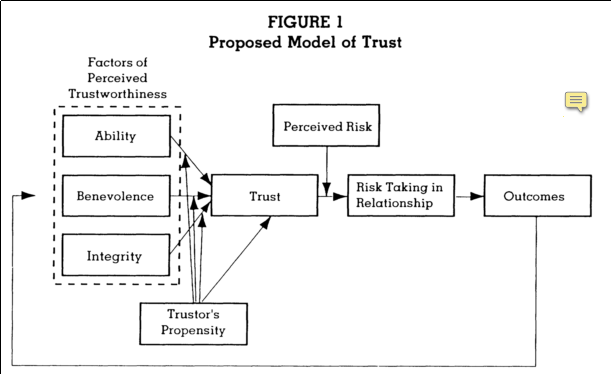
\includegraphics[width=\textwidth]{mayer1995-fig1}
  \caption[Model of Trust]{Model of Trust \cite{Mayer1995}}
  \label{fig:mayer_trust_model}
\end{figure}
Lee and See \cite{Lee2004} extended and synthesised Mayer et al's approach to personal and interpersonal trust towards a generalised concept of trust for human and autonomic/autonomous systems with the following alternative contextual definitions (including their approximate mappings to Mayer et al's approach
\begin{table}
  \caption[Factors of Trust for Autonomous Systems]{Factors of Trust for Autonomous Systems\cite{Lee2004}}
  \label{tab:autonomous_trust_factors}
  \begin{tabularx}{\textwidth}{p{2cm}X p{2cm}}\toprule
    Factor & Definition & Mayer Term\\ \midrule
    Performance & `The current and historical operation of the automation, including characteristics such as reliability, predictability, and ability & Ability\\
    Process & The degree to which the automation's algorithms are appropriate for the situation and able to achieve the operators goals.
    & Integrity\\
    Purpose & The degree to which the automation is being used within the realm of the designers intent & Benevolence \\
    \bottomrule
  \end{tabularx}
\end{table}


\subsection{Characteristics of Trust Relationships}

There are five commonly considered characteristics or attributes of Trust relationships in general, but not all relationships exhibit them and they are not assumed to be a complete specification of Trust:

\begin{itemize}
  \item \emph{Multi-Party} - One-to-one; one-to-many; many-to-one; many-to-many.
    Trust is not an absolute characteristic of a lone individual.
    Trust may include multi-agent abstractions (one-to-many), such as a preferential trust/distrust towards a group exhibiting a particular attribute, e.g.\ members of the armed forces / police services.
    Likewise, there can be trustor/trustee attributes that can generalise relationships between collectives (many-to-many), e.g.\ Jets and Sharks
  \item \emph{Transitive} - Trust assessments can be shared (i.e.\ recommendations), where this second order trust assessment incorporates both the observed trustworthiness of the trustee, as well as the trustworthiness of the intermediate trustor.
    In some models this is further extended to include out-of-network intermediate trustors that have some other defined authority, e.g.\ PKI Certificate Authority
  \item \emph{Evidential} - Trust must be based on some form of evidence-based observation or assessment, such as historical success rates of performing a certain action, or second-hand observations of trust from a third party.
  \item \emph{Directional Asymmetry} - The majority of relationships are bi-directional but are asymmetric, i.e.\ between two entities who ``trust'' each other, there are two independent trust relationships that may have very different ``values'' or extents.
  \item \emph{Contextual} - Trust can be variable and loosely coupled between contexts with respect to the action being assessed or the environment within which the trustee is operating, e.g.
    Doctors are trusted to perform medical procedures but that trust may not improve their success at correctly wiring an electrical plug.
    However there are plenty of counter-examples to this, as from \cite{Mayer1995}, two of the three listed factors of trust are ``Benevolence'' and ``Integrity'' and are unrelated to the ability of a trustee to perform a particular action, so it is reasonable to make an initial assumption that if a trustee is being benevolent in one activity or context, that that benevolence \emph{should} extend to other contexts.

\end{itemize}
\subsection{Topologies of Trust Networks}
\label{sec:trust_topologies}
Beyond the attributes or characteristics of an individual trust relationship, within any multi party sparsely connected network or community, topological context is useful in both establishing trust and in disseminating observations for collaborative assessment.

\missingfigure{Trust Topologies, Direct, Indirect, Recommender, etc.
We've done it a dozen times before, may as well make a new graphic}

\section{Trust in \gls{manet}s}
\subsection{Trust Perspectives in Autonomous Operation}
For the purposes of this work we define two perspectives on trust for autonomous systems: Design and Operational.
These are summarised in Table~\ref{tab:trust_perspectives}.
It is useful to further define and classify Operational Trust into two distinct but related sections defined in Table~\ref{tab:operational_trust_perspectives}.\todo{Work out how to reference across chapters in a multi doc}
\begin{table}
  \begin{tabularx}{\textwidth}{p{3cm}X}\toprule
    \emph{Design Trust} & When an autonomous system is under development a level of Trust is established in it through the manner in which it has been designed and tested.
    This is the same as conventional systems.\par
    Given that systems that have high-levels of autonomy are designed to behave adaptively to dynamic environments, it is challenging to fully predict such non-deterministic behaviours prior to operational deployment.
    For example, in a navigation system it is difficult to predict the dynamic environment it will need to adapt to.\par
    Trust needs to be developed that the design and test of such systems are sufficient to predict that operation will be, if not optimal, at least satisfactory.
    \\
    \emph{Operational Trust} & Trust at runtime or in-situ that both the individual nodes within a system are operating as expected and that the interfaces between the operator and the system are as expected.
    \par
    This latter aspect covers issues such as physical/wireless links and interpretation of data at each end of such a communication link.
    Operational Trust is functionally derived from, but distinct from Design Trust.\\
    \bottomrule
  \end{tabularx}
  \caption{Trust Perspectives with respect to autonomous systems}
  \label{tab:trust_perspectives}
\end{table}
\begin{table}
  \begin{tabularx}{\textwidth}{p{3cm}X}\toprule
    \emph{Hard Trust} or technical trust & The quantitative measurement and communication of the expectation of an actor performing a certain task, based on historic performance and through consensus building within a networked system.\par
    Can be thought of as a de-risking strategy to measure and monitor the ability of a system, or another actor within a system, to perform a task unsupervised.\\
    \emph{Soft Trust} or common trust & The qualitative assessment of the ability of an actor to perform a task or operation consistently and reliably based on social or experiential factors.\par
    This is the ‘human’ form of trust and is the main motivational driver for the human-factors trust discussion in *OTHER CHAPTER*.\par
    Can be rephrased as the level of confidence an operator has in an actor to perform a task unsupervised.\\
    \bottomrule
  \end{tabularx}
  \caption{Trust Perspectives within Operational Trust}
  \label{tab:operational_trust_perspectives}
\end{table}

It is already clear that these two definitions are extremely close in their construction, but represent fundamentally different approaches to trust, one coming from a sociological perspective of person-to-person and person-to-group relationships from day to day life, and the other coming from a statistical or formal appraisal of an activity by a system.
For the purposes of this work, we are concerned with the analytical establishment of hard trust within a topologically dynamic network of autonomous actors.

\subsection{Levels of Trust}
\todo{This section may be superfluous}
Trust relationships operate as part of a system architecture, and can quite often get confused.
Sun\cite{Sun2008} suggests that within these there are two overarching forms of trust:
\begin{itemize}
  \item Behavioural: That one entity voluntarily depends on another entity in a specific situation
  \item Intentional: That one entity would be willing to depend on another entity
\end{itemize}
These concepts closely mirror the previous definitions of ‘Hard’ and ‘Soft’ trust respectively, one (Behavioural) being an invested dependency given certain parameters being satisfied, mirroring Hard Trust, and the other (Intentional) being the ‘capacity for belief’ in another entity, analogous to Soft Trust.
It is suggested that these overarching forms are supported by and indeed are drawn from four major constructs within social and networked environments:
\begin{itemize}
  \item Trusting Belief: the subjective belief within a system that the other trusted components are willing and able to act in each-others’ best interests
  \item Dispositional Trust: a general expectation of trustworthiness over time 
  \item Situational Decision Trust: in-situ risk assessment where the benefits of trust outweigh the negative outcomes of trust
  \item System Trust: the assurance that formal impersonal or procedural structures are in place to ensure successful operation.
\end{itemize}
Sun argues that only System Trust and Behavioural Trust are relevant to trusted networking applications.
However, it is arguable that in any network where the operation of that network is not the only concern, or where that network has to interact with any operator, then all of these factors come into play.
Both System and Behavioural trust rely on what Sun calls a ‘Belief Formation Process’, or a trust assessment, while the other trust constructs deal with the interactions between trust and decision making against an internal assessment of network trustworthiness.

\subsection{Trust Model Design Considerations}
Trust is the level of confidence one agent has in another to perform a given action on request or in a certain context.
Trust in the autonomous or semi-autonomous realm is the ability of a system to establish and maintain confidence in itself or another systems' operations.
Managing this trust can be used to predict and reason on the future interactions between entities in a system, such as an autonomous mobile ad-hoc network (\gls{manet}).

The distributed and dynamic nature of \gls{manet}s mean that it is difficult to maintain a trusted third party (TTP) or evidence based trust system such as Certificate Authorities or using Public Key Infrastructures (PKI).\todo{possibly worthwhile doing more background on the operation of these}
Therefore, a distributed, collaborative system must be applied to these networks.
Such distributed trust management frameworks aim to detect, identify, and mitigate the impacts of malicious actors by distributing per-node assessments and opinions to collectively self-police behaviour.

As mobile ad-hoc networks (\gls{manet}s) grow beyond the terrestrial arena, their operation and the protocols designed around them must be reviewed to assess their suitability to different communications environments, ensuring their continued security, reliability, and performance.

Trust Management Frameworks (TMFs) provide information to assist the estimation of future states and actions of nodes within networks.
This information is used to optimize the performance of a network against malicious, selfish, or defective misbehaviour by one or more nodes.
Previous research has established the advantages of implementing TMFs in 802.11 based \gls{manet}s, particularly in terms of preventing selfish operation in collaborative systems \cite{Li2007}, and maintaining throughput in the presence of malicious actors \cite{Buchegger2002}
There are five topics that are important to address in any \gls{manet}s trust model \cite{Kamvar2003}:
\begin{itemize}
  \item The trust model should be without infrastructure.
    Because the network routing infrastructure is formed in an ad-hoc fashion, the trust management can not depend on, e.g., a trusted third party (TTP).
    There is no public key infrastructure (PKI), where some center nodes monitor the network, and publish illegal nodes periodically.
    In a \gls{manet}, there are no certification authorities (CA) or registration authorities (RA) with elevated privileges etc.
  \item The trust model should be anonymous because of the anonymity of mobile nodes in \gls{manet}s.
  \item The trust model should be robust.
    That is, it can be robust to all kinds of unfriendly attacks and the network itself should not be susceptible to attacks by unfriendly nodes.
    Moreover, in the presence of malicious nodes, they may attempt to subvert the model in order to get the unfairly good trust value.
  \item The trust model should have minimal control overhead in accordance with computation, storage, and complexity.
  \item The trust model should be self-organized.
    \gls{manet}s are characterized to have dynamic, random, rapidly changing and multi-hop topologies composed of variably bandwidth-constrained links
\end{itemize}
\section{Current Trust Management Frameworks}
Distributed trust management frameworks for \gls{manet}s aim to detect, identify, and mitigate the impacts of malicious actors by distributing per-node assessments and opinions to collectively self-police behaviour.
Various models and algorithms for describing trust and developing trust management in distributed systems, P2P communities or wireless networks have been considered.
Taking some examples;
\begin{itemize}
  \item \emph{Hermes Trust Establishment Framework} takes a Bayesian Beta function to model per-link Packet Loss Rate (PLR) over time, combining ``Trust'' and ``Confidence of Assessment'' into a single value \cite{Zouridaki2005}.
  \item \emph{The Objective Trust Management Framework} takes a Bayesian approach and introduces the idea of applying a Beta function to changes in the per-link Packet Loss Rate (PLR) over time, combining ``Trust'' and ``Confidence of Assessment'' into a single value \cite{Li2008}.
    \acrshort{otmf} however does not appropriately combat multi-node-collusion in the network \cite{Cho2011}.
  \item \emph{Trust-based Secure Routing \cite{Moe2008a}} demonstrated an extension to Dynamic Source Routing (DSR), incorporating a Hidden Markov Model of the wider ad-hoc network, reducing the efficacy of Byzantine attacks, particularly black-hole attacks but is limited by focusing on single metric observation (PLR)\cite{Cho2011}.
  \item \emph{CONFIDANT}; \cite{Buchegger2002} presented an approach using a probabilistic estimation of normal observations, similar to \acrshort{otmf}.
    They also introduced a greedy topology weighting scheme that internally weighted incoming trust assessments based on historical experience of the reporter.
  \item \emph{Fuzzy Trust-Based Filtering}; \cite{Luo2008} presented a method using Fuzzy Inference to cope with imperfect or malicious recommendation based on a probabilistic estimation of performance using conditional similarity to classify performance using overlapping Fuzzy Set Membership functions to collaboratively filter reputations across a network.
  \item \emph{Multi-parameter Trust Framework for \gls{manet}s (\acrshort{mtfm})} uses a number of communications metrics together for form a vector of trust, apply grey information theory to allow a system to detect and identify the tactics being used to undermine or subvert trust\cite{Guo11}
\end{itemize}
\subsection{Single Metric Trust Frameworks}
\todo{Expand background detail on more frameworks}
The Hermes trust establishment framework \cite{Zouridaki2005} uses Bayesian reasoning to generate a posterior distribution function of ``belief'', or trust, given a sequence of observations of that behaviour, $p(B|O)$\eqref{eq:otmf_pbo}.

\begin{equation}
  p(B|O)  = \frac{p(O|B) \times p(B)}{\rho}
  \label{eq:otmf_pbo}
\end{equation}
Where $p(B)$ is the prior probability density function for the expected normal behaviour, and $\rho$ is a normalising factor.
Due to it's flexibility and simplicity, Hermes assumes that $p(B)$ is a Beta function, and therefore the evaluation of this trust assessment is based around the expectation value of the distribution \eqref{eq:otmf_t}  where $\alpha$ and $\beta$ represent the number of successful and unsuccessful interactions respectively for a particular node $i$.

A secondary measurement of the confidence factor of the trust assessment $t$ is generated as \eqref{eq:otmf_c} and these measurements are combined to form a ``trustworthiness'' value $T$ \eqref{eq:otmf_trust}.

\begin{align}
  t_i &\to E\lbrack\text{beta}(p|\alpha,\beta)\rbrack = \frac{\alpha_i}{\alpha_i+\beta_i} \label{eq:otmf_t}\\[5pt]
  c_i &= 1 - \sqrt{\frac{12\alpha_i\beta_i}{(\alpha_i+\beta_i)^2(\alpha_i+\beta_i+1)}} \label{eq:otmf_c}\\[5pt]
  T_i &= 1 - \frac{\sqrt{\frac{(t_i-1)^2}{x^2} + \frac{(c_i-1)^2}{y^2}}}{\sqrt{\frac{1}{x^2}+\frac{1}{y^2}}} \label{eq:otmf_trust}
\end{align}
In \eqref{eq:otmf_trust}, $x$ and $y$ are constants, used weight the two-dimensional polar mapping of trust and confidence assessments ($t_i,c_i$), and from \cite{Zouridaki2005}, are taken as $x=\sqrt{2},y=\sqrt{9}$.

Upon this per-node assessment methodology, \acrshort{otmf} overlays an observation distribution protocol so as to make the measurements $\alpha_i$ and $\beta_i$ representative of the direct and 1-hop networks observations of the target node $i$, as well as expiring old observations from assessment and eliminating observations from ``untrustworthy'' nodes.

\todo{Want at least CONFIDANT and Fuzzy in here for contrast}
To date this work has been mostly limited to terrestrial, RF based networks.
There are also situations where the observed metrics will include significant noise and occur at irregular, sparse, intervals.
Conventional approaches such as probabilistic estimation do not produce trust values that reflect the underlying reality and context of the metrics available, as they require a-priori assumption that the trust value under exploration has an expected distribution, that distribution is mono-modal, and the input metrics are binary.
In scenarios with variable, sparse, noisy metrics, estimating the distribution is difficult to accomplish a-priori.

Hermes, \acrshort{otmf}, CONFIDANT, and Fuzzy Trust-Based Filtering can be generalised as single-value probabilistic estimation, based on a Bayesian idea of taking a binary input state and generating an idealised Beta Distribution (\ref{eq:beta}) of the future states of that input generated through an expectation value based on interactions (\ref{eq:beta_e}).
\begin{align}
  \label{eq:beta}
  \text{beta}(p|\alpha,\beta) = \frac{\Gamma(\alpha + \beta)}{\Gamma(\alpha)\Gamma(\beta)}p^{\alpha-1},\text{where } 0 \leq p \leq 1; \alpha,\beta > 0\\
  \label{eq:beta_e}
  E(p) = \frac{\alpha}{\alpha + \beta}
\end{align}
Where $\alpha$ and $\beta$ represent the number of successful and unsuccessful interactions respectively.

These single metric TMFs provide malicious actors with a significant advantage if their activity is undetectable by that one assessed metric, especially if the attacker is aware of the observed metric in advance.

The objective of operating a TMF is to increase the confidence in, and efficiency of, a system by reducing the amount of undetectable negative operations an attacker can perform.
In the case where the attacker can subvert the TMF, the metric under assessment by that TMF does not cover the threat mounted by the attacker.
In turn, this causes a super-linearly negative effect in the efficiency of the network as the TMF is assumed to have reduced the possible set of attacks when in fact it has only made it more advantageous to attack a different aspect of the networks operation.
An example of such a behaviour would be the case in a TMF focused on PLR where an attacker selectively delays packets going through it, reducing the over all throughput of one or more virtual network routes.
Such behaviour would not be detected by the TMF.

\subsection{Multi-Metric Trust Frameworks}\label{sec:multimetrictrust}
Given the potential incentives to a selfish attacker and potential threats to trust and fairness in sparse, noisy, and constrained environments, single metric trusts discussed above do not suitably cover the exposed threat surface.\todo{Probably best to just send a reference forward to the Marine Comms chapter}
A multi-metric approach may be more appropriate to capture and monitor the realities of harsh and sparse communications environments.

\acrshort{mtfm}\cite{Guo11} uses Grey Theory\cite{Zuo1995} to perform cohort based normalization of metrics at runtime, providing a ``grey relational grade'' of trust compared to other observed nodes in that interval for individual metrics, while maintaining the ability to reduce trust values down to a stable assessment range for decision support without requiring every environment entered into to be characterised.
This presents a stark difference between the Grey and Probabilistic approaches.
Grey assessments are relative in both fairly and unfairly operating networks.
All nodes will receive mid-range trust assessments if there are no malicious actors as there is nothing ``bad'' to compare against, and variations in assessment will be primarily driven by topological and environmental factors.
Guo et al.\cite{Guo11} demonstrated the ability of grey relational analysis (GRA) to normalise and combine disparate traits of a communications link such as instantaneous throughput, received signal strength, etc.\ into a grey relational coefficient (GRC), or a ``trust vector'' in this instance.

The grey relational vector is given as
%
\begin{align}
  \label{eq:grc}
  \theta_{k,j}^t = \frac{\min_k|a_{k,j}^t - g_j^t| + \rho \max_k|a_{k,j}^t-g_j^t|}{|a_{k,j}^t-g_j^t| + \rho \max_k|a_{k,j}^t-g_j^t|} \\
  \phi_{k,j}^t = \frac{\min_k|a_{k,j}^t - b_j^t| + \rho \max_k|a_{k,j}^t-b_j^t|}{|a_{k,j}^t-b_j^t| + \rho \max_k|a_{k,j}^t-b_j^t|} \notag 
\end{align}
%
where $a_{k,j}^t$ is the value of an observed metric $x_j$ for a given node $k$ at time $t$, $\rho$ is a distinguishing coefficient set to $0.5$, $g$ and $b$ are respectively the ``good'' and ``bad'' reference metric sequences from $\{a_{k,j}^t k=1,2\dots K\}$, i.e.\ $g_j=\max_k({a_{k,j}^t})$,  $b_j=\min_k({a_{k,j}^t})$ (where each metric is selected to be monotonically positive for trust assessment, e.g.\ higher throughput is presumed to be always better).

Weighting can be applied before generating a scalar value \eqref{eq:metric_weighting} allowing the detection and classification of misbehaviours.

%
\begin{equation}
  \label{eq:metric_weighting}
  [\theta_k^t, \phi_k^t] = \left[\sum_{j=0}^M h_j \theta_{k,j}^t,\sum_{j=0}^M h_j \phi_{k,j}^t \right]
\end{equation}
%
Where $H=[h_0\dots h_M]$ is a metric weighting vector such that $\sum h_j = 1$, and in unweighted case, $H=[\frac{1}{M},\frac{1}{M}\dots\frac{1}{M}]$.
$\theta$ and $\phi$ are then scaled to $[0,1]$ using the mapping $y = 1.5 x - 0.5$.
To minimise the uncertainties of belonging to either best ($g$) or worst ($b$) sequences in \eqref{eq:grc} the $[\theta,\phi]$ values are reduced into a scalar trust value by $T_k^t = ({1+{(\phi_k^t)^2}/{(\theta_k^t)^2}})^{-1}$ \cite{Hong2010}.
\acrshort{mtfm} combines this GRA with a topology-aware weighting scheme \eqref{eq:networkeffects} and a fuzzy whitenization model \eqref{eq:whitenization}.

There are three classes of topological trust relationship used; Direct, Recommendation, and Indirect, repeating those discussed in section~\ref{sec:trust_topologies}.\todo{This is currently half empty}
Where an observing node $n_i$ assesses the trust of another target node, $n_j$; the Direct relationship is $n_i$'s own observations $n_j$'s behaviour.
In the Recommendation case, a node $n_k$ which shares Direct relationships with both $n_i$ and $n_j$, gives its assessment of $n_j$ to $n_i$.
In the Indirect case, similar to the Recommendation case, the recommender $n_k$ does not have a direct link with the observer $n_i$ but $n_k$ has a Direct link with the target node, $n_j$.
These relationships give node sets, $N_R$ and $N_I$ containing the nodes that have recommendation or indirect, relationships to the observing node respectively.
%
\begin{align}
  \label{eq:networkeffects}
  T_{i,j}^{\acrshort{mtfm}}=&\frac{1}{2} \cdot \max_s\{f_s(T_{i,j})\} T_{i,j}\\ \notag
  +&\frac{1}{2} \frac{2|N_R| }{2|N_R| + |N_I|}\sum_{n \in N_R} \max_s\{f_s(T_{i,n})\} T_{i,n}\\ \notag
  +&\frac{1}{2} \frac{|N_I| }{2|N_R| + |N_I|}\sum_{n \in N_I} \max_s\{f_s(T_{i,n})\} T_{i,n} 
\end{align}
Where $T_{i,n}$ is the subjective trust assessment of $n_i$ by $n_n$, and $f_s = [ f_1,f_2, f_3]$ given as:
\begin{align}
  \label{eq:whitenization}
  f_1(x)&= -x+1\notag\\
  f_2(x)&= 
  \begin{cases}
    2x & \text{if }x\leq 0.5\\
    -2x+2 & \text{if }x>0.5
  \end{cases}\\
  f_3(x)&= x\notag
\end{align}
%
In the case of the terrestrial communications network used in \cite{Guo11}, the observed metric set $X = {x_1,\dots,x_M}$ representing the measurements taken by each node of its neighbours at least interval, is defined as $X=[$packet loss rate, signal strength, data rate, delay, throughput$]$.

Guo et al.\ demonstrated that when compared against \acrshort{otmf} and Hermes trust assessment, \acrshort{mtfm} provided increased variation in trust assessment over time, providing more information about the nodes' behaviours than packet delivery probability alone can.

\section{Grey System Theory and Grey Trust Assessment}
\todo{This section largely repeats from \acrshort{mtfm} discussion but the maths needs explored somewhere}
\subsection{Grey numbers, operators and terminology}
Grey numbers are used to represent values where their discrete value is unknown, where that number may take its possible value within an interval of potential values, generally written using the symbol $\oplus$.
Taking $a$ and $b$ as the lower and upper bounds of the grey interval respectively, such that $\oplus \in [a,b] | a < b$ 
The ``field'' of $\oplus$ is the value space $[a,b]$.
There are several classifications of grey numbers based on the relationships between these bounds.\todo{don't think classification is the right word here}
Black and White numbers are the extremes of this classification; such that $\dot\oplus \in [-\infty, +\infty]$ and $\mathring\oplus \in [x, x] | x \in \mathbb{R}$ or $\oplus(x)$
It is clear that white numbers such as $\mathring\oplus$ have a field of zero while black numbers have an infinite field.

Grey numbers may represent partial knowledge about a system or metric, and as such can represent half-open concepts, by only defining a single bound; for example $\underline\oplus = \oplus(\underline x ) \in [x, +\infty]$ and $\overline\oplus = \oplus(\overline x) \in [-\infty, x]$.

Primary operations within this number system are as follows;
\begin{subequations}
  \begin{align}
    \oplus_1 + \oplus_2      &\in [a_1+a_2,b_1+b_2] \label{eq:grey_add}\\
    -\oplus         &\in [-b,-a] \label{eq:grey_neg} \\
    \oplus_1 - \oplus_2      &= \oplus_1+(-\oplus) \label{eq:grey_sub}\\
    \oplus_1 \times \oplus_2 &\in \begin{aligned}[t]
      &[\min(a_1 a_2, a_1 b_2, b_1 a_2, b_2 a_2), \\
      & \max(a_1 a_2, a_1 b_2, b_1 a_2, b_2 a_2)]
    \end{aligned} \label{grey_mult}\\
    \oplus^{-1} &\in [b^{-1}, a^{-1}] \label{eq:grey_inv}\\
    \oplus_1 / \oplus_2 & = \oplus_1 \times \oplus_2^{-1} \label{grey_mult} \\
    \oplus \times k &\in [ka,kb] \label{eq:grey_times_scalar}\\
    \oplus^k &\in [a^k, b^k] \label{eq:grey_exp}
  \end{align}
\end{subequations}
where $k$ is a scalar quantity.

\subsection{Whitenisation and the Grey Core}
The characterisation of grey numbers is based on the encapsulation of information in a grey system in terms of the grey numbers core ($\hat\oplus$) and it's degree of greyness ($g^\circ$).
If the distribution of a grey number field is unknown and continuous, $\hat\oplus = \frac{a + b}{2}$.

Non-essential grey numbers are those that can be represented by a white number obtained either through experience or particular method.
\cite{Liu2011}
This white hissed value is represented by $\tilde\oplus$ or $\oplus(x)$ to represent grey numbers with $x$ as their whitenisation.
In some cases depending on the context of application, particular gray numbers may temporarily have no reasonable whitenisation value (for instance, a black number).
Such numbers are said to be Essential grey numbers.

\subsection{Grey Sequence Buffers and Generators}
\todo{eqs of sequence buffers and partial derivs}
Given a fully populated value space, sequence buffer operations are used to provide abstractions over the dataspace.
These abstractions can be \emph{weakening} or \emph{strengthening}.
In the weakening case, these operations perform a level of smoothing on the volatility of a given input space, and strengthening buffers serve to highlight and 
A powerful tool in grey system theory is the use of grey incidence factors, comparing the ``likeness'' of one value against a cohort of values.
This usefulness applies particularly well in the case of multi-agent trust networks, where the aim is to detect and identify malicious or maladaptive behaviour, rather than an absolute assessment of ``trustworthiness''.

\subsection{Grey Trust}
Grey Theory performs cohort based normalization of metrics at runtime.
This creates a more stable contextual assessment of trust, providing a ``grade'' of trust compared to other observed entities in that interval, while maintaining the ability to reduce trust values to a stable assessment range for decision support without requiring every environment entered into to be characterised.
Grey assessments are relative in both fairly and unfairly operating cohorts.
Entities will receive mid-range trust assessments if there are no malicious actors as there is no-one else ``bad'' to compare against.

Guo\cite{Guo11} demonstrated the ability of Grey Relational Analysis (GRA)\cite{Zuo1995} to normalise and combine disparate traits of a communications link such as instantaneous throughput, received signal strength, etc.\ into a Grey Relational Coefficient, or a ``trust vector''.

In \cite{Guo11}, the observed metric set $X = {x_1,\dots,x_M}$ representing the measurements taken by each node of its neighbours at least interval, is defined as $X=[$packet loss rate, signal strength, data rate, delay, throughput$]$.
The trust vector is given as
%
\begin{align}
  \label{eq:grc}
  \theta_{k,j}^t = \frac{\min_k|a_{k,j}^t - g_j^t| + \rho \max_k|a_{k,j}^t-g_j^t|}{|a_{k,j}^t-g_j^t| + \rho \max_k|a_{k,j}^t-g_j^t|} \\
  \phi_{k,j}^t = \frac{\min_k|a_{k,j}^t - b_j^t| + \rho \max_k|a_{k,j}^t-b_j^t|}{|a_{k,j}^t-b_j^t| + \rho \max_k|a_{k,j}^t-b_j^t|} \notag 
\end{align}
%
where $a_{k,j}^t$ is the value of a observed metric $x_j$ for a given node $k$ at time $t$, $\rho$ is a distinguishing coefficient set to $0.5$, $g$ and $b$ are respectively the '``good'' and ``bad'' reference metric sequences from $\{a_{k,j}^t k=1,2\dots K\}$, e.g.\ $g_j=\max_k({a_{k,j}^t})$,  $b_j=\min_k({a_{k,j}^t})$ (where each metric is selected to be monotonically positive for trust assessment, e.g.\ higher throughput is always better).

Weighting can be applied before generating a scalar value which allows the identification and classification of untrustworthy behaviours.

%
\begin{equation}
  \label{eq:metric_weighting}
  [\theta_k^t, \phi_k^t] = \left[\sum_{j=0}^M h_j \theta_{k,j}^t,\sum_{j=0}^M h_j \phi_{k,j}^t \right]
\end{equation}
Where $H=[h_0\dots h_M]$ is a metric weighting vector such that $\sum h_j = 1$, and in the basic case, $H=[\frac{1}{M},\frac{1}{M}\dots\frac{1}{M}]$ to treat all metrics evenly.
$\theta$ and $\phi$ are then scaled to $[0,1]$ using the mapping $y = 1.5 x - 0.5$.
The $[\theta,\phi]$ values are reduced into a scalar trust value by $T_k^t = ({1+{(\phi_k^t)^2}/{(\theta_k^t)^2}})^{-1}$.
This trust value minimises the uncertainties of belonging to either best ($g$) or worst ($b$) sequences in \eqref{eq:grc}.

\acrshort{mtfm} combines this GRA with a topology-aware weighting scheme\eqref{eq:networkeffects} and a fuzzy whitenization model\eqref{eq:whitenization}.
There are three classes of topological trust relationship used; Direct, Recommendation, and Indirect.
Where an observing node, $n_i$, assesses the trust of another, target, node, $n_j$; the Direct relationship is $n_i$'s own observations $n_j$'s behaviour.
In the Recommendation case, a node $n_k$, which shares Direct relationships with both $n_i$ and $n_j$, gives its assessment of $n_j$ to $n_i$.
The Indirect case, similar to the Recommendation case, the recommender $n_k$, does not have a direct link with the observer $n_i$ but $n_k$ has a Direct link with the target node, $n_j$.
These relationships give us node sets, $N_R$ and $N_I$ containing the nodes that have recommendation or indirect, relationships to the observing node respectively.
%
\begin{align}
  \label{eq:networkeffects}
  T_{i,j}^{\acrshort{mtfm}}=\frac{1}{2} \cdot \max_s\{f_s(T_{i,j})\} T_{i,j}+&\frac{1}{2} \frac{2|N_R| }{2|N_R| + |N_I|}\sum_{n \in N_R} \max_s\{f_s(T_{i,n})\} T_{i,n}\\ \notag
  +&\frac{1}{2} \frac{|N_I| }{2|N_R| + |N_I|}\sum_{n \in N_I} \max_s\{f_s(T_{i,n})\} T_{i,n} 
\end{align}
Where $T_{i,n}$ is the subjective trust assessment of $n_i$ by $n_n$, and $f_s = [ f_1,f_2, f_3]$ given as:
\begin{align}
  \label{eq:whitenization}
  f_1(x)&= -x+1\notag\\
  f_2(x)&= 
  \begin{cases}
    2x & \text{if }x\leq 0.5\\
    -2x+2 & \text{if }x>0.5
  \end{cases}\\
  f_3(x)&= x\notag
\end{align}
Grey System Theory, by it's own authors admission, hasn't taken root in it's originally intended area of system modelling \cite{Liu2011}.
However, given it's tentative application to \gls{manet} trust, taking a Grey approach on a per metric benefit has qualitative benefits that require investigation; the algebraic approach to uncertainty and the application of ``essential and non essential greyness'', whiteisation, and particularly grey buffer sequencing allow for the opportunity to generate continuous trust assessments from multiple domains asynchronously.

\section{Conclusion}
As mobile ad-hoc networks (\gls{manet}s) grow beyond the terrestrial arena, their operation and the protocols designed around them must be reviewed to assess their suitability to different communications environments to ensure their continued security, reliability, and performance.
With demand for smaller, more decentralised \gls{manet} systems in a range of domains and applications, as well as a drive towards lower per-unit cost in all areas, TMFs are going to be increasingly applied to resource constrained applications, as the benefits and efficiencies they present are significant.
Beyond the constraints of the communications environment, knock on pressures in battery capacity, on-board processing, and locomotion simultaneously present opportunities and incentives for malicious or selfish actors to appear to cooperate while not reciprocating, in order to conserve power for instance.
These multiple aspects of potential incentives, trust, and fairness do not directly fall under the scope of single metric trusts discussed above, and this context indicates that a multi-metric approach may be more appropriate.
These increasingly decentralised applications present unique threats against trust management \cite{Caiti2011}.

One area of application is the underwater marine environment, where extreme challenges to communications present themselves (propagation delays, frequency dependent attenuation, fast and slow fading, refractive multipath distortion, etc.).
In addition to the communications challenges, other considerations such as command and control isolation, as well as power and locomotive limitations, drive towards the use of teams of smaller and cheaper \acrfull{auv} platforms.
In underwater environments, communications is both sparse and noisy.
Therefore the observations about the communications processes that are used to generate the trust metrics, occur much less frequently, with much greater error (noise) and delay than is experienced in terrestrial RF \gls{manet}S.

As such, the use of trust methods developed in the terrestrial \gls{manet} space should be reappraised for application within the underwater context \cite{Pavan2015}.

In the next chapter, the marine communications environment will be studied, as will the current state of the art in the use of autonomy in specifically defence related maritime applications.
%%%%%%%%%%%%%%%%%%%%%%%%%%%%%%%%%%%%%%%%%%%%%%%%%%%%%%%%%%%%%%%%%%%%%%%%%%%%%%%
\ifx\ifthesis\undefined
%% ----------------------------------------------------------------
\label{Bibliography}
% \bibliographystyle{amsplain}
%\bibliographystyle{unsrtnat}  % Use the "unsrtnat" BibTeX style for formatting the Bibliography
\bibliographystyle{alpha}
\bibliography{../Thesis}  % The references (bibliography) information are stored in the file named "Thesis.bib"

\end{document}  % The End
%% ----------------------------------------------------------------
\else
\fi
 % Background on Trust and its Applications to MANETs

% !TeX spellcheck = en_GB
\def\ChapterTitle{Maritime Communications and Operations}

\chapter{\ChapterTitle}
\label{Chapter\thechapter}
\lhead{Chapter \thechapter.
\emph{\nameref{Chapter\thechapter}}} % Write in your own chapter title to set the page header

\section{Maritime Communications Environment}\label{sec:marine_comms}

The key challenges of underwater acoustic communications are centred around the impact of slow and differential propagation of energy (RF, Optical, Acoustic) through water, and it's interfaces with the seabed / air.
The resultant challenges include; long delays due to propagation, significant inter-symbol interference and Doppler spreading, fast and slow fading due to environmental effects (aquatic flora/fauna; surface weather), carrier-frequency dependent signal attenuation, multipath caused by the medium interfaces at the surface and seabed, variations in propagation speed due to depth dependant effects (salinity, temperature, pressure, gaseous concentrations and bubbling), and subsequent refractive spreading and lensing due to that same propagation variation\cite{Partan2006}.

\subsection{Mechanics of Acoustic Transmission}

Unlike in RF energy transfer (where photons move through space to transmit energy from one place to another), acoustic wages are the result of mechanical perturbation of a medium where localised compressions and extensions pass energy across a medium through that mediums elastic properties.
These ``compression waves'' propagate away from its source, and the rate of this propagation is the sound speed, velocity or $c$, measured in $ms^{-1}$.
This is not to be confused with the fluid velocity corresponding to the instantaneous motion of particles in the medium.

Hydrophones, like their more common microphone equivalent in air, are fundamentally pressure sensors.
Acoustic pressure is usually measured in \emph{Pascals} ($Pa/\mu Pa$). 
In the underwater environment, the dynamic range (difference between instantaneous high and low pressure values) may be extremely high, often more than 10 orders of magnitude higher. 
As such, logarithmic notation is justified.

Useful acoustic signals are generally maintained vibrations rather than instantaneous pulses.
They are characterised by their frequency $f$ expressed in Hertz ($Hz$) or by their Period ($T$) in seconds.
In commonly used underwater acoustics, used frequencies range from $\approx 10Hz-100kHz$ depending on application.\cite{Stojanovic2007}.

As with all waves, the relationship between frequency, period and the wavelength is given as in \eqref{eq:wavelength}. 
As such the generally used upper and lower bounds of wavelength in most applications is from $1.5 m @ 10Hz$ to $0.015m @ 100kHz$.
%
\begin{equation}
  \lambda = cT = \frac{c}{f}
  \label{eq:wavelength}
\end{equation}
%

This wide range of frequencies and wavelengths allow for a diverse set of constraining factors; (Paraphrased from \citet{lurton2010}).

\begin{itemize}
  \item \emph{Attenuation} in water; limiting the maximum usable range, which increases very rapidly with frequency
  \item \emph{Dimensions} of sound source; which increase at lower $f$ for a given transmission power
  \item \emph{Spatial Selectivity} of sources and receivers as $f$ increases, due to similarly increasing directivity of energy propagation.
  \item \emph{Acoustic Response} of target surfaces (analogous to receiver gain in RF networks.
\end{itemize}

\subsection{Velocity and density}

Air has a baseline density of approximately $1.3 kg m^{-3}$, and the speed of sound is typically static around $340 ms^{-1}$.
In sea water, acoustic wave velocity is close to $c=1500ms^{-1}$ (generally between $1450ms^{-1}$ and $1550ms^{-1}$ depending on temperature, pressure, salinity etc.).
Similarly variable is sea water density, which is nominally $\rho = 1030kg m^{-3}$.

While the sea/air surface is (ideally) a simple refractive interface, the interface between open seawater and marine sediment is graduated, with density ranges between $1200 - 2000 kg m^{-3}$. 
This results in refractive and reflective velocities in the sediment interface ranging from $1500-2000 ms^{-1}$\cite{lurton2010}.

For comparison, the speed of light in air/water is $2.99 \times 10^8 ms^{-1}$ and $2.249 \times 10^{8} ms^{-1}$ respectively. 
\todo{this might be better as a table}

\citet{Mackenzie1981} proposed a more accurate model of acoustic velocity incorporating archival data from 15 worldwide sites that takes Temperature, Salinity and Depth into consideration.

\begin{align}
  c = & 1448.96 + 4.591 T - 5.304 \times 10^{-2} T^2 + 2.374 \times 10^{-4}T^{3}\notag\\
  & +1.340 (S-35) + 1.630\times 10^{-2}D+1.675\times 10^{-7}D^2\\
  & -1.025 \times 10^{-2}T(S-25) - 7.139\times 10^{-13}TD^3\notag
  \label{equ:mackenzie}
\end{align}

Where $T$ is the temperature in Celsius, $S$ the salinity in parts per thousand, and $D$ is the depth below the surface in meters.

\todo{Need to discuss Speed of Sound Profiles}

\subsection{Intensity and Power} 

The energy of an acoustic wave is encapsulated into its kinetic and potential parts; where its kinetic energy corresponds to the active motion energy of the particles in the medium, and the potential energy corresponding to the elastic potential of the medium in displacement/compression.

The acoustic intensity ($I$) is the energy flux mean value per unit of surface and time \eqref{eq:acoustic_intensity} in Watts/$m^2$ where $p_0$ is the plane wave amplitude (pressure) and $P_{rms} = p_0/\sqrt{2}$

\begin{equation}
  I = \frac{p_0^2}{2\rho c} = \frac{p_{rms}^2}{\rho c}
  \label{eq:acoustic_intensity}
\end{equation}

\subsection{Attenuation}

The attenuation that occurs in an underwater acoustic channel over a distance $d$ for a signal about frequency $f$ in linear \eqref{eq:acoattenuation} and $dB$ forms \eqref{eq:acoattenuationdb} is given as;

\begin{equation}
  \label{eq:acoattenuation}
  A_{\text{aco}}(d,f) = A_0d^ka(f)^d
\end{equation}
\begin{equation}
  \label{eq:acoattenuationdb}
  10 \log A_{\text{aco}}(d,f)/A_0 = k \cdot 10 \log d + d \cdot 10 \log a(f)
\end{equation}

where $A_0$ is a unit-normalising constant, $k$ is a geometric spreading factor (commonly taken as 1.5 for practical use, but may be 2 for perfect spherical propagation or 1 for perfect plane-wave propagation)), and $a(f)$ is the absorption coefficient, that may be modelled in a variety of ways.

Thorp's formula (\autoref{eq:thorp}) is very simple, only depending on $f$, and is designed to be most accurate about a temperature of 4$^{\circ}$C at a depth of $\approx 1Km$.
%
\begin{figure}
  \begin{equation}
    10 \log a(f) = 0.11 \cdot \frac{f^2}{1+f^2} + 44\cdot\frac{f^2}{4100+f^2}+ 2.75\times10^{-4} f^2 + 0.003
    \label{eq:thorp}
  \end{equation}
  \caption[Thorp's formula]{Thorp's Absorption Model\cite{Stojanovic2007}}
    \label{fig:thorp}
\end{figure}
%
The Ainslie \& McColm model is more complex, and incorporates the acidity of the water ($H^+$) as well as temperature ($T$), salinity ($S$ in parts per trillion) but not depth (\autoref{fig:ainslie}).
%
\begin{figure}
  \begin{align}
    10 \log a(f) =& 0.106 \frac{t_1 f^2}{t_1^2 + f^2} e^{\frac{H^+-8}{0.56}}\\\notag
      & + 0.52 \left(1+\frac{T}{43}\right)\left(\frac{S}{35}\right)\frac{t_2f^2}{t_2^2+f^2} e^{\frac{-D}{6}}\\\notag
      & + 4.9 \times 10^{-4} f^2e^{-\left(\frac{T}{27}+\frac{D}{17}\right)}\\\notag
      \text{Where}&\\\notag
      t_1 =& 0.78 \sqrt{\frac{S}{35}e^{\frac{T}{26}}}\\\notag
      t_2 =& 42 e^{\frac{T}{17}}\notag
      \label{eq:ainslie}
  \end{align}
  \caption{Ainslie \& McColm Absorption Model}
  \label{fig:ainslie}
\end{figure}
%
\begin{figure}
  \begin{align}
    10 \log a(f)=& A_1P_1\frac{t_1f^2}{t_1^2+f^2} + A_2P_2\frac{t_2f^2}{t_2^2+f^2} + A_3P_3f^2\\\notag
    \text{Where }&\\\notag
    A_1=&1.03\times 10^{-8} + 2.36\times 10^{-10} \cdot T -5.22 \times 10^{-12}\cdot T^2\\\notag
    A_2=&5.62\times 10^{-8} + 7.52\times 10^{-10} \cdot T\\\notag
    A_3=&\left(55.9 - 2.39\cdot T + 4.77\times 10^{-2}\cdot T^2 - 3.48 \times 10^{-4}\cdot T^3\right) \times 10 ^{-15}\\\notag
    t_1=&1.32\times 10^3\left(T+273.1\right)e^{\frac{-1700}{T+273.1}}\\\notag
    t_2=&1.55\times 10^7\left(T+273.1\right)e^{\frac{-3052}{T+273.1}}\\\notag
    P_1=&1\\\notag
    P_2=&\-10.3\times 10^{-4}\cdot P + 3.7\times 10^{-7}\cdot P^2\\\notag
    P_3=&\-3.84\times 10^{-4}\cdot P + 7.57\times 10^{-8}\cdot P^2\notag
    \label{eq:fisher}
  \end{align}
  \caption{Fisher-Simmons Absorption Model}
  \label{fig:fisher}
\end{figure}
%
The Fisher-Simmons model (\autoref{fig:fisher}) is significantly more complex, taking into account the effects of boric acid concentrations and dissolved magnesium sulphate. While there are several limitations on this model in terms of its being fixed at a salinity of 35 ppt and a pH of 8, as this model incorporates depth, temperature, distance and frequency, it is very attractive for research directed at high variability environments.\todo{Possibly need to switch this with the Francois Garrison model which, depending on your source, is the refined version (or vise versa}



Regardless of the variations of particular attenuation models, comparing $A_{aco}(d,f)$ with the RF Free-Space Path Loss model $(A_{\text{RF}}(d,f) \approx \left( \frac{4\pi d f}{c} \right)^2)$, the impact of range on signal power is exponential underwater, rather than quadratic in terrestrial RF ($A_{\text{aco}} \propto f^{2d}$ vs $A_{\text{RF}} \propto (df)^2$). 
While both frequency dependant factors are quadratic, approximating the factors in \eqref{eq:thorp}, $f\propto A_{\text{aco}}$ is at least 4 orders of magnitude higher than $f\propto A_{\text{RF}}$
\begin{equation}
  \label{eq:fspl}
  A_{\text{RF}}(d,f) \approx \left( \frac{4\pi d f}{c} \right)^2
  \text{where }c\approx 3\times10^8ms^{-1}
\end{equation}Ó


 \subsection{Ambient Noise Model}

 Ambient ocean noise can be assumed to be Gaussian with a continuous power spectral density in dB re $\mu$Pa per Hz, driven by four major factors, shown in \autoref{tab:ocean_noise_factors} \cite{coates1989}.\todo{check what $s$ and $w$ are in this}

\begin{table}\centering
  \caption{Contributing factors to Ocean Ambient Acoustic Noise}
  \label{tab:ocean_noise_factors}
  \begin{tabularx}{\textwidth}{p{3.5cm} X}\toprule
    Source & Approximation \\ \midrule
    Turbulence & $10 \log N_t(f)=17-30\log f$\\
    Shipping & $10 \log N_s(f) = 40+20(s-0.5)+26\log f-60\log(f+0.03)$\\
    Wind Driven Waves & $10\log N_w(f) = 50+7.5w^{\frac{1}{2}}+20\log f - 40\log(f+0.4)$\\ 
    Thermal Noise & $10\log N_{th}(f) = \-15 + 20 log f$\\\bottomrule
  \end{tabularx}
\end{table}

\subsection{Multipath effects}

Refractive lensing and the multi-path nature of the medium result in line of sight propagation being extremely unreliable for estimating distances to targets.
The first arriving acoustic signal has as the very least curved in the medium, and commonly has reflected off the surface/seabed before arriving at a receiver, creating secondary paths that are sometimes many times longer than the first arrival path, generating symbol spreading over orders of seconds depending on the ranges and depths involved.
Thus, the multi-path channel transfer function can be described by 

\begin{align}
  \label{eq:acomultipath}
  H(d,f) =\sum_{p=0}^{P-1} h(p) = \sum_{p=0}^{P-1} \Gamma_p / \sqrt{A(d_p,f)}e^{-j 2 \pi f \tau_p} \\
  \text{where } \tau_p = d_p/c, c \approx 1500 ms^{-1} \notag
\end{align}

where $d=d_0$ is the minimal path length between the transmitter and receiver, $d_p,p=\{1,\dots P-1\}$ are the secondary path lengths, $\Gamma_p$ models additional losses incurred on each path such as reflection losses at the surface interface, and $\tau_p = d_p/c$ is the delay time.

\begin{figure}
  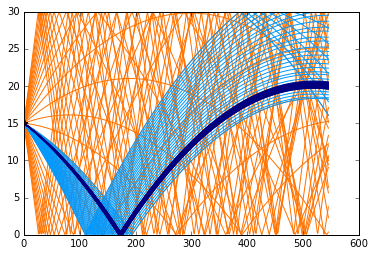
\includegraphics{ghia_sound_prop_curve}
  \caption{Non-Linear Marine Propagation in an isothermal profile}
  \todo[inline]{Vectorise and Label}
  \label{fig:ghia_sound_prop_curve}
\end{figure}



\subsection{Modelling and Simulation of the Acoustic Medium / Channel}

Several toolkits exist in a variety of states that perform communications agent simulation, most notably the NS-2 / 3 family of frameworks and their addons.
Some of these frameworks, such as SUNSET \cite{Petrioli2012a} and AquaTools \cite{Sehgal2010}.

Beyond the NS family, there are many other communications and simulation modelling systems such as OpNet++\cite{Chang1999} and MATLAB toolkits such as the AcTUP interface to the Ocean Acoustics Library.


\todo{expand this, justify AUVNetSim, reactive mobility, python compatibility, SimPy Etc.}


\subsection{Routing and Network Design for \glspl{uan}}

Forward Error Correction coding is used on such channels to minimise packet losses.

\todo{Summary of Akyildiz02/05}

\section{Marine Operations}\label{sec:marine_ops}

\subsection{Typical \gls{auv} mission profiles}

\todo{Typical AUV missions, payloads, and available equipment}

\subsection{Potential Future Applications}
\todo{Future Applications of AUVs}

\subsection{Need for Trust in Maritime Networks}

As \acrfull{auv} platforms become more capable and economical, they are being used in many applications requiring trust.
These applications are using the collective behaviour of teams or fleets of these \glspl{auv} to accomplish tasks \cite{Caiti2011}.
With this use being increasingly isolated from stable communications networks, the establishment of trust between nodes is essential for the reliability and stability of such teams.
As such, the use of trust methods developed in the terrestrial \gls{manet} space must be re-appraised for application within the challenging underwater communications channel.



%%%%%%%%%%%%%%%%%%%%%%%%%%%%%%%%%%%%%%%%%%%%%%%%%%%%%%%%%%%%%%%%%%%%%%%%%%%%%%%
 % Background on Maritime Uses of Autonomous Systems and the Maritime Communications Environment

% !TeX spellcheck = en_GB
\def\ChapterTitle{Assessment of TMF Performance in Marine Environments}

\ifx\ifthesis\undefined
\documentclass[a4paper, 11pt]{article}

% % Special Includes stolen from Thesis.cls
\usepackage{booktabs}
\usepackage{hyperref}
\usepackage{graphicx}
\usepackage{epstopdf}
\usepackage{subcaption}
\usepackage{rotating}
\usepackage{listings}
\usepackage{lstpatch}
\renewcommand{\arraystretch}{1.3}

% % % % % % % % % % % % % % % %

% PACKAGES
\usepackage[square, numbers, comma, sort&compress]{natbib}  % Use the "Natbib" style for the references in the Bibliography
\usepackage{verbatim,listings}  % Needed for the "comment" environment to make LaTeX comments
\usepackage{array}  % Needed for the "comment" environment to make LaTeX comments
\usepackage{vector}  % Allows "\bvec{}" and "\buvec{}" for "blackboard" style bold vectors in maths
\usepackage{amsmath,amsfonts,amsthm,color,psfrag,epsf, tabularx, multirow, longtable}
\usepackage{snapshot, todonotes}
% \usepackage{pstricks}
\usepackage{enumerate}
%\usepackage[lined,algonl,boxed]{algorithm2e}
\usepackage[ruled,linesnumbered,vlined]{algorithm2e}
\usepackage{float}
\usepackage{epigraph} % epigraph
\usepackage{tikz}
\usetikzlibrary{shapes.geometric, arrows}

\usepackage{setspace}
\doublespacing
% or:
%\onehalfspacing

% SETUP
\hypersetup{urlcolor=blue, colorlinks=false}  % Colours hyperlinks in blue, but this can be distracting if there are many links. 
\DeclareGraphicsExtensions{.pdf,.jpeg,.png}
\graphicspath{{../Figures/}{../../../Dropbox/Thesis_Figures/}}  % Location of the graphics files (set up for graphics to be in PDF format)

% NOTE THERES A FUCKUP IN TEX4HT http://tug.org/pipermail/tex4ht/2014q2/000944.html
% NEED TO MANUALLY CHANGE \def\pgfsys@svg@newline{{?nl}}
\ifdefined\HCode
\usepackage[compatibility=false]{caption}
\def\pgfsysdriver{pgfsys-tex4ht.def}
\else
\usepackage[]{caption}
\fi

% \SpecialCoor
\def\subsum{\mathit{\Sigma}}

%opening
\title{\ChapterTitle}
\author{Andrew Bolster}

\begin{document}

\maketitle

\else
\chapter{\ChapterTitle}
\label{Chapter\thechapter}
\lhead{Chapter \thechapter. \emph{\nameref{Chapter\thechapter}}} % Write in your own chapter title to set the page header
\fi



\section{Comparison of Terrestrial and Marine Communication Trust Assessments}

In this chapter, we demonstrate the need for multi-metric trust assessment in Underwater Autonomous Networks (UAN).
Many UANs use MANET architectures, however the marine environment presents new challenges for trust management frameworks that have been developed for use in conventional (i.e. Terrestrial RF) MANETs.
We investigate the operation of a selection of traditional MANET TMFs in this environment.
We characterise these challenges and present results that demonstrate a multi-metric approach to Trust greatly enhances the effectiveness of TMFs in these environments.

\subsection{Trust in Marine Networks}\label{sec:trust_in_marine}

With demand for smaller, more decentralised marine survey and monitoring systems, and a drive towards lower per-unit cost, TMFs are going to be increasingly applied to the marine space, as the benefits they present are significant.
Beyond the constraints of the communications environment, knock on pressures are applying in battery capacity, on-board processing, and locomotion.
These pressures simultaneously present opportunities and incentives for malicious or selfish actors to appear to cooperate while not reciprocating, in order to conserve power for instance.
These multiple aspects of potential incentives, trust, and fairness do not directly fall under the scope of single metric trusts discussed above, and this context indicates that a multi-metric approach may be more appropriate.

As mobile ad-hoc networks (MANETs) grow beyond the terrestrial arena, their operation and the protocols designed around them must be reviewed to assess their suitability to different communications environments to ensure their continued security, reliability, and performance.

One area of application is the underwater marine environment, where extreme challenges to communications present themselves (propagation delays, frequency dependent attenuation, fast and slow fading, refractive multi-path distortion, etc.).
In addition to the communications challenges, other considerations such as command and control isolation, as well as power and locomotive limitations, drive towards the use of teams of smaller and cheaper autonomous underwater vehicles (AUVs). 
These increasingly decentralised applications present unique threats against trust management \cite{Caiti2011}.
In underwater environments, communications is both sparse and noisy.
Therefore the observations about the communications processes that are used to generate the trust metrics, occur much less frequently, with much greater error (noise) and delay than is experienced in terrestrial RF MANETS.
As such, the use of trust methods developed in the terrestrial MANET space must be re-appraised for application within the underwater context \cite{Pavan2015}.

Trust Management Frameworks (TMFs) provide information to assist the estimation of future states and actions of nodes within networks.
This information is used to optimize the performance of a network against malicious, selfish, or defective misbehaviour by one or more nodes.
Previous research has established the advantages of implementing TMFs in 802.11 based MANETs, particularly in terms of preventing selfish operation in collaborative systems \cite{Li2007}, and maintaining throughput in the presence of malicious actors \cite{Buchegger2002}

Most current TMFs use a single type of observed action to derive trust values, typically successfully delivered or forwarded packets. 
These observations then inform future decisions of individual nodes, for example, route selection \cite{Li2008}.

Recent work has demonstrated the use of a number of metrics to form a ``vector'' of trust.
The Multi-parameter Trust Framework for MANETs (MTFM) \cite{Guo11}, uses a range of communications metrics beyond packet delivery/loss rate (PLR) to assess trust.
This vectorized trust also allows a system to detect and identify the tactics being used to undermine or subvert trust.
To date this work has been limited to terrestrial, RF based networks. 

\subsection{Establishing Scale Factors in Communications Rate}

In this section we characterise the simulated communications environment, establishing an optimal packet emission rate for comparison against \cite{Guo11}.

In order to establish the point at which the network becomes saturated due, a range of packet emission rates were explored between 0.01 packets per second (pps), equivalent to 96 bps, up to 0.07 pps (672 bps)

From Figs.~\ref{fig:throughput_performance_static} and ~\ref{fig:prod_breakdown_static}, it is clear that the threshold curve, expressed as the \emph{Successfully Received Packets} line, exhibits a saturation point between 0.025 and 0.03 pps.
Particularly in Fig.~\ref{fig:prod_breakdown_static}, the precipitous drop in packet delivery probability beyond 0.025 pps, indicating that this is a strong candidate value for an upper-limit to the safe operating zone in terms of packet emission in the small static case.

\begin{figure}[H]
	\centering
	%\missingfigure{throughput_performance_static}
	\caption{Varying packet emission rate demonstrates maximal throughput at 0.025 packets per second, equivalent to $\approx$240 bps}
	\label{fig:3d}
\end{figure}


\begin{figure}[H]
	\centering
	%\missingfigure{prod_breakdown_static}
	\caption{Varying packet emission rate demonstrates a saturation point at 0.025 packets per second}
	\label{fig:prod_breakdown_static}
\end{figure}



\subsection{Establishing Scale Factors in Physical Distribution}

In this section we characterise the effect of node-separation scaling on communications operation for comparison against \cite{Guo11}. This is particularly important considering the significant scale factor differences between not only the speed of propagation in the medium, but simply the range of operation. 
From Table \ref{tab:sysconstraints}, the operating transmission range of acoustic is $\approx 6$ times further than 802.11, indicating that a suitable operating environment will have an area $\approx \sqrt{6}$ times the area of the 802.11 case. Therefore, a reasonable experimental range would have an upper bound of performance around this scaling factor, where nodes are approximately 400$m$ apart. 

A reasonable range around this is to scale from 100$m$ apart on average to 800$m$.

Varying average node separation shows that while direct throughput isn't significantly affected until, collision rates are Fig.~\ref{fig:throughput_performance_range}.
This collision rate is well within the tolerances of the MAC layer, as shown in Fig.~\ref{fig:prod_breakdown_range}, where even with a rising collision rate, packets are being reliably received.

\begin{figure}[H]
	\centering
	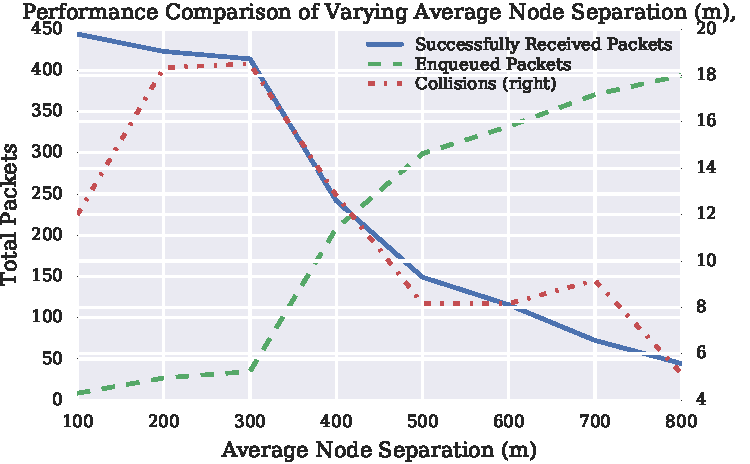
\includegraphics[width=0.6\textwidth]{throughput_performance_range.pdf}
	\caption{Comparison of Medium Acquisition Collisions, Throughput, and Enqueued packets against varying application packet emission rates.}
	\label{fig:throughput_performance_range}
\end{figure}

\begin{figure}[H]
	\centering
	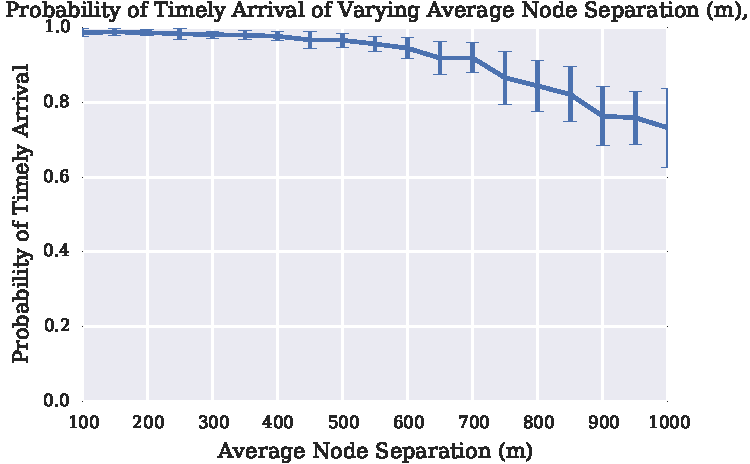
\includegraphics[width=0.6\textwidth]{prod_breakdown_range.pdf}
	\caption{Probability of Timely Reception across a range of node scaling.}
	\label{fig:prod_breakdown_range}
\end{figure}

However, when end-to-end delay is investigated, it's clear from Fig.~\ref{fig:delay_range} that the network is becoming severely impaired approaching the 600$m$ mark, with delays rising to more than 25 minutes above 700$m$.
This is also demonstrated by the increasing RTS/Data ratio shown in Fig.~\ref{fig:rts_range}.

According to Xu \cite{Xu2002}, the RTS/CTS handshake cannot function well as interference protection at node separations beyond 0.56 times the transmission range. 
This is also demonstrated in  Fig.~\ref{fig:rts_range}, where above $1500m \times 0.56 = 840m$, 
This is due to reduced channel availability due to collisions, which are then due to a much longer potential contention period between nodes. 

\begin{figure}[H]
	\centering
	\missingfigure{delay range}
	%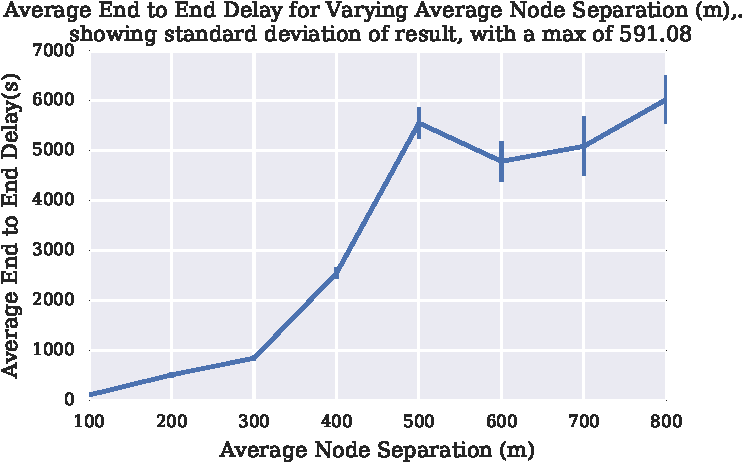
\includegraphics[width=0.6\textwidth]{delay_range}
	\caption{End to End Delay under varying node-separations}
	\label{fig:delay_range}
\end{figure}

\begin{figure}[H]
	\centering
	\missingfigure{rts range}
	%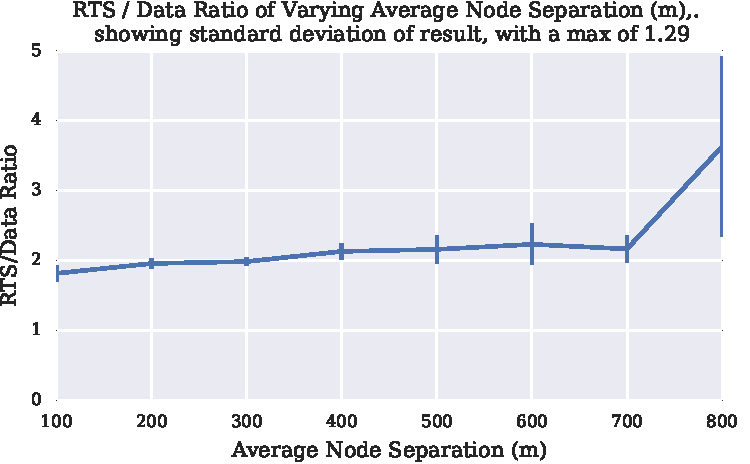
\includegraphics[width=0.6\textwidth]{rts_range}
	\caption{RTS/Data ratio for varying node-separations}
	\label{fig:rts_range}
\end{figure}


\begin{table}[H]
	\caption{Tabular view of data from Figs~\ref{fig:prod_breakdown_range}, \ref{fig:delay_range}, and \ref{fig:rts_range}} \label{tab:rangedelay}
	\begin{center}
		\hyphenpenalty 100000
		\begin{tabular}{
				*{2}{@{\hspace{1em}}r@{\hspace{1em}}}
				*{3}{@{\hspace{1em}}p{0.1\textwidth} @{\hspace{1em}}}  }
			\toprule
			Separation(m) &  Delay(s) &  Probability of Arrival &  RTS/Data Ratio &  Ideal Delivery Time(s) \\
			\midrule
			100 &     60.32 &                    0.99 &            1.80 &                    1.03 \\
			200 &    419.95 &                    0.97 &            2.02 &                    1.10 \\
			300 &   1205.66 &                    0.89 &            2.41 &                    1.17 \\
			400 &   1288.20 &                    0.91 &            2.26 &                    1.25 \\
			500 &   1868.20 &                    0.87 &            2.41 &                    1.32 \\
			600 &   2191.07 &                    0.85 &            2.42 &                    1.39 \\
			\bottomrule
		\end{tabular}
	\end{center}
\end{table}
 % Trust in Autonomous Systems of Systems for Maritime Defence Applications

% !TeX spellcheck = en_GB
\def\ChapterTitle{Strategies for Multi-Domain Trust Assessment}

\ifx\ifthesis\undefined
	\documentclass[a4paper, 11pt]{article}

% % Special Includes stolen from Thesis.cls
\usepackage{booktabs}
\usepackage{hyperref}
\usepackage{graphicx}
\usepackage{epstopdf}
\usepackage{subcaption}
\usepackage{rotating}
\usepackage{listings}
\usepackage{lstpatch}
\renewcommand{\arraystretch}{1.3}

% % % % % % % % % % % % % % % %

% PACKAGES
\usepackage[square, numbers, comma, sort&compress]{natbib}  % Use the "Natbib" style for the references in the Bibliography
\usepackage{verbatim,listings}  % Needed for the "comment" environment to make LaTeX comments
\usepackage{array}  % Needed for the "comment" environment to make LaTeX comments
\usepackage{vector}  % Allows "\bvec{}" and "\buvec{}" for "blackboard" style bold vectors in maths
\usepackage{amsmath,amsfonts,amsthm,color,psfrag,epsf, tabularx, multirow, longtable}
\usepackage{snapshot, todonotes}
% \usepackage{pstricks}
\usepackage{enumerate}
%\usepackage[lined,algonl,boxed]{algorithm2e}
\usepackage[ruled,linesnumbered,vlined]{algorithm2e}
\usepackage{float}
\usepackage{epigraph} % epigraph
\usepackage{tikz}
\usetikzlibrary{shapes.geometric, arrows}

\usepackage{setspace}
\doublespacing
% or:
%\onehalfspacing

% SETUP
\hypersetup{urlcolor=blue, colorlinks=false}  % Colours hyperlinks in blue, but this can be distracting if there are many links. 
\DeclareGraphicsExtensions{.pdf,.jpeg,.png}
\graphicspath{{../Figures/}{../../../Dropbox/Thesis_Figures/}}  % Location of the graphics files (set up for graphics to be in PDF format)

% NOTE THERES A FUCKUP IN TEX4HT http://tug.org/pipermail/tex4ht/2014q2/000944.html
% NEED TO MANUALLY CHANGE \def\pgfsys@svg@newline{{?nl}}
\ifdefined\HCode
\usepackage[compatibility=false]{caption}
\def\pgfsysdriver{pgfsys-tex4ht.def}
\else
\usepackage[]{caption}
\fi

% \SpecialCoor
\def\subsum{\mathit{\Sigma}}

%opening
\title{\ChapterTitle}
\author{Andrew Bolster}

\begin{document}

\maketitle

\else
	\chapter{\ChapterTitle}
	\label{Chapter\thechapter}
	\lhead{Chapter \thechapter. \emph{\nameref{Chapter\thechapter}}} % Write in your own chapter title to set the page header
\fi
 % Strategies for Multi-Domain Trust Assessment

% !TeX spellcheck = en_GB
\def\ChapterTitle{Modelling and Analysis of Collaborative Node Kinematic Behaviours in Underwater Acoustic MANETs}

\ifx\ifthesis\undefined
\documentclass[a4paper, 11pt]{article}

% % Special Includes stolen from Thesis.cls
\usepackage{booktabs}
\usepackage{hyperref}
\usepackage{graphicx}
\usepackage{epstopdf}
\usepackage{subcaption}
\usepackage{rotating}
\usepackage{listings}
\usepackage{lstpatch}
\renewcommand{\arraystretch}{1.3}

% % % % % % % % % % % % % % % %

% PACKAGES
\usepackage[square, numbers, comma, sort&compress]{natbib}  % Use the "Natbib" style for the references in the Bibliography
\usepackage{verbatim,listings}  % Needed for the "comment" environment to make LaTeX comments
\usepackage{array}  % Needed for the "comment" environment to make LaTeX comments
\usepackage{vector}  % Allows "\bvec{}" and "\buvec{}" for "blackboard" style bold vectors in maths
\usepackage{amsmath,amsfonts,amsthm,color,psfrag,epsf, tabularx, multirow, longtable}
\usepackage{snapshot, todonotes}
% \usepackage{pstricks}
\usepackage{enumerate}
%\usepackage[lined,algonl,boxed]{algorithm2e}
\usepackage[ruled,linesnumbered,vlined]{algorithm2e}
\usepackage{float}
\usepackage{epigraph} % epigraph
\usepackage{tikz}
\usetikzlibrary{shapes.geometric, arrows}

\usepackage{setspace}
\doublespacing
% or:
%\onehalfspacing

% SETUP
\hypersetup{urlcolor=blue, colorlinks=false}  % Colours hyperlinks in blue, but this can be distracting if there are many links. 
\DeclareGraphicsExtensions{.pdf,.jpeg,.png}
\graphicspath{{../Figures/}{../../../Dropbox/Thesis_Figures/}}  % Location of the graphics files (set up for graphics to be in PDF format)

% NOTE THERES A FUCKUP IN TEX4HT http://tug.org/pipermail/tex4ht/2014q2/000944.html
% NEED TO MANUALLY CHANGE \def\pgfsys@svg@newline{{?nl}}
\ifdefined\HCode
\usepackage[compatibility=false]{caption}
\def\pgfsysdriver{pgfsys-tex4ht.def}
\else
\usepackage[]{caption}
\fi

% \SpecialCoor
\def\subsum{\mathit{\Sigma}}

%opening
\title{\ChapterTitle}
\author{Andrew Bolster}

\begin{document}

\maketitle

\else
\chapter{\ChapterTitle}
\label{Chapter\thechapter}
\lhead{Chapter \thechapter. \emph{\nameref{Chapter\thechapter}}} % Write in your own chapter title to set the page header
\fi




\section{Introduction}\label{sec:introduction}
% no \IEEEPARstart
% You must have at least 2 lines in the paragraph with the drop letter
% (should never be an issue)

As mobile ad-hoc networks (MANETs) grow beyond the terrestrial arena, their operation and the protocols designed around them must be reviewed to assess their suitability to different communications environments to ensure their continued security, reliability, and performance.

One area of application is the underwater marine environment, where extreme challenges to communications present themselves (propagation delays, frequency dependent attenuation, fast and slow fading, refractive multi-path distortion, etc.).
In addition to the communications challenges, other considerations such as command and control isolation, as well as power and locomotive limitations, drive towards the use of teams of smaller and cheaper autonomous underwater vehicles (AUVs). 
These increasingly decentralised applications present unique threats against trust management \cite{Caiti2011}.
In underwater environments, communications is both sparse and noisy.
Therefore the observations about the communications processes that are used to generate the trust metrics, occur much less frequently, with much greater error (noise) and delay than is experienced in terrestrial RF MANETS.
As such, the use of trust methods developed in the terrestrial MANET space must be re-appraised for application within the underwater context \cite{Pavan2015}.

Trust Management Frameworks (TMFs) provide information to assist the estimation of future states and actions of nodes within networks.
This information is used to optimize the performance of a network against malicious, selfish, or defective misbehaviour by one or more nodes.
Previous research has established the advantages of implementing TMFs in 802.11 based MANETs, particularly in terms of preventing selfish operation in collaborative systems \cite{Li2007}, and maintaining throughput in the presence of malicious actors \cite{Buchegger2002}

Most current TMFs use a single type of observed action to derive trust values, typically successfully delivered or forwarded packets. 
These observations then inform future decisions of individual nodes, for example, route selection \cite{Li2008}.

Recent work has demonstrated the use of a number of metrics to form a ``vector'' of trust.
The Multi-parameter Trust Framework for MANETs (MTFM) \cite{Guo11}, uses a range of communications metrics beyond packet delivery/loss rate (PLR) to assess trust.
This vectorized trust also allows a system to detect and identify the tactics being used to undermine or subvert trust.
To date this work has been limited to terrestrial, RF based networks. 

The paper is laid out as follows.
In Section \ref{sec:trustandtmfs} we discuss Trust and TMFs, defining our terminology and reviewing the justifications for the use and development of TMFs for marine acoustic networks (MANs)
In Section \ref{sec:marineacousticnetworks} we review selected features of the underwater communications channel, highlighting particular challenges against terrestrial equivalents.
In Section \ref{sec:initialsystemcharacterization} we establish an experimental configuration for the marine space, and review the scenarios and results presented in \cite{Guo11}.
In Section \ref{sec:trustresultsanddiscussion} we present our findings in trust establishment and malicious behaviour detection, comparing with other current TMFs (Hermes and OTMF) and analyse the use of this multi-parameter approach to detecting malicious and selfish behaviour in autonomous marine networks.

The contributions of this paper are a study on the comparative operation and performance of TMFs in marine acoustic networks, and a review of metric suitability for TMFs in marine environments, informing future metric selection for experimenters and theorists.
We also show that single metric trust systems are not directly suitable for the marine context in terms of the different threat and cost scenario in that environment.
Finally, we demonstrate a methodology to assess the usefulness of metrics in discriminating against misbehaviours in such constrained, delay-tolerant networks.



\section{Trust and Trust Management Frameworks}\label{sec:trustandtmfs}


\subsection{Trust in Conventional MANETs}\label{sec:trustinmanets}

The distributed and dynamic nature of MANETs mean that it is difficult to maintain a trusted third party (TTP) or evidence based trust system such as Certificate Authorities (CA) or Public Key Infrastructure (PKI).
Distributed trust management frameworks aim to detect, identify, and mitigate the impacts of malicious actors by distributing per-node assessments and opinions to collectively police behaviour.
Various models and algorithms for describing trust and developing trust management in distributed systems, P2P communities or wireless networks have been considered.
\emph{Hermes Trust Establishment Framework} takes a Bayesian Beta function to model per-link Packet Loss Rate (PLR) over time, combining ``Trust'' and ``Confidence of Assessment'' into a single value \cite{Zouridaki2005}.
\emph{Objective Trust Management Framework} (OTMF) builds upon Hermes and distributes node observations across the network \cite{Li2008}, however does not appropriately combat multi-node-collusion in the network \cite{Cho2011}.
\emph{Trust-based Secure Routing} demonstrated an extension to Dynamic Source Routing (DSR), incorporating a Hidden Markov Model of sub-networks, reducing the efficacy of Byzantine attacks such as black-hole routing  \cite{Moe2008a}.
\emph{CONFIDANT} presented an approach using a probabilistic estimation of PLR, similar to OTMF, also introducing a topology aware weighting scheme and also weighting trust assessments based on historical experience of the reporter \cite{Buchegger2002}.
\emph{Fuzzy Trust-Based Filtering} uses Fuzzy Inference to adapt to malicious recommenders using conditional similarity to classify performance with overlapping fuzzy set membership, filtering assessments across a network \cite{Luo2008}. 

These TMFs can be generalised as single-value estimation based on a binary input state (success or failure of packet delivery) and generating a probabilistic estimation of the future states of that input. 

These single metric TMFs provide malicious actors with a significant advantage if their activity does not impact that metric.
In the case where the attacker can subvert the TMF, the metric under assessment by that TMF does not cover the threat mounted by the attacker.
This causes a significant negative effect on the efficiency of the network, as the TMF is assumed to have reduced the possible set of attacks when it has actually made it more advantageous to attack a different part of the networks operation.
An example of such a situation would be in a TMF focused on PLR where an attacker selectively delays packets going through it, reducing overall throughput but not dropping any packets.
Such behaviour would not be detected by the TMF.

For the purposes of this work, we select Hermes trust establishment and OTMF as indicative single-metric TMFs to compare against MTFM, as Hermes captures the core operation of a pure single metric assessment methodology and OTMF provides a comparison that combines assessments from across nodes to develop trust opinions.


\subsection{Trust in Marine Networks}\label{sec:trust_in_marine}

With demand for smaller, more decentralised marine survey and monitoring systems, and a drive towards lower per-unit cost, pressures on battery capacity, locomotive power efficiency, data processing and storage are increasing.
These pressures simultaneously present opportunities and incentives for malicious or selfish actors to appear to cooperate while not reciprocating, in order to conserve power for instance.

Within UANs observable metrics include significant noise and may occur at irregular and sparse intervals.
Conventional approaches such as probabilistic estimation do not produce trust values that reflect the underlying reality and context of the metrics available, as they require a-priori assumption that the trust value under exploration has an expected distribution, that distribution is mono-modal, and the input metrics are binary.
In scenarios with variable, sparse, noisy metrics, estimating the distribution is difficult to accomplish a-priori.

\subsection{Single Metric Trust Frameworks}

The Hermes trust establishment framework \cite{Zouridaki2005} uses Bayesian reasoning to generate a posterior distribution function of ``belief'', or trust, given a sequence of observations of that behaviour, $p(B|O)$\eqref{eq:otmf_pbo}.

\begin{equation}
	p(B|O)  = \frac{p(O|B) \times p(B)}{\rho}
	\label{eq:otmf_pbo}
\end{equation}

Where $p(B)$ is the prior probability density function for the expected normal behaviour, and $\rho$ is a normalising factor.
Due to it's flexibility and simplicity, Hermes assumes that $p(B)$ is a Beta function, and therefore the evaluation of this trust assessment is based around the expectation value of the distribution \eqref{eq:otmf_t}  where $\alpha$ and $\beta$ represent the number of successful and unsuccessful interactions respectively for a particular node $i$.

A secondary measurement of the confidence factor of the trust assessment $t$ is generated as \eqref{eq:otmf_c} and these measurements are combined to form a ``trustworthiness'' value $T$ \eqref{eq:otmf_trust}.

\begin{align}
	t_i &\to E\lbrack\text{beta}(p|\alpha,\beta)\rbrack = \frac{\alpha_i}{\alpha_i+\beta_i} \label{eq:otmf_t}\\[5pt]
	c_i &= 1 - \sqrt{\frac{12\alpha_i\beta_i}{(\alpha_i+\beta_i)^2(\alpha_i+\beta_i+1)}} \label{eq:otmf_c}\\[5pt]
	T_i &= 1 - \frac{\sqrt{\frac{(t_i-1)^2}{x^2} + \frac{(c_i-1)^2}{y^2}}}{\sqrt{\frac{1}{x^2}+\frac{1}{y^2}}} \label{eq:otmf_trust}
\end{align}

In \eqref{eq:otmf_trust}, $x$ and $y$ are constants, used weight the two-dimensional polar mapping of trust and confidence assessments ($t_i,c_i$), and from \cite{Zouridaki2005}, are taken as $x=\sqrt{2},y=\sqrt{9}$.

Upon this per-node assessment methodology, OTMF overlays an observation distribution protocol so as to make the measurements $\alpha_i$ and $\beta_i$ representative of the direct and 1-hop networks observations of the target node $i$, as well as expiring old observations from assessment and eliminating observations from ``untrustworthy'' nodes.


\subsection{Multi-Metric Trust Frameworks}\label{sec:multimetrictrust}

Given the potential incentives to a selfish attacker and potential threats to trust and fairness in sparse, noisy, and constrained environments, single metric trusts discussed above do not suitably cover the exposed threat surface. 
This indicates that a multi-metric approach may be more appropriate to capture and monitor the realities of an environment such as those experienced by UANs.

Grey Theory performs cohort based normalization of metrics at runtime, providing a ``grade'' of trust compared to other observed nodes in that interval, while maintaining the ability to reduce trust values down to a stable assessment range for decision support without requiring every environment entered into to be characterised.
This presents a stark difference between the Grey and Probabilistic approaches.
Grey assessments are relative in both fairly and unfairly operating networks.
All nodes will receive mid-range trust assessments if there are no malicious actors as there is nothing ``bad'' to compare against, and variations in assessment will be primarily driven by topological and environmental factors.
Guo et al. \cite{Guo11} demonstrated the ability of grey relational analysis (GRA) \cite{Zuo1995} to normalise and combine disparate traits of a communications link such as instantaneous throughput, received signal strength, etc. into a grey relational coefficient (GRC), or a ``trust vector'' in this instance.

The grey relational vector is given as
%
\begin{align}
	\label{eq:grc}
	\theta_{k,j}^t = \frac{\min_k|a_{k,j}^t - g_j^t| + \rho \max_k|a_{k,j}^t-g_j^t|}{|a_{k,j}^t-g_j^t| + \rho \max_k|a_{k,j}^t-g_j^t|} \\
	\phi_{k,j}^t = \frac{\min_k|a_{k,j}^t - b_j^t| + \rho \max_k|a_{k,j}^t-b_j^t|}{|a_{k,j}^t-b_j^t| + \rho \max_k|a_{k,j}^t-b_j^t|} \notag 
\end{align}
%
where $a_{k,j}^t$ is the value of an observed metric $x_j$ for a given node $k$ at time $t$, $\rho$ is a distinguishing coefficient set to $0.5$, $g$ and $b$ are respectively the ``good'' and ``bad'' reference metric sequences from $\{a_{k,j}^t k=1,2\dots K\}$, i.e. $g_j=\max_k({a_{k,j}^t})$,  $b_j=\min_k({a_{k,j}^t})$ (where each metric is selected to be monotonically positive for trust assessment, e.g. higher throughput is presumed to be always better). 

Weighting can be applied before generating a scalar value \eqref{eq:metric_weighting} allowing the detection and classification of misbehaviours.

%
\begin{equation}
	\label{eq:metric_weighting}
	[\theta_k^t, \phi_k^t] = \left[\sum_{j=0}^M h_j \theta_{k,j}^t,\sum_{j=0}^M h_j \phi_{k,j}^t \right]
\end{equation}
%
Where $H=[h_0\dots h_M]$ is a metric weighting vector such that $\sum h_j = 1$, and in unweighted case, $H=[\frac{1}{M},\frac{1}{M}\dots\frac{1}{M}]$.
$\theta$ and $\phi$ are then scaled to $[0,1]$ using the mapping $y = 1.5 x - 0.5$.
To minimise the uncertainties of belonging to either best ($g$) or worst ($b$) sequences in \eqref{eq:grc} the $[\theta,\phi]$ values are reduced into a scalar trust value by $T_k^t = ({1+{(\phi_k^t)^2}/{(\theta_k^t)^2}})^{-1}$ \cite{Hong2010}.
MTFM combines this GRA with a topology-aware weighting scheme \eqref{eq:networkeffects} and a fuzzy whitenization model \eqref{eq:whitenization}. 

There are three classes of topological trust relationship used; Direct, Recommendation, and Indirect.
Where an observing node $n_i$ assesses the trust of another target node, $n_j$; the Direct relationship is $n_i$'s own observations $n_j$'s behaviour.
In the Recommendation case, a node $n_k$ which shares Direct relationships with both $n_i$ and $n_j$, gives its assessment of $n_j$ to $n_i$.
In the Indirect case, similar to the Recommendation case, the recommender $n_k$ does not have a direct link with the observer $n_i$ but $n_k$ has a Direct link with the target node, $n_j$.
These relationships give node sets, $N_R$ and $N_I$ containing the nodes that have recommendation or indirect, relationships to the observing node respectively.
%
\begin{align}
	\label{eq:networkeffects}
	T_{i,j}^{MTFM}=&\frac{1}{2} \cdot \max_s\{f_s(T_{i,j})\} T_{i,j}\\ \notag
	+&\frac{1}{2} \frac{2|N_R| }{2|N_R| + |N_I|}\sum_{n \in N_R} \max_s\{f_s(T_{i,n})\} T_{i,n}\\ \notag
	+&\frac{1}{2} \frac{|N_I| }{2|N_R| + |N_I|}\sum_{n \in N_I} \max_s\{f_s(T_{i,n})\} T_{i,n} 
\end{align}

Where $T_{i,n}$ is the subjective trust assessment of $n_i$ by $n_n$, and $f_s = [ f_1,f_2, f_3]$ given as:

\begin{align}
	\label{eq:whitenization}
	f_1(x)&= -x+1\notag\\
	f_2(x)&= 
	\begin{cases}
		2x & \text{if }x\leq 0.5\\
		-2x+2 & \text{if }x>0.5
	\end{cases}\\
	f_3(x)&= x\notag
\end{align}
%
In the case of the terrestrial communications network used in \cite{Guo11}, the observed metric set $X = {x_1,\dots,x_M}$ representing the measurements taken by each node of its neighbours at least interval, is defined as $X=[$packet loss rate, signal strength, data rate, delay, throughput$]$.

Guo et al. demonstrated that when compared against OTMF and Hermes trust assessment, MTFM provided increased variation in trust assessment over time, providing more information about the nodes' behaviours than packet delivery probability alone can.

By weighting the metrics used in MTFM it was shown that the trust assessments could be used to identify the style of misbehaviour being performed within the network, and by whom.
We present a corollary method to investigate and apply this work to the Marine MANET field.


\section{Marine Acoustic Communications}\label{sec:marineacousticnetworks}

The key challenges of underwater acoustic communications are centred around the impact of slow and differential propagation of energy (RF, Optical, Acoustic) through water, and its interfaces with the seabed / air.
The resultant challenges include; long propagation delays, significant inter-symbol interference and Doppler spreading, fast and slow fading due to environmental effects (aquatic flora/fauna, surface weather), carrier-frequency dependent signal attenuation, multi-path caused by reflective medium interfaces, variations in propagation speed due to depth dependant effects (salinity, temperature, and pressure), and subsequent refractive spreading and lensing due to that same propagation variation \cite{Partan2006}.

The attenuation that occurs in an underwater acoustic channel over a distance $d$ for a signal about frequency $f$ in linear power is given as $A_{\text{aco}}(d,f) = A_0d^ka(f)^d$ and in $dB$ form as;
%
\begin{equation}
	\label{eq:acoattenuationdb}
	10 \log A_{\text{aco}}(d,f)/A_0 = k \cdot 10 \log d + d \cdot 10 \log a(f)
\end{equation}
%
where $A_0$ is a normalising constant, $k$ is a spreading factor (commonly taken as 1.5  \cite{Stojanovic2007}), and $a(f)$ is the absorption coefficient, approximated using Thorp's formula \cite{Stefanov2011}
%
\begin{equation}
	\label{eq:thorp}
	10 \log a(f) = \frac{0.11 \cdot f^2}{1+f^2} + \frac{44\cdot f^2}{4100+f^2}+ 2.75\times10^{-4} f^2 + 0.003
\end{equation}
%
Refractive lensing and the multi-path nature of the medium result in line of sight propagation being extremely unreliable for estimating distances to targets.
The first arriving acoustic signal has as the very least curved in the medium, and commonly has reflected off the surface/seabed before arriving at a receiver, creating secondary paths that are sometimes many times longer than the first arrival path, generating symbol spreading over orders of seconds depending on the ranges and depths involved.
Forward Error Correction coding is used on such channels to minimise packet losses.

Comparing $A_{aco}(d,f)$ with the RF Free-Space Path Loss model $(A_{\text{RF}}(d,f) \approx \left( \frac{4\pi d f}{c} \right)^2)$, the impact of range on signal power is exponential underwater, rather than quadratic in terrestrial RF ($A_{\text{aco}} \propto f^{2d}$ vs $A_{\text{RF}} \propto (df)^2$). 
While both frequency dependant factors are quadratic, approximating the factors in \eqref{eq:thorp}, $f\propto A_{\text{aco}}$ is at least 4 orders of magnitude higher than $f\propto A_{\text{RF}}$



\section{System Model Characterization}\label{sec:initialsystemcharacterization}


\subsection{Mobility, Topology, and Communications}

We apply two mobility patterns for investigation; all nodes static and all nodes mobile.
The reason for this is that in other mobility combinations, the node targeted for misbehaviour ($n_1$) will already be behaving differently compared to the rest of the network regardless of the misbehaviour.

The six nodes are initially arranged as per Fig.~\ref{fig:s1_layout} with each node on average 100m from each other as per \cite{Guo11}.
The use of six nodes and the particular layout enables the investigation of the three trust relationships based on minimum path topologies, such that the node generating the trust assessments, $n_0$ has Direct, Recommendation, and Indirect trust assessments of $n_1$ available to it from itself, $[n_2,n_3]$, and $[n_4,n_5]$ respectively. 

Collaborations with NATOs Centre for Maritime Research and Experimentation (CMRE) in La Spezia, and DSTLs Naval Systems Group inform that this is a practical team-size for environmental and defence applications.

%
\begin{figure}[h]
	\centering
	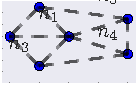
\includegraphics[width=.45\textwidth]{s1_layout}
	\caption{Initial layout with nodes spaced an average of 100m apart}
	\label{fig:s1_layout}
\end{figure}
%

\subsection{Simulation Background}

Simulations were conducted using a Python based simulation framework, SimPy \cite{Mueller2003SimPy}, with a network stack built upon AUVNetSim \cite{Miquel2008}, with transmission parameters (Table \ref{tab:sysconstraints}) taken from and validated against \cite{Stojanovic2007} and \cite{Stefanov2011}.

Given the differences in delay and propagation between RF and marine networks, it would not be expected that the same application rates (e.g. packet emission rates or throughput) and node separations are equally stable in this environment.
Therefore, we first characterise a zone of performance within which the network have stable operation.
%
\begin{table}[h]
	\caption{Comparison of system model constraints as applied between Terrestrial and Marine communications} \label{tab:sysconstraints}
	\begin{center}
		\setlength{\tabcolsep}{8pt}
		\begin{tabular}{lccc}
			\toprule
			Parameter & Unit & Terrestrial & Marine \\
			\midrule
			Simulated Duration & $s$ & 300 & 18000\\
			Trust Sampling Period & $s$ & 1 & 600 \\
			Simulated Area & $km^2$ & 0.7 & 0.7-4 \\
			Transmission Range & $km$ & 0.25 & 1.5 \\
			Physical Layer & & RF(802.11) & Acoustic\\
			Propagation Speed& $m/s$ & $3\times10^8$ & 1490\\
			Center Frequency& $Hz$ & $2.6\times10^9$ & $2 \times 10^4$ \\
			Bandwidth& $Hz$ & $22\times10^6$ & $1\times10^4$\\
			MAC Type & & CSMA/DCF & CSMA/CA\\
			Routing Protocol & & DSDV & FBR \\
			Max Speed & $ms^{-1}$ & 5 & 1.5 \\
			Max Data Rate & $bps$ & $5\times10^6$ & $\approx 240$ \\
			Packet Size & bits & 4096 &  9600 \\
			Single Transmission Duration & $s$ & 10 & 32 \\
			Single Transmission Size & bits & $10^7$ & $9600$ \\
			\bottomrule
		\end{tabular}
		\setlength{\tabcolsep}{6pt}
	\end{center}
\end{table}
%


\subsection{Scaling Considerations between Terrestrial and Underwater Environments}

We establish an appropriate safe operating zone for marine communications by looking at the communications rate and physical distribution factors across the two selected mobility scenarios.
From Table~\ref{tab:sysconstraints}, the operating transmission range of this model of acoustic communications is $\approx 6$ times further than that of 802.11, indicating that a suitable operating environment will have an area $\approx \sqrt{6}$ times the area of the 802.11 case.
However, it was recognised in Section~\ref{sec:marineacousticnetworks} that underwater, the relationship between attenuation and distance is exponential, so this would represent an upper bound of performance, where nodes are approximately 400m apart. 

Exploratory simulations were run to further constrain this bound.
As the separation is increased, the emission rate at which the network becomes saturated decreases, reducing overall throughput. 
This throughput degradation is tightly coupled with the mobility, as increasing mobility leads to increasing delays as routes are constantly broken, re-advertised and re-established. 
For instance, where all nodes are static, we do not see significant drops in saturation rates until node separation approaches 800m, nearly double the initial estimate. 
When all nodes are randomly walking the saturation point collapses from 0.025pps at 300m to 0.015pps at 400m.
Our results indicate that the best area to continue operating in for a range of node separations is at 0.015pps, and that a reasonable position scaling is from 100m to 300m, beyond which communication becomes increasingly unstable, especially in terms of end-to-end delay.
These results are similar to work performed in \cite{Miquel2008}, and are expected in such a sparse, noisy, and contentious environment. 


\subsection{Selected Misbehaviours}


We are primarily concerned with the direct trust relationship between $n_0$ and $n_1$, i.e. $n_0$'s assessment of the trustworthiness of $n_1$, or $T_{1,0}$.

Guo et al. introduce a range of misbehaviours, including modification of the packet loss rate of routing nodes and limiting throughput on a per-link basis as well as a selection of combined misbehaviours. 
Given that the established links are already heavily constrained, such attacks would severely impact the general performance of the network beyond the scope of simple selfishness.
These direct malicious behaviours effectively trigger saturation collapses in operating regions of the network that should be stable.

Therefore, we apply two more subtle misbehaviours to investigate; 
\begin{enumerate}
	\item Malicious Power Control (MPC), where $n_1$ increases its transmit and forwarding power by 20\% for all nodes \emph{except} communications from $n_0$ in order to make $n_0$ appear to be selfishly conserving energy to the rest of the team, while $n_1$ itself appears to be performing very well.
	\item Selfish Target Selection (STS), where $n_1$ preferentially communicates, forwards and advertises to nodes that are physically close to it in effort to reduce its own power consumption.
\end{enumerate}


\section{Simulation Results and Discussion}\label{sec:trustresultsanddiscussion}

Having established a safe operating range for comparison at 300m average separation and an emission rate of 0.015pps, we perform each of the three selected behaviours (Fair, MPC, STS) in both the static and mobile scenarios. 
We select a trust assessment period of 10 mins for a 5 hour mission to scale in comparison to relative bitrates experienced (1Mbps vs $\approx15$bps).

The six metrics used for grey assessment are; transmitted and received throughput and power, delay, and packet loss rate (PLR) as calculated by aborted and unacknowledged, transmissions.
Compared to \cite{Guo11}, this metric set lacks a data rate quantity as the network is not dynamically adjusting bandwidth.
In context of GRC generation \eqref{eq:grc}, the best sequence $g$ was selected using the lowest PLR, delay, and powers, and the highest throughputs, and the worst sequence, $b$ the inverse of these metrics, reflecting the observations made in Section~\ref{sec:trust_in_marine}.

The particular factors under discussion are the relative performance of MTFM against OTMF and Beta with respect to statistical stability across mobilities and in responsiveness to changing network behaviour. 
We establish a similar result set by initially tracking the resultant trust values established by MTFM in the pair of mobility scenarios, shown in Fig.~\ref{fig:trust_mobility}.
We are also concerned with the opinions of $n_1$ provided to $n_0$ by other nodes, where $[T_{1,2},T_{1,3}]$ and $[T_{1,4},T_{1,5}]$ denote the sets of recommendation and indirect trust assessment respectively.

We also include aggregate assessments; $T_{1,\text{Avg}}$, the unweighted mean of direct trust assessments of $n_1$ from all nodes and $T_{1,\text{MTFM}}$, the final MTFM trust assessment value based on both network topology and whitenization from \eqref{eq:whitenization}.

The variability in assessment is coupled to mobility; in the static case (Fig.~\ref{fig:trust_static}), we see that the nodes exhibit relatively consistent distributions.
In the full mobility case, shown in Fig.~\ref{fig:trust_all_mobile}, this subjective variability is greatly increased. 
As the topology is highly dynamic, delays due to re-establishing routes can be very large, perturbing the trust value.
The $T_{1,\text{MTFM}}$ displays a significantly reduced variation than those of the individual subjective observations in all cases, even when compared to the unweighted average, $T_{1,\text{Avg}}$.
This demonstrates $T_{MTFM}$'s value as an aggregating trust assessment in such sparse and noisy environments.
Further, in Fig.~\ref{fig:trust_all_mobile_mal} we observe a much higher variability in assessment in $T_0$, correctly indicating that there is something wrong with the relationship between $n_0$ and $n_1$.

\begin{figure}[h]
	\centering
	\begin{subfigure}{0.5\textwidth}
	\caption{Fair Static}
	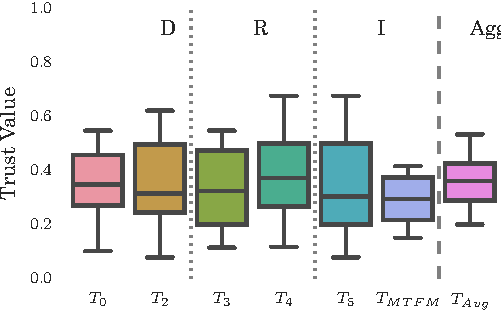
\includegraphics[width=\linewidth]{trust_bella_static_fair} 
	\label{fig:trust_static}
	\end{subfigure}%
	\begin{subfigure}{0.5\textwidth}
	\caption{Fair Mobile}
	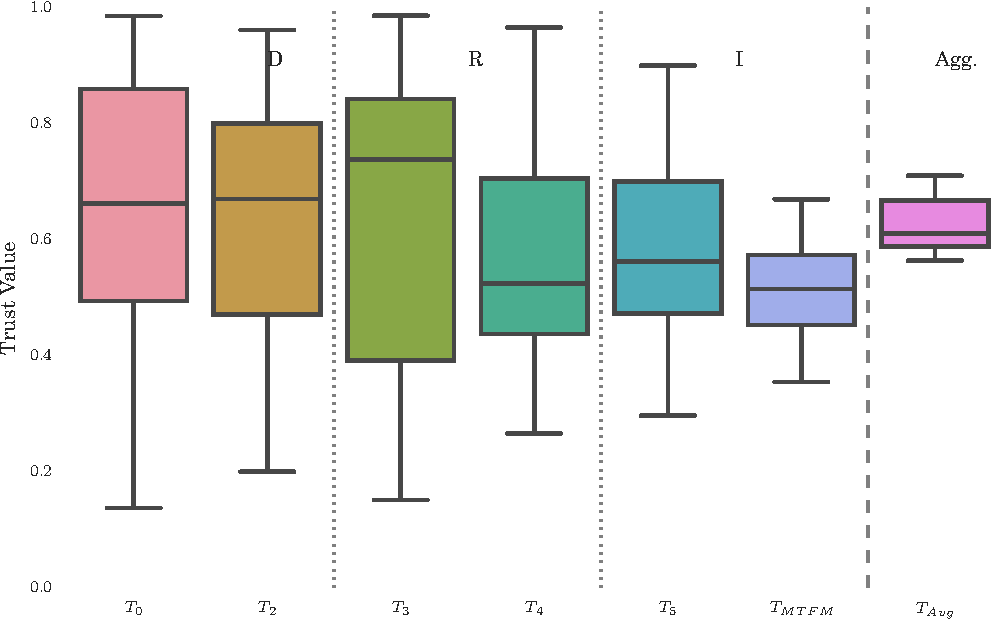
\includegraphics[width=\linewidth]{trust_bella_all_mobile_fair}  
	\label{fig:trust_all_mobile}
	\end{subfigure}%
	
	\begin{subfigure}{0.5\textwidth}
	\caption{Malicious Static}
	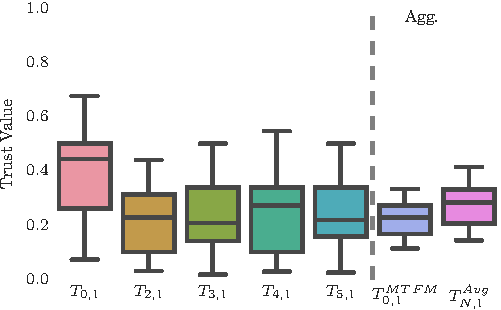
\includegraphics[width=\linewidth]{trust_bella_static_malicious} 
	\label{fig:trust_static_mal}
	\end{subfigure}%
	\begin{subfigure}{0.5\textwidth}
	\caption{Malicious Mobile}
	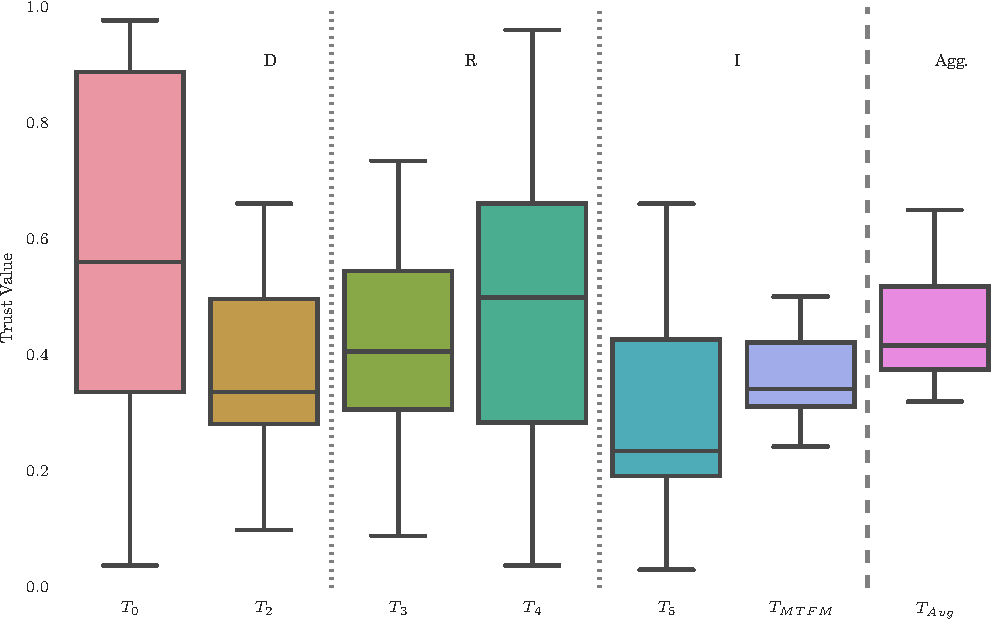
\includegraphics[width=\linewidth]{trust_bella_all_mobile_malicious}  
	\label{fig:trust_all_mobile_mal}
	\end{subfigure}%
	
	\begin{subfigure}{0.5\textwidth}
	\caption{Selfish Static}
	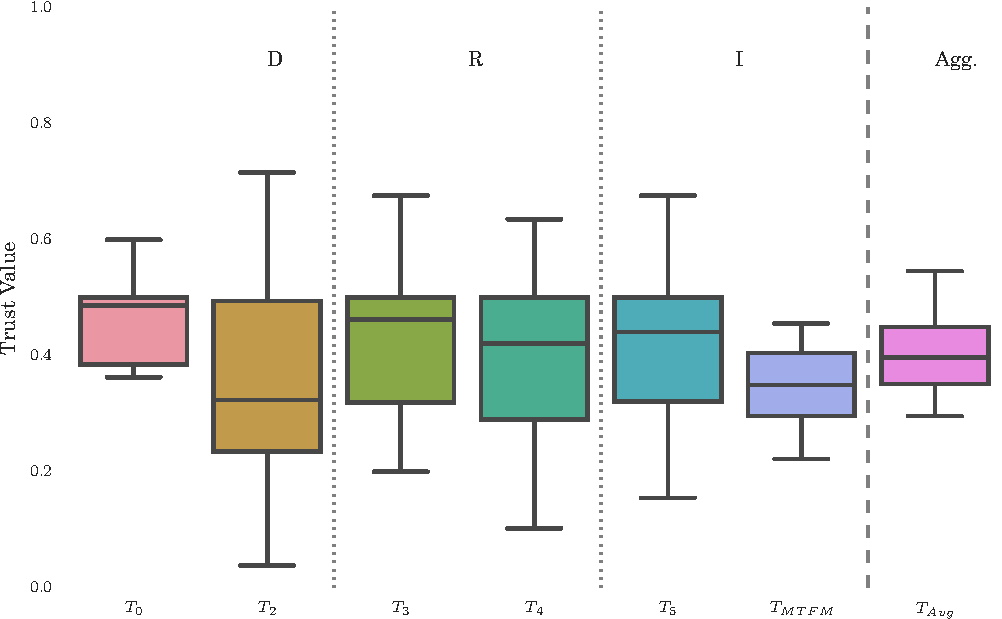
\includegraphics[width=\linewidth]{trust_bella_static_selfish}
	\label{fig:trust_static_sel}
	\end{subfigure}%
	\begin{subfigure}{0.5\textwidth}
	\caption{Selfish Mobile}
	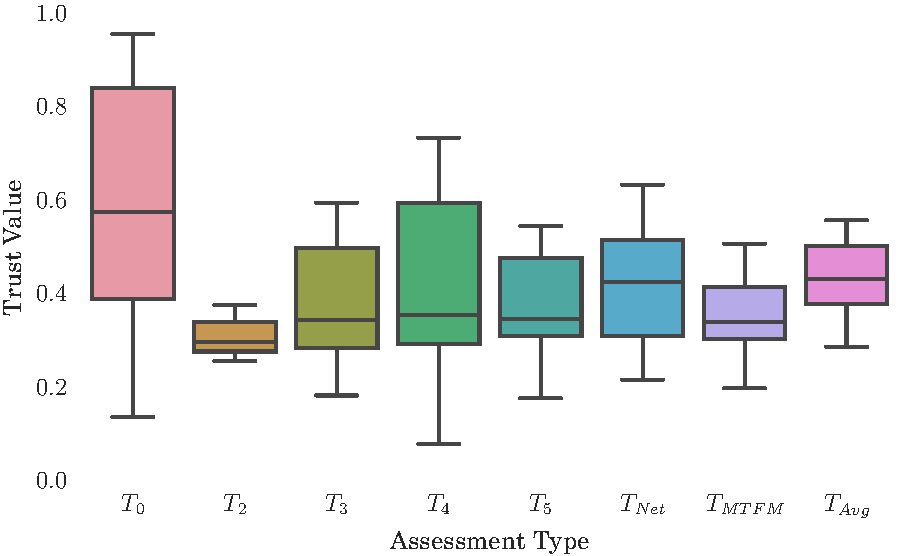
\includegraphics[width=\linewidth]{trust_bella_all_mobile_selfish}  \label{fig:trust_all_mobile_sel}
	\end{subfigure}%

	\caption{MTFM Trust assessments of $n_1$ ($T_{1,X}$), showing Direct, Recommender and Indirect relationships, as well as the Aggregate trust assessments from combining these} 
	\label{fig:trust_mobility}
\end{figure}
%

\subsection{Comparison between MTFM, Hermes and OTFM}
As per \cite{Guo11}, ``fair'' scenarios were also performed with no malicious behaviour, applying OTMF and Hermes assessment as well as MTFM, providing like-for-like comparison of assessment.
For simplicity of presentation, we only consider the fully-mobile scenario, as we are concerned with the establishment of trust in mobile networks

\begin{figure*}[t]
	\begin{subfigure}{0.32\textwidth}	
	\caption{Fair Scenario}
	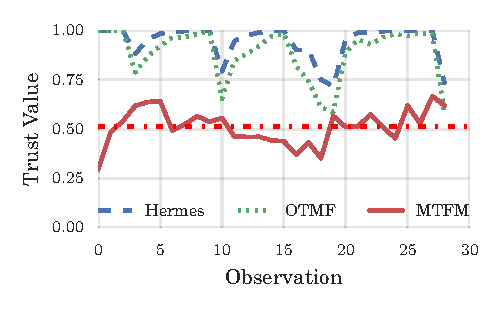
\includegraphics[width=\linewidth]{trust_beta_otmf_fair}
	\label{fig:all_mobile_fair_beta}
	\end{subfigure}
	\begin{subfigure}{0.32\textwidth}
	\caption{Malicious Power Control Scenario}
	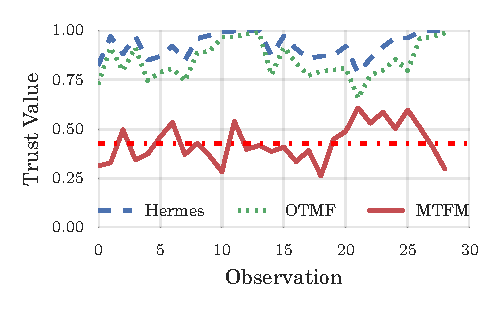
\includegraphics[width=\linewidth]{trust_beta_otmf_malicious} 
	\label{fig:all_mobile_badmouthing_beta}
	\end{subfigure}
	\begin{subfigure}{0.32\textwidth}	
	\caption{Selfish Target Selection Scenario}
	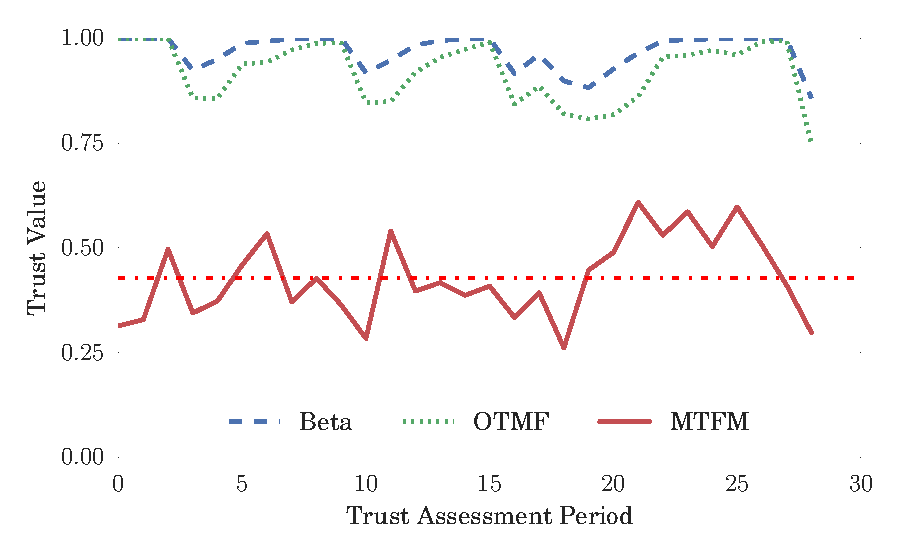
\includegraphics[width=\linewidth]{trust_beta_otmf_selfish} 
	\label{fig:all_mobile_selfish_beta}
	\end{subfigure}
	\caption{$T_{1,0}$ for Hermes, OTMF and MTFM assessment values for fair and malicious behaviours in the fully mobile scenario (mean of MTFM also shown)}
	\label{fig:otmf_beta_comparison}
\end{figure*}
%
The use of Forward Beam Routing and a CSMA/CA MAC scheme from AUVNetSim \cite{Miquel2008} in our simulation mitigates a significant number of packet losses through collision avoidance and contention handling, leading to the situation that the only genuinely lost packets occur when a node moves completely out of range of any other node and time out occurs in route discovery rather than transmission.
As such, confirmed packet losses are relatively rare and in a delaying network like this, it is difficult to set a differentiating time out between packets that are in the network but queued, and packets that are actually ``lost''.

The single metric TMFs used in conventional MANETs require regular and constant input to shape and adjust their evaluations, which for a network with significant and irregular delays such as this, is not practical.
This renders OTMF and Hermes assessment at best uninformative and at worst misleading; consistently providing nodes a high trust assessment as they have very little information to extract trust from. 

Fig.~\ref{fig:otmf_beta_comparison} shows a comparison between the unweighted response of MTFM compared to OTMF and Hermes assessment functions on the same data for the fair, malicious and selfish behaviours respectively.
It is important to note a distinction between the expectations of MTFM compared to other TMFs; MTFM is primarily concerned with the identification of differences in the behaviours of nodes in a network, and is relative rather than absolute.
That is to say that under MTFM, nodes are compared against the worst current performances across metrics of other observed nodes and graded against them, rather than the absolute (objective) approach taken by many TMFs.
In these cases, particularly since the methods of attack were not directly related to PLR, OTMF and Hermes have not registered significant activity in either misbehaviour when compared to the fair scenario.
The difference between the MTFM trust assessments under ``fair'' and ``malicious'' behaviour is lowered by $\approx 10\%$ in both cases, in terms of the mean values returned.
At run time, similar results could be attained by an exponentially weighted moving average filter (EWMA).

On their own, neither OTMF, Hermes, or unbiased MTFM appear to be effective in detecting or identifying malicious behaviour in this environment, in fact OTMF and Hermes don't appear to differentiate between fair and selfish scenarios at all.


\subsection{Metric Weighting}
%

We apply a sequence of vectors that preferentially weight each metric in Eq. \eqref{eq:metric_weighting} to each of the three simulation runs.
For a metric weight vector $H$, where the metric $m_j$ is emphasised as being twice as important as the other metrics, we form an initial weighting vector $H'=[h_i...h_M]$ such that $h_i = 1 \forall i \ne j; h_j=2$. We then scale that vector $H'$ such that $\sum H = 1$ by $H= \frac{H'}{\sum H'}$.
Using this process we can extract and highlight the primary aspects of an attack by comparing against the deviation from the ``fair'' result set. 

\begin{figure}[h]
	\centering
	\begin{subfigure}{0.5\textwidth}
		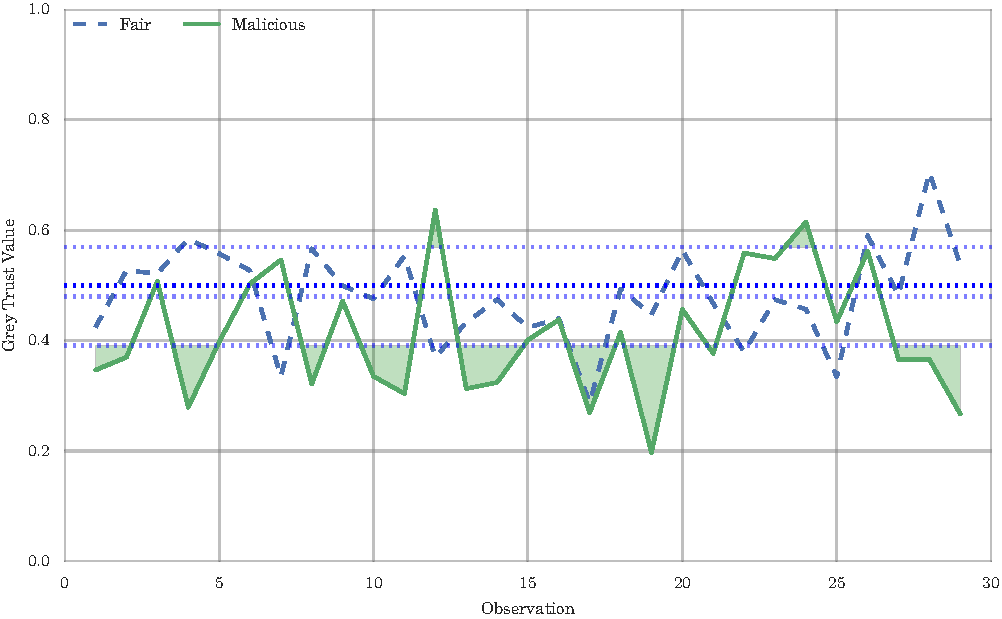
\includegraphics[width=.45\linewidth]{trust_bella_all_mobile_emph_ADelay_BadMouthingPowerControl} \label{fig:all_mobile_badmouthing_delay}
		\caption{Delay Emphasised}
	\end{subfigure}
	\begin{subfigure}{0.5\textwidth}
		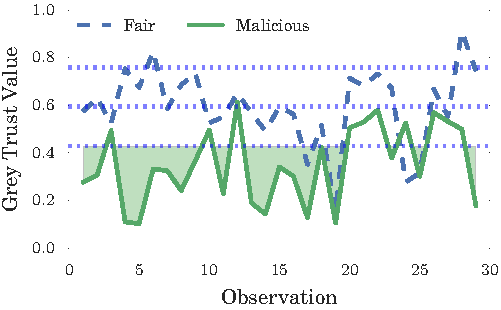
\includegraphics[width=.45\linewidth]{trust_bella_all_mobile_emph_PLR_BadMouthingPowerControl}
		\label{fig:all_mobile_badmouthing_plr}
		\caption{PLR Emphasised}
	\end{subfigure}
	
	\begin{subfigure}{0.5\textwidth}
		\caption{RX Power Emphasised}
		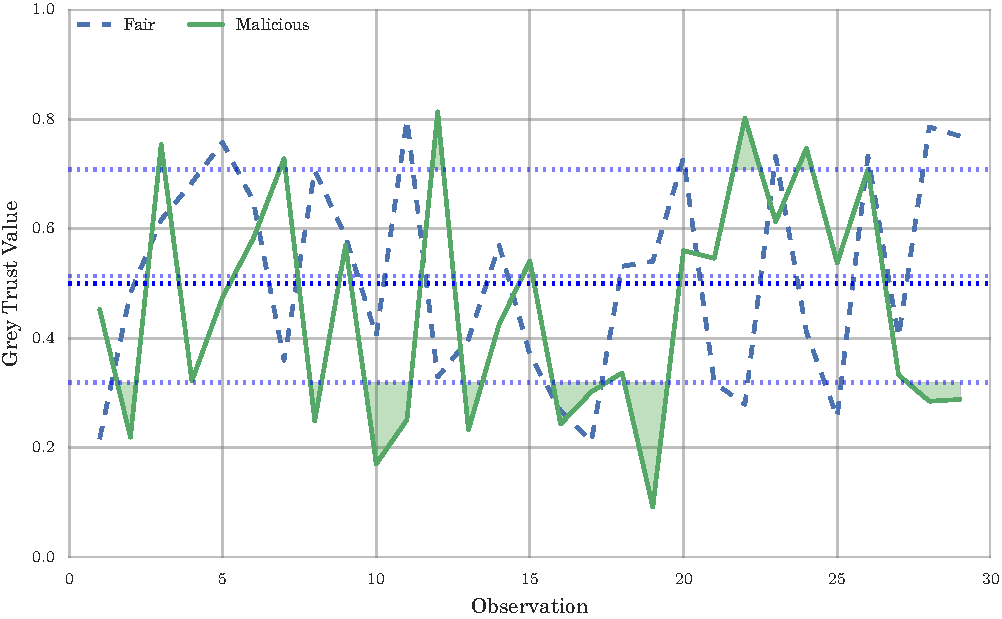
\includegraphics[width=.45\linewidth]{trust_bella_all_mobile_emph_ARXP_BadMouthingPowerControl} 
		\label{fig:all_mobile_badmouthing_rxp}
		\caption{TX Power Emphasised}
	\end{subfigure}	
	\begin{subfigure}{0.5\textwidth}
		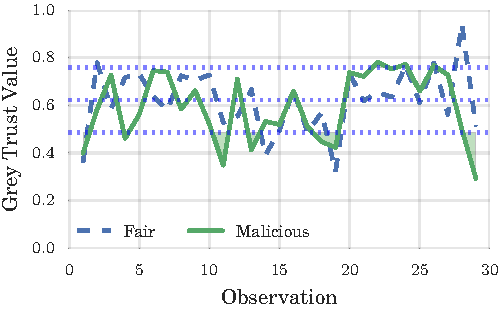
\includegraphics[width=.45\linewidth]{trust_bella_all_mobile_emph_ATXP_BadMouthingPowerControl}
		\label{fig:all_mobile_badmouthing_txp}
	\end{subfigure}
	
	\begin{subfigure}{0.5\textwidth}
		\caption{RX Throughput Emphasised}
		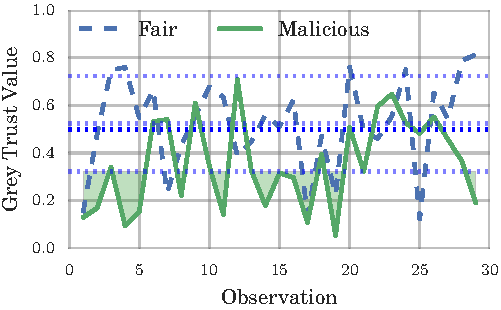
\includegraphics[width=.45\linewidth]{trust_bella_all_mobile_emph_RXThroughput_BadMouthingPowerControl} \label{fig:all_mobile_badmouthing_rxthroughput}
	\end{subfigure}
	\begin{subfigure}{0.5\textwidth}
		\caption{TX Throughput Emphasised}
		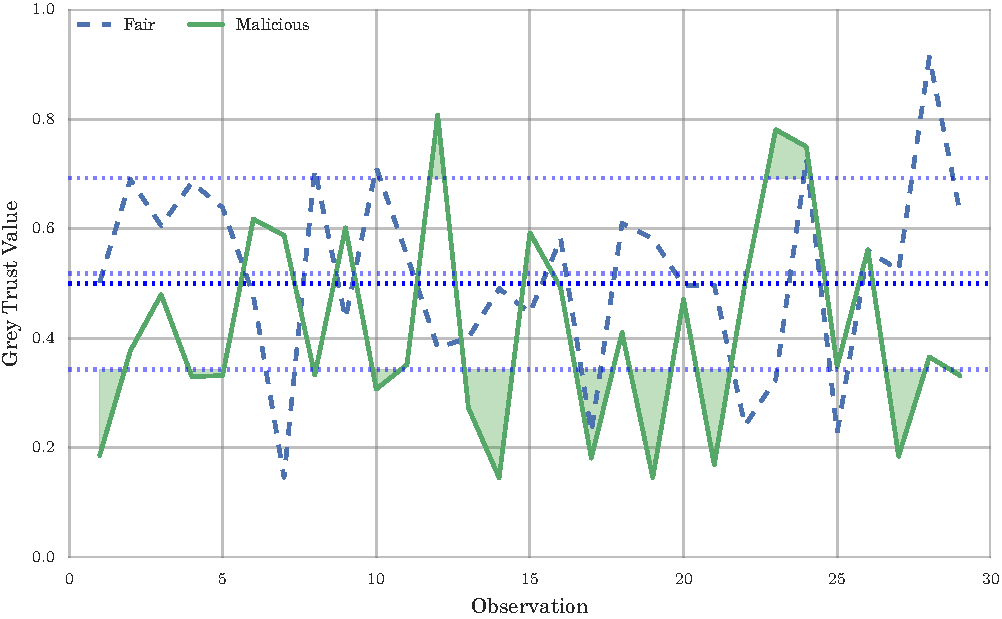
\includegraphics[width=.45\linewidth]{trust_bella_all_mobile_emph_TXThroughput_BadMouthingPowerControl} \label{fig:all_mobile_badmouthing_txthroughput}
	\end{subfigure}
	\caption{$T_{1,MTFM}$ in the All Mobile case for the Malicious Power Control behaviour, including dashed $\pm\sigma$ envelope about the fair scenario}
	\label{fig:all_mobile_badmouthing}
\end{figure}
%
\begin{figure}[h]
	\centering
	\begin{subfigure}{0.45\textwidth}	
	\caption{Delay Emphasised}
	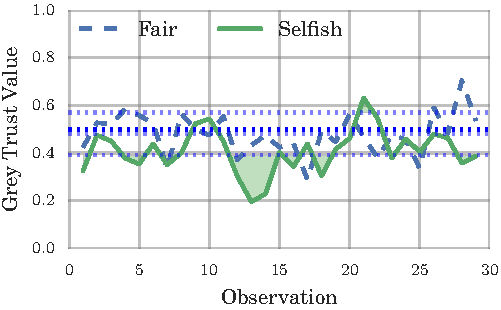
\includegraphics[width=\linewidth]{trust_bella_all_mobile_emph_ADelay_SelfishTargetSelection} 
	\label{fig:all_mobile_selfish_delay}
	\end{subfigure}
	\begin{subfigure}{0.45\textwidth}	
	\caption{PLR Emphasised}
	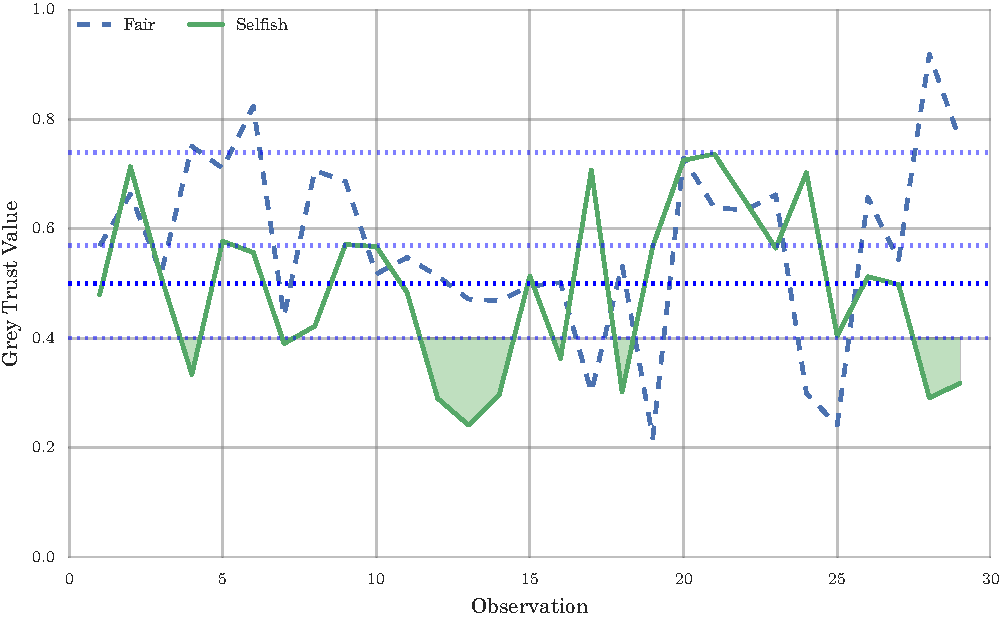
\includegraphics[width=\linewidth]{trust_bella_all_mobile_emph_PLR_SelfishTargetSelection}
	\label{fig:all_mobile_selfish_plr}
	
	\end{subfigure}
	\begin{subfigure}{0.45\textwidth}	
	\caption{RX Power Emphasised}
	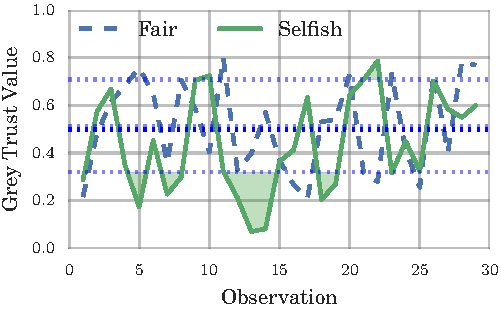
\includegraphics[width=\linewidth]{trust_bella_all_mobile_emph_ARXP_SelfishTargetSelection}
	\label{fig:all_mobile_selfish_rxp}
	\end{subfigure}
	\begin{subfigure}{0.45\textwidth}
	\caption{TX Power Emphasised}
	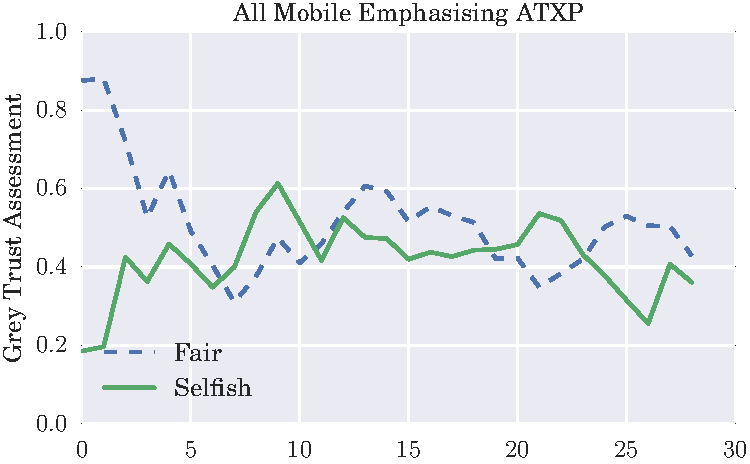
\includegraphics[width=\linewidth]{trust_bella_all_mobile_emph_ATXP_SelfishTargetSelection}
	\label{fig:all_mobile_selfish_txp}
	\end{subfigure}
	
	\begin{subfigure}{0.45\textwidth}
	\caption{RX Throughput Emphasised}
	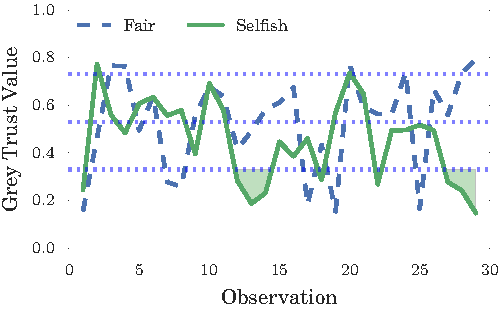
\includegraphics[width=\linewidth]{trust_bella_all_mobile_emph_RXThroughput_SelfishTargetSelection} 
	\label{fig:all_mobile_selfish_rxthroughput}
	\end{subfigure}
	\begin{subfigure}{0.45\textwidth}
	\caption{TX Throughput Emphasised}
	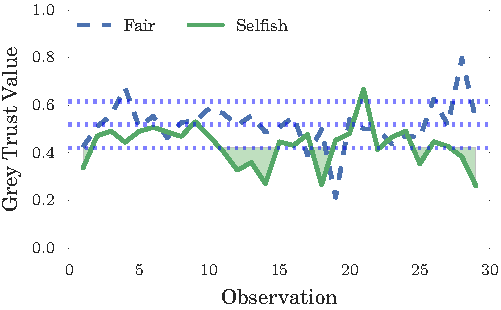
\includegraphics[width=\linewidth]{trust_bella_all_mobile_emph_TXThroughput_SelfishTargetSelection} \label{fig:all_mobile_selfish_txthroughput}
	\end{subfigure}
	\caption{$T_{1,MTFM}$ in the All Mobile case for the Selfish Target Selection behaviour, including dashed $\pm\sigma$ envelope about the fair scenario}
	\label{fig:all_mobile_selfish}
\end{figure}

From Fig.~\ref{fig:all_mobile_badmouthing} we can see that the malicious node is consistently outside the $\pm\sigma$ (one standard deviation above and below the mean) envelope of the fair scenario it's being compared to.
This is particularly true for PLR, with smaller impacts on delay, received power and transmitted throughput. 
This weighted delta in received throughput is minimal to insignificant compared to the width of the detection envelope, occasionally breaching the envelope for a short period. 

In the selfish case (Fig.~\ref{fig:all_mobile_selfish}) we observe much lower weighted delta in PLR and delay, with greatly increased impact on transmission power.
In comparison to \cite{Guo11}, these results are qualitatively similar, however here the differences between the fair case and the misbehaviours are less clear than in the comparable terrestrial space.
Guo et al. show similar types of behaviour but report a weighted delta from $\approx$ 0.4 to $\approx$ 0.9 across the simulation period, compared to our maximum delta in TX Power of $\approx$ 0.3 for an inconsistent interval (Fig.~\ref{fig:all_mobile_selfish_txp}.)


\subsection{Weight Significance Analysis for Behaviour Classification}

For a more quantitative assessment of the viability of multi-metric trust assessment methods, we take the qualitative analysis above and apply a Random Forest regression \cite{Breiman2001} to assess the relative importance of the selected metrics on relative detectability of malicious behaviour. 
Random Forest accomplishes this by generating a large number of random regression trees and prune these trees to fit incoming data.
The target function for this regression was the area between the target behaviours weighted $T_{MTFM}$ curve and the $\pm\sigma$ envelope of the base behaviour as shaded in Figs.~\ref{fig:all_mobile_badmouthing} and ~\ref{fig:all_mobile_selfish}.
From this training process we can extract the relative importance of each input feature (metric) in terms of how good it is to differentiate between the fair case and a given misbehaviour.
Additionally we perform a cross correlation analysis to establish the correlations between given metric weighting emphasis and the output of the target function.
Our intention is to establish the metrics that not only differentiate both misbehaviours from the fair case, but also what metrics differentiate the two misbehaviours from each other.

Applying this target regression to 729 different metric weight vector emphasis combinations reveals that each of the three combinations (i.e. comparing fair to misbehaviours, and comparing the misbehaviours) present distinct patterns of significance in three primary metrics; received throughput, transmitted power, and PLR, with delay, received power and transmitted throughput playing a lesser role.
Practically this means that in order to accurately distinguish between these scenarios, these primary metrics should be higher-weighted in the generation of $T_{1,MTFM}$ in \eqref{eq:networkeffects}.

It may initially appear odd that the relative significance of the received throughput is similar between all three scenario combinations, however a correlation analysis shows that in the MPC attack; the received throughput is positively correlated with successful classification against the fair case ($R=+0.71, p\approx10^{-100}$), while the inverse is the case for the STS attack ($R=-0.70, p\approx10^{-100}$).
It is expected that Transmitted power should be the defining characteristic of STS ($R=+0.72, p<10^{-100}$) as the node is acting fairly from a protocol perspective but is acting unfairly at a higher (incentive) level; it is performing fairly in terms of it's communications with other nodes, however it is preferring to communicate with nodes that it can expend less energy communicating with.
A summary of these correlations is shown in Table.~\ref{tab:correlations}.

Comparing Figs.~\ref{fig:otmf_beta_comparison},~\ref{fig:all_mobile_badmouthing_plr}, and ~\ref{fig:all_mobile_selfish_plr}, while it is possible that in a cleaner, less sparse, and less noisy environment, OTMF would be able to detect the MPC behaviour, from Fig.~\ref{fig:malselfactors} we see that PLR plays almost no part at all in detecting the STS behaviour, and so OTMF would not detect the attack.

\begin{figure}
	\centering
	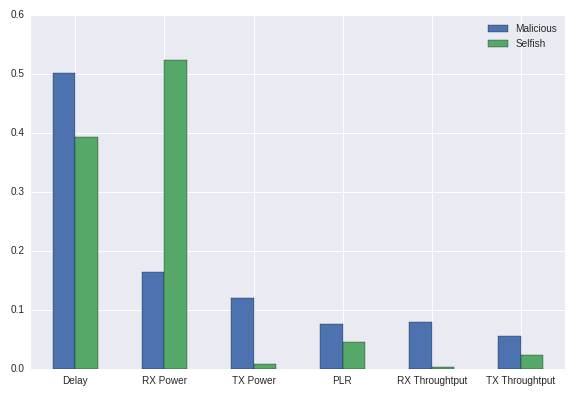
\includegraphics[width=0.95\linewidth]{MaliciousSelfishMetricFactors}
	\caption{Random Forest Factor Analysis of Malicious (MPC), Selfish (STS) and Fair behaviours compared against eachother}
	\label{fig:malselfactors}
\end{figure}

\begin{table}[h]
	\caption{Correlation Coefficients between metric weights and behaviour detection targets} \label{tab:correlations}
	\begin{center}
		\begin{tabular}{lcccccc}
			\toprule
			Correlation      & Delay & $P_{RX}$ & $P_{TX}$ & $T^P_{RX}$ & $T^P_{TX}$ & PLR \\
			\midrule
			Fair / MPC       & 0.199 &  0.159   & -0.416  &  0.708   & -0.238   & -0.401\\
			Fair / STS       & 0.179 &  -0.009  &  0.724  & -0.697   & -0.145   & -0.052\\
			MPC / STS        & 0.058 &  -0.134  &  0.146  & -0.768   &  0.052   &  0.146\\
			\bottomrule
		\end{tabular}
	\end{center}
\end{table}

As such this presents the open opportunity to develop a heuristic weight search scheme to detect malicious behaviour without the comparison to the fair scenario.
This would be accomplished by assessing the impact of differential metric weighting on the mean trust assessment rather than comparing co-weighted valuations across scenarios.


\section{Conclusions and Future Work}
We have demonstrated that existing MANET Trust Management Frameworks are not directly suitable to the sparse, noisy, and dynamic underwater medium.
We presented a comparison between trust establishment in MANETs in a simulated underwater environment, demonstrating that in order to have any reasonable expectation of performance, throughput and delay responses must be characterised before implementing trust in such environments. 
While the MTFM value does not display any immediate difference between the two behaviours, we have shown that by exploring the metric space by weight variation, the existence and nature of the malicious behaviour can be discovered.
Another difference is that MTFM is significantly more computationally intensive than the relatively simple Hermes / OTMF algorthms.
The repeated metric re-weighting required for real time behaviour detection is therefore an area that requires optimization.
We demonstrated initial, unfiltered Grey Trust assessment using all available metrics (transmitted and received throughput, delay, received signal strength, transmitted power, and packet loss rate), as well as the application of multiple weighting vectors to iteratively emphasise different aspects of trust operation to expose and identify misbehaviour on the network.
With significant delays (from seconds to many minutes), in a fading, refractive medium with varying propagation characteristics, the environment is not as predictable or performant as classical MANET TMF deployment environments.

We show that, without significant adaptation, single metric probabilistic estimation based TMFs are ineffective in such an environment.
We have shown that existing frameworks are overly optimistic about the nature and stability of the communications channel, and can overlook characteristics that are useful for assessing the behaviour of nodes in the network. 
This indicates that there is a good case, particularly within constrained MANETs as this, for multi-vector, and even multi-domain trust assessment, where metrics about the communications network and topology would be brought together with information about the physical behaviours and operations of nodes to assess trust.

Also, a significant factor of trust assessment in such a constrained environment, is that there may be long periods where two edge nodes (for instance, $n_0 \to n_5$) may not interact at all. 
This can be due to a range of factors beyond malicious behaviour, including simple random scheduling coincidence and intermediate or neighbouring nodes collectively causing long back-off or contention periods.
This disconnection hinders trust assessment in two ways; assessing nodes that do not receive timely recommendations may make decisions based on very old data, and malicious nodes have a long dwelling time where they can operate under a reasonable certainty that the TMF will not detect it (especially if the node itself is behaving disruptively).
One solution to this would be to move from a stepping-window of trust observations to a continuous trust log, updated on packet reception rather than waiting regular periods for packets to be analysed.
Future work will investigate the improvement of weight-based detection algorithms, the stability of GRA under multi-node collusion, the development of real-time outlier detection, and the introduction of physical behavioural metrics into the trust assessment context.



\subsection{Metric Weighting}
\begin{figure}
\begin{subfigure}{.5\textwidth}
  \centering
  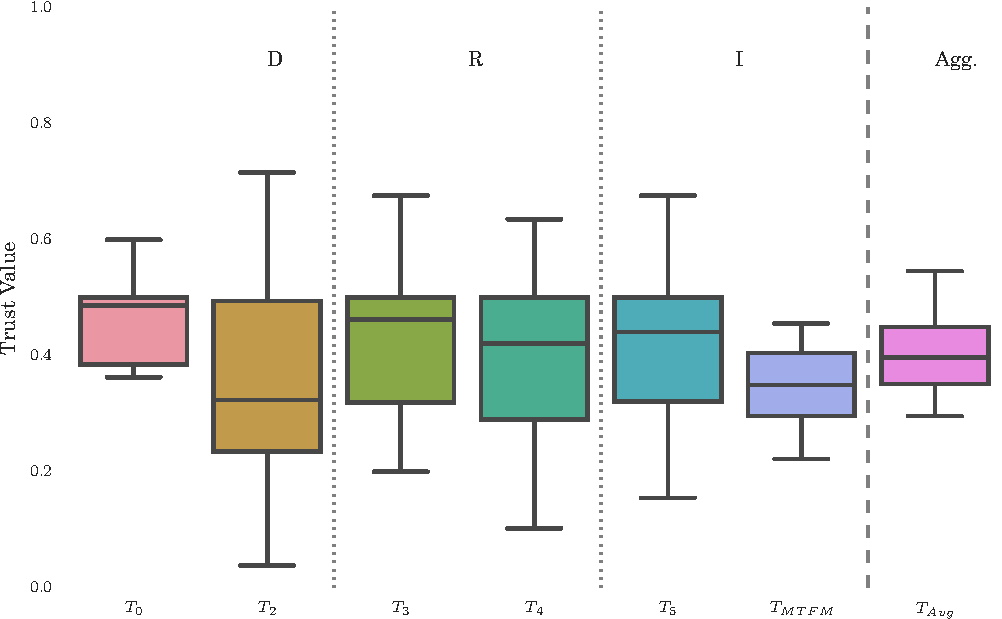
\includegraphics[width=.95\linewidth]{trust_bella_static_selfish.pdf}
  \caption{All Nodes Static}
  \label{fig:selfish_trust_static}
\end{subfigure}%
\begin{subfigure}{.5\textwidth}
  \centering
  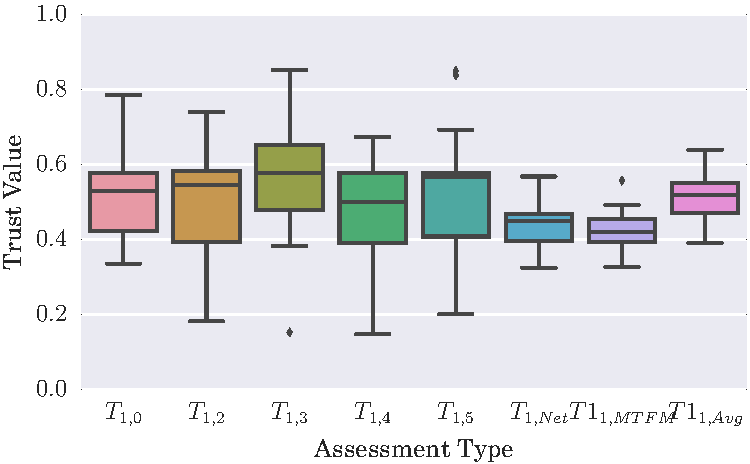
\includegraphics[width=.95\linewidth]{trust_bella_single_mobile_selfish.pdf}
  \caption{$n_1$ Randomly Walking}
  \label{fig:selfish_trust_single}
\end{subfigure}
\begin{subfigure}{.5\textwidth}
\centering
  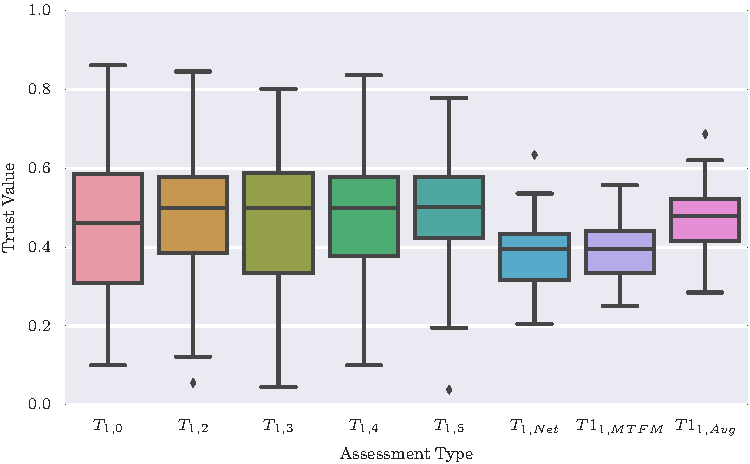
\includegraphics[width=.95\linewidth]{trust_bella_allbut1_mobile_selfish.pdf}
  \caption{All Nodes but $n_1$ Randomly Walking}
  \label{fig:selfish_trust_allbut1}
\end{subfigure}
\begin{subfigure}{.5\textwidth}
\centering
  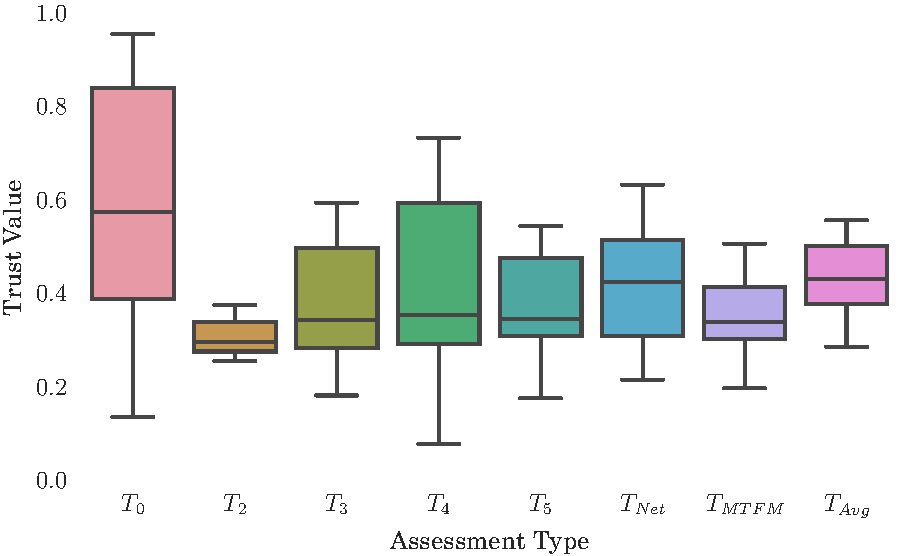
\includegraphics[width=.95\linewidth]{trust_bella_all_mobile_selfish.pdf}
  \caption{All Nodes Randomly Walking}
  \label{fig:selfish_trust_all_mobile}
\end{subfigure}
\caption{MTFM Trust assessments for varying mobility options in the selfish case}
\label{fig:trust_mobility}
\end{figure}



\begin{figure}
\begin{subfigure}{0.5\textwidth}
  \centering
  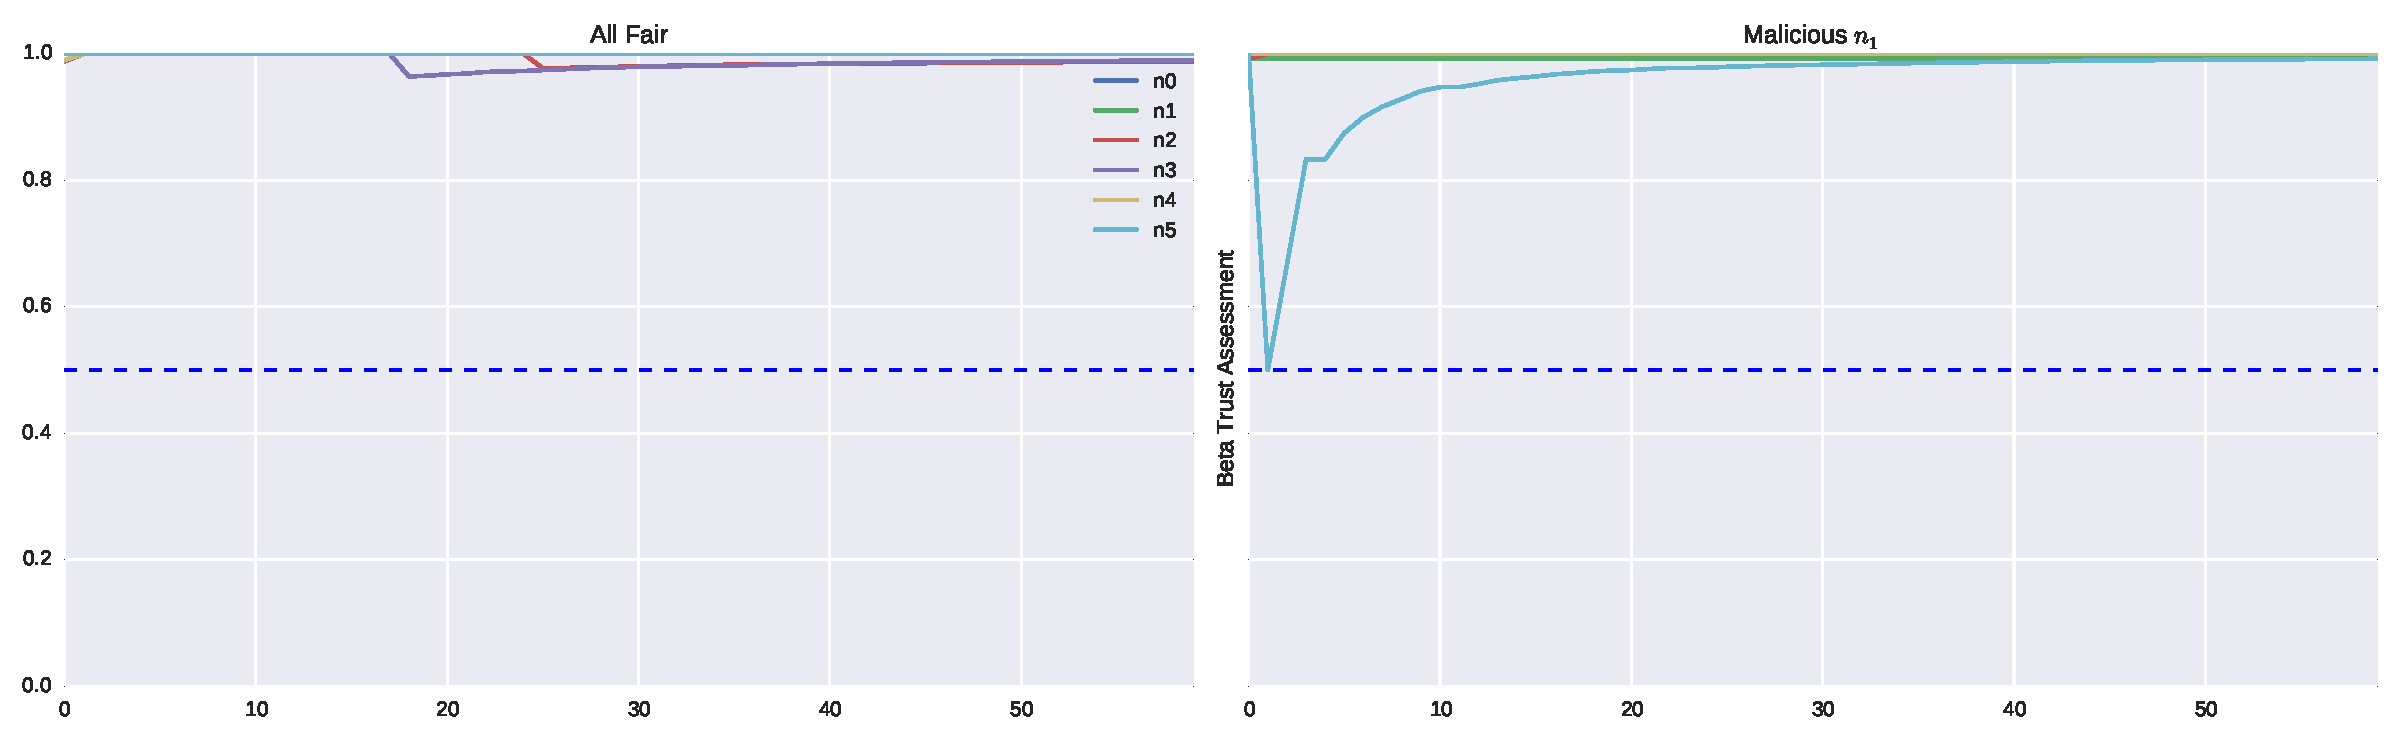
\includegraphics[width=.95\linewidth]{beta_trust_bella_static_joint.pdf}
  \caption{All Nodes Static}
  \label{fig:beta_trust_static}
\end{subfigure}%
\begin{subfigure}{0.5\textwidth}
  \centering
  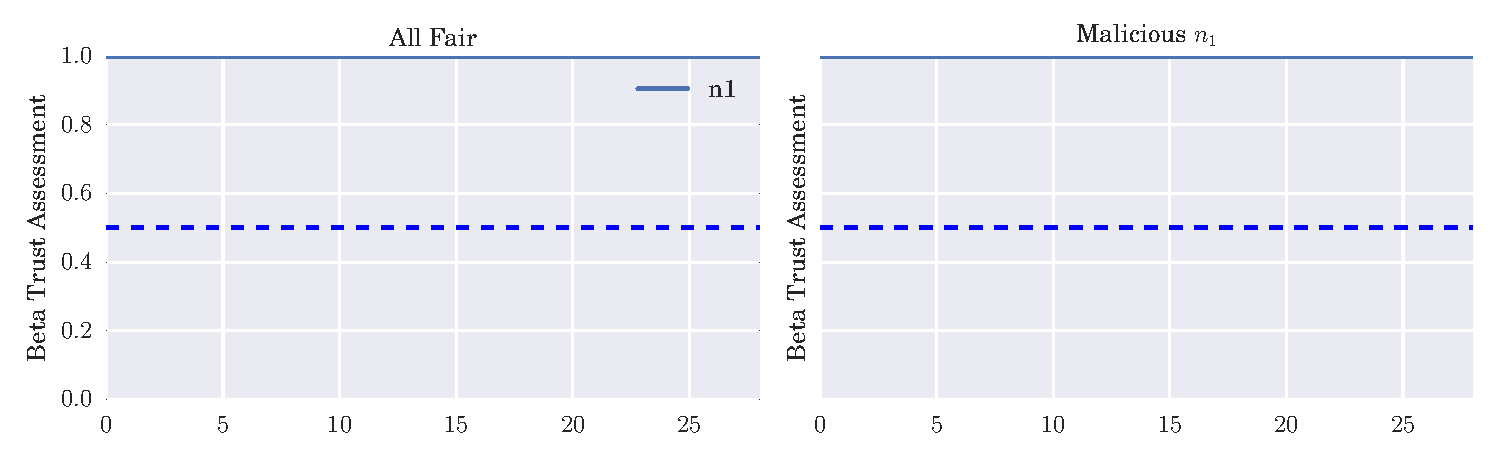
\includegraphics[width=.95\linewidth]{beta_trust_bella_single_mobile_joint.pdf}
  \caption{$n_1$ Randomly Walking}
  \label{fig:beta_trust_single}
\end{subfigure}%

\begin{subfigure}{0.5\textwidth}
\centering
  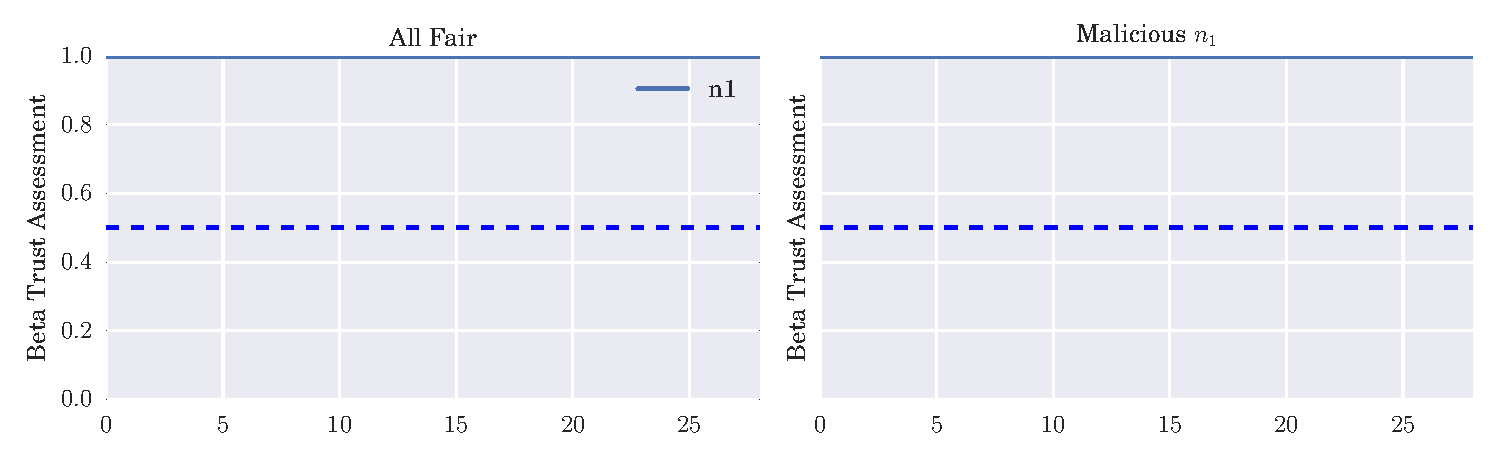
\includegraphics[width=.95\linewidth]{beta_trust_bella_allbut1_mobile_joint.pdf}
  \caption{All Nodes but $n_1$ Randomly Walking}
  \label{fig:beta_trust_allbut1}
\end{subfigure}%
\begin{subfigure}{0.5\textwidth}
\centering
  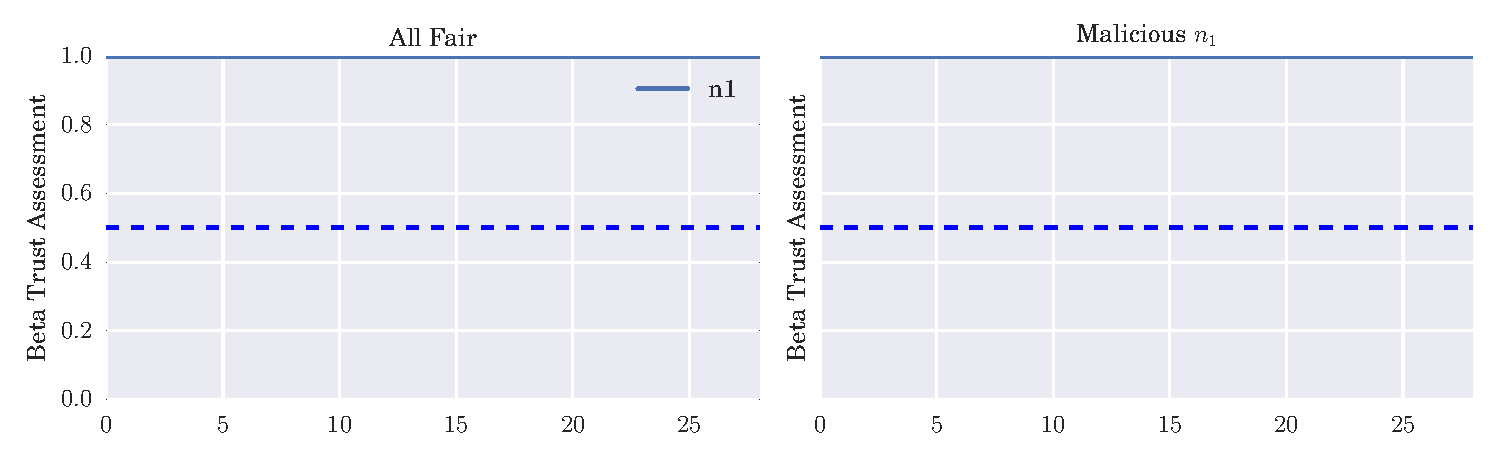
\includegraphics[width=.95\linewidth]{beta_trust_bella_all_mobile_joint.pdf}
  \caption{All Nodes Randomly Walking}
  \label{fig:beta_trust_all_mobile}
\end{subfigure}
\caption{Beta Trust time varying assessments for of $n1$ varying mobility options}
\label{fig:trust_mobility}
\end{figure}



 % Modelling and Analysis of Collaborative Node Kinematic Behaviuors in Underwater Acoustic MANETs

% !TeX spellcheck = en_GB
\def\ChapterTitle{Multi-Domain Trust Assessment in Collaborative Marine \gls{manet}s}

\chapter{\ChapterTitle}
\label{Chapter\thechapter}
\lhead{Chapter \thechapter. \emph{Analysis of Multi-Domain Trust Assessment}} % Write in your own chapter title to set the page header

\section{Introduction}

In this chapter, a multi-domain trust management framework (MD-TMF) is demonstrated in collaborative marine \glspl{manet}
A methodology is demonstrated that applies Grey Sequence operations and Grey Generators to provide continuous trust assessment in a sparse, asynchronous metric space across multiple domains of trust.
By utilising information from multiple domains, it is demonstrated that trust assessment can be more accurate and consistent in identifying misbehaviour than in single-domain assessment.
Further, a methodology for assessing the usefulness of individual metrics in this cross-domain space is demonstrates, allowing for the elimination of redundant metrics, simplifying the runtime assessment process.

\section{Construction of Multi-Domain Trust}

A key question in this chapter is to assess the advantages and disadvantages of utilising trust from across domains. 
This includes a secondary question as to how trust assessments from these domains are most effectively combined. 

It is important to clarify what is meant by ``effective'' in this case; the ``effectiveness'' of any trust assessment framework is taken as consisting of several parts.

\begin{enumerate}
  \item the \emph{accuracy} of detection and identification of a particular misbehaviour
  \item the \emph{timeliness} of such detections
  \item the \emph{complexity} of such analysis, including any specific training required
  \item the \emph{commonality} of the results of any detections between perspectives (also termed ``isomorphism'' of results)
\end{enumerate}



\subsection{Communications Trust Metrics}

The metric vector is constructed using those trust metrics that are applicable to the marine environment from \cite{Guo2012}, as the simulated marine acounstic modem stack does not operate on the same tiered data-rate approach as used in the 802.11 stack, the data rate metric was not included. Remaining metrics are; Delay, Received and Transmitted power, Received and Transmitted Throughput, and \gls{plr}.

Thus, the metric vector used for communications-trust assessment is;

\begin{equation}
	X_{comms}=\{D, P_{RX}, P_{TX}, Tp_{RX}, Tp_{TX}, PLR\}
	\label{eq:comms_vector}
\end{equation}

\subsection{Physical Trust Metrics}

Three physical metrics are selected to encompass the relative distributions and activities of nodes within the network; \gls{indd}, \gls{inhd}, and Node Speed. These metrics encapsulate the relative distributions of position and velocity within the fleet, optimising for the detection of outlying or deviant behaviour within the fleet.

Conceptually, \gls{indd} is a measure of the average spacing of an observed node with respect to its neighbours. \gls{inhd} is a similar approach with respect to node orientation.

\begin{align}
	INDD_{i,j} &= \frac{|P_j - \sum_x \frac{P_x}{N}|}{\frac{1}{N}\sum_x \sum_y{|P_x - P_y| (\forall x \neq y)}}\\
	INHD_{i,j} &= \hat{v} \vert v= V_j - \sum_x{\frac{V_x}{N}}\\
	S_{i,j} &= |V_j|
\end{align}

Thus, the metric vector used for physical-trust assessment is;

\begin{equation}
  X_{phy}=\{\text{INDD}, \text{INHD}, S\}
	\label{eq:phys:vector}
\end{equation}
\todo{Need to actually show physical only trust measurements}

\subsection{Cross Domain Trust Metrics}
This simplest possible combination is a vector concatenation across domain metric vectors; in this case; 

\begin{equation}
  X_{merge} =  (X_{comms}|X_{phy}) = \{D, P_{RX}, P_{TX}, Tp_{RX}, Tp_{TX}, PLR, \text{INDD}, \text{INHD}, S\}
	\label{eq:phys:vector}
\end{equation}


\subsection{Metric Weight Analysis Scheme}

From \eqref{eq:metric_weighting}, the final trust values arrived at are dependent on metric values, the weights assigned to each metric, and the structure of the $g$, $b$ comparison vectors.\todo{referencing the right equ in the wrong place}

This permits the assessment of the significance of different metrics in the detection and identification of different behaviours. 
The primary aspects of an (mis)behaviour can be detected and assessed by comparing a weighted trust assessment against the deviation from a ``fair'' result set using the same weight, i.e.\ we are interested in the weight schemes that create the largest difference between fair and misbehaving cases.\todo{Possibly redundant sentences}

For a metric weight vector $H$, where the metric $m_j$ is emphasised as being twice as important as the other metrics, an initial weighting vector $H'=[h_i\cdots h_M]$ is formed such that $h_i = 1 \forall i \ne j; h_j=2$. That vector $H'$ is then scaled such that $\sum H = 1$ by $H= \frac{H'}{\sum H'}$.

The construction of the $g$ and $b$ vectors from~\autoref{eq:grc} depends on the particular metric, e.g. Throughput ($T^P$) on a link is assumed to be positively correlated to trustworthiness and so follows the default construction ($g(T^P) \mapsto \max, b(T^P) \mapsto \min$), whereas in the case of a metric such as delay, this relationship is inverted, i.e.\ longer delays indicate less trustworthy activity ($g(D) \mapsto \min, b(D) \mapsto \max$).
This inversion relationship (i.e.\ those with the construction $g(x) \mapsto \min, b(x) \mapsto \max$) is signified by a negative weight.

In complex environments, the relationship between metrics trustworthiness correlations is not always as obvious as the throughput / delay examples.
This phenomenon was mentioned by Guo\cite{Guo2012}, but was manually configured for each metric for each behaviour and no analytical method for quantitatively establishing such relationships has been presented since.

With the nine selected metrics from across communications and physical behaviours, we can explore this metric space by varying the weights associated with each metric, and choose to emphasise across three levels; i.e.\ metrics can be ignored or over-emphasised. Naively this results in $3^9 = 19683$ combinations, however as these weights are being normalised, redundant duplicates can be eliminated, e.g. $[0,0,0,0,1,0,0,0,0] \equiv [0,0,0,0,2,0,0,0,0]$ leaving 18661 unique weights for analysis.

To assess the performance of a given weight combination (i.e.\ an optimisation factor), we are initially interested in the metric weight vector that consistently provides the largest deviation in the final trust value $T$ across the cohort, i.e.\ producing the most clear detection of a node misbehaving in that particular fashion.
This is approached as an inverse outlier filtering problem, and the range outside a $\pm\sigma$ envelope compared to the equivalent weighting in a known ``fair'' behaviour is selected to assess detection (or comparing to other misbehaviours to assess discrimination).
See~\autoref{sec:metric_weighting}.
Note that at this point we establish ``signatures'' of different behaviours rather than optimal detection weights.\todo{Duplicating C6 Metric Weighting Section}

We apply a Random Forest regression \cite{Breiman2001} to assess the relative importance of the selected metrics on relative detectability of malicious behaviour. 
Random Forest accomplishes this by generating a large number of random regression trees and prune these trees to fit incoming data. A major advantage of Random Forest in this case is that by walking the most successful regression trees, we can acquire an already normalised maximal activation weight for the particular behaviour comparison being tested.

After establishing the importance of weights in particular behaviours, a final weight is arrived at by algorithmically those few metrics that are important, rather than having to further explore the computationally expensive weight-space.

Using this approach, the results of these simulations can be explored, condensing the multi-dimensional problem (target / observer / behaviour / metric / time) down to a more manageable level for analysis.

\section{Results and Discussion}

\subsection{Significance Analysis}

First the results of the Random Forest regression assessment are discussed; Figs~\ref{fig:comms_feature_extraction} and~\ref{fig:phys_feature_extraction}, show the resultant feature extraction signatures for Comms-only and Physical-only metric selections respectively, and in Fig~\ref{fig:multi_feature_extraction}, these metric spaces are brought together and reassessed.

In both single-domain cases, there are clear ``signatures'' in misbehaviours that don't directly target that domain ($P_{RX}$ in the Physical Shadow and Slowcoach behaviours in Fig~\ref{fig:comms_feature_extraction} and $INDD$ in the Selfish Target Selection behaviour in Fig~\ref{fig:phys_feature_extraction}).
This inter-domain activity is to be expected in \glspl{manet} in general, where the physical reality of the network (i.e.\ distance between nodes) directly impacts the behaviour of the logical communications network (i.e.\ delay between nodes), and is a useful characteristic for differentiating potential misbehaviours.\todo{Come back to this and talk about redundancy}



\begin{figure}[h!]
	\centering
  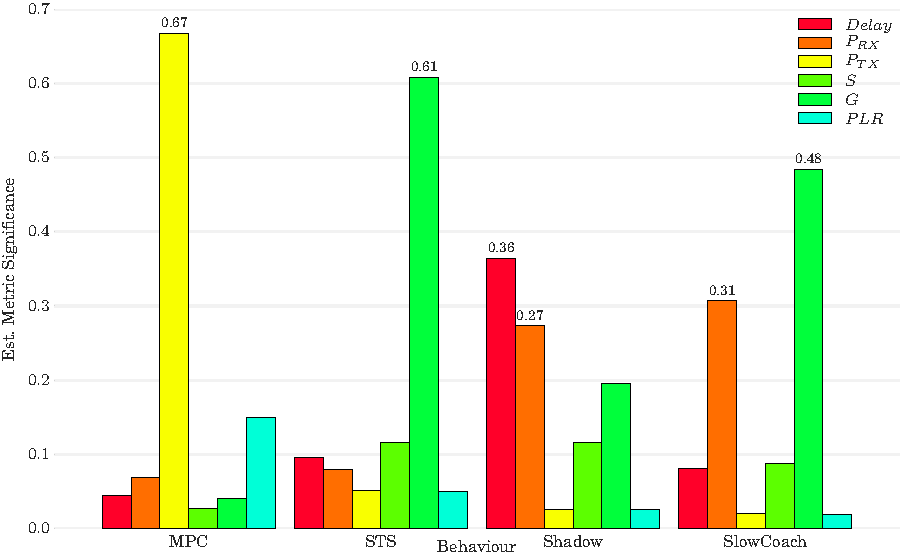
\includegraphics[width=\linewidth]{comms_metric_trust_relevance}
	\caption{Plot of Communications Metric Feature Extraction ($X_{comms}$)}
	\label{fig:comms_feature_extraction}
\end{figure}

\begin{figure}[h!]
	\centering
  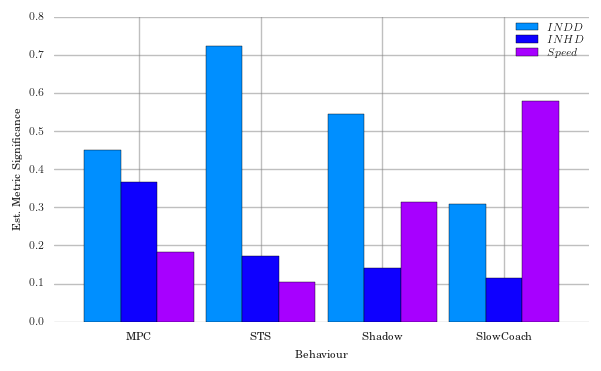
\includegraphics[width=\linewidth]{phys_metric_trust_relevance}
  \caption{Plot of Physical Metric Feature Extraction ($X_{phys}$)}
	\label{fig:phys_feature_extraction}
\end{figure}

\begin{figure}[h!]
  \centering
  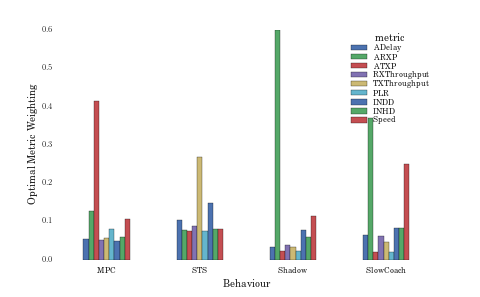
\includegraphics[width=\linewidth]{full_metric_trust_relevance}
  \caption{Multi Domain  Metric Features Extraction $X_{merge}$}
  \label{fig:multi_feature_extraction}
\end{figure}

%\begin{tabular}{lrrrrrrrrr}
\toprule
{} &  $Delay$ &  $P_{RX}$ &  $P_{TX}$ &  $T^P_{RX}$ &  $PLR$ &  $T^P_{TX}$ &  $INDD$ &  $INHD$ &  $Speed$ \\
Misbehaviour &          &           &           &             &        &             &         &         &          \\
\midrule
MPC          &   -0.187 &     0.129 &     0.579 &       0.006 &  0.069 &      -0.146 &   0.040 &  -0.190 &   -0.297 \\
STS          &   -0.195 &    -0.035 &     0.019 &      -0.100 &  0.019 &       0.381 &  -0.209 &   0.057 &    0.062 \\
Shadow       &    0.004 &    -0.654 &     0.030 &      -0.016 &  0.030 &       0.063 &   0.120 &   0.158 &    0.266 \\
SlowCoach    &   -0.157 &    -0.533 &     0.013 &      -0.132 &  0.013 &      -0.028 &   0.159 &   0.206 &    0.460 \\
\bottomrule
\end{tabular}


\subsection{Weight Assessment}

From this significance information, a ``estimated'' signature for each behaviour can be inferred, which can then be fed back into the assessment framework. 
The aim of this iteration is to minimise the number of weight permutations required to come to a conclusion about the behaviour under observation. 

However, these approximated signatures have no information regarding the ``sign'' of the  $g$,$b$ comparison vectors from \eqref{eq:metric_weighting}, i.e.\ there is no hint as to whether the relationship is $g(x) \mapsto \max, b(x) \mapsto \min$ or $g(x) \mapsto \min, b(x) \mapsto \max$)  

One option would be to go back to the regression point and expand the combination options to include negative values, signifying inverted $g,b$ relationships, however this is combinatorially explosive.\footnote{The current version of this analysis uses three metric weights; ignored, standard, emphasised, giving $3^9 = 19683$ combinations. Expanding this to include inverted standard and inverted emphasised weights would raise that to $5^9 = 1.9\times 10^6$}
Instead, the ``significance'' weight is permuted against it's possible combinations of ``flips'', i.e.\ for $X_s=[0.3,0.4,0.01,0.02,0.27]$ could also be $X_s^p=[0.3,-0.4,0.01,0.02,0.27]$ and so on. 
This sign permutation is filtered based on a threshold value ($0.01$), so for all indices below that threshold will not be permuted on, halving the number of combinations required for each indices eliminated.
This reduces the number of additional assessments required from $1.9$ to approximately 500 (when applied to all nine metrics).

The best of these permutations is selected to both maximise the (correct) deviation between each nodes trust perspectives and to minimise the trust value reported for the misbehaving nodes; $\Delta T \max$

These weights are applied to untrained simulation data to derive the following results.

An exemplar subset of the results is shows in Figs~\ref{fig:comms_sts}-~\ref{fig:full_slowcoach}, with the ``misbehaving node'' highlighted with heavier lines, with any observations about the rest of the cohort faded and dashed. For each node assessment, the mean for that assessment over that time period is also included as a solid / dashed line respectively for clarity.

Comparing Figs~\ref{fig:comms_sts} and~\ref{fig:full_sts}, while there is a reasonable dip in the misbehavor's trust assessment, the variance across the cohort is such that this "mistrust" triggering is neither consistent or obvious. Unfortunately this is the case across the \gls{sts} responses, where in Table~\ref{tab:domain_deltas} where we have summarized out general results, \gls{sts} has by far and away the lowest average $\Delta T$ in all domains. Interestingly however is the observation that Comms-only trust performs slightly better than Full trust weighting.

Referring to Figs~\ref{fig:comms_feature_extraction} and~\autoref{fig:multi_feature_extraction}, it's clear that the transmitted throughput ($T^P_{TX}$) is the almost singular feature of this behaviour, due to it's almost completely logical behaviour that is only loosely coupled to the state of the environment. 
The massive emphasis placed on throughput could only be diminished by putting it together in a larger ensemble.

The other "Primary Communications" behaviour, \gls{mpc}, is not shown for brevity, but scores comfortably in the 90th percentile range in both full and comms trust assessments.

In Figs~\ref{fig:comms_shadow} and~\ref{fig:full_shadow}, the misbehaving node is much more obvious than in \gls{sts}, which is moderately surprising for a physically-focused behaviour. Further, there is a roughly 20\% improvement when incorporating the full metric space.

From Table~\ref{tab:domain_deltas}, the Shadow behavior is the most consistently detectable behaviour across domains. 

\begin{figure}[h]
	\centering
	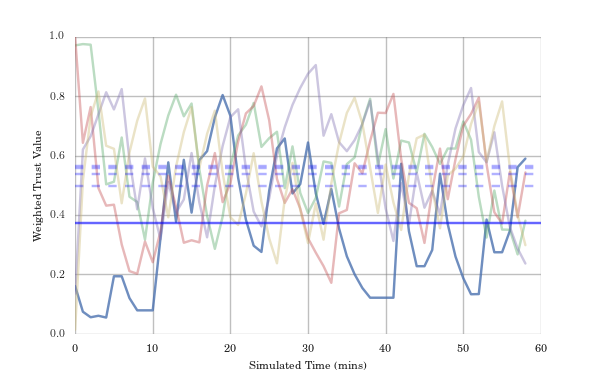
\includegraphics[width=\linewidth]{best_comms_run_STS}
	\caption{Selfish(STS) Targeting Comms Metric Trust}
	\label{fig:comms_sts}
\end{figure}

\begin{figure}[h]
	\centering
	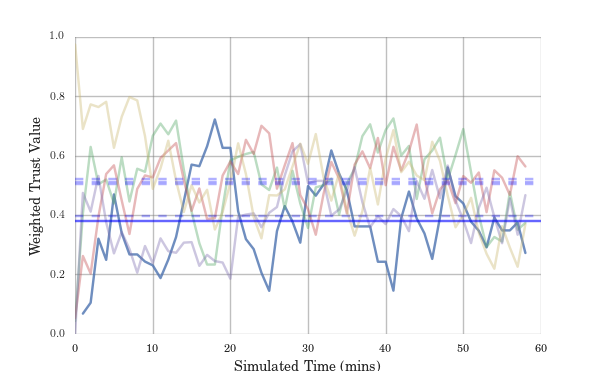
\includegraphics[width=\linewidth]{best_full_run_STS}
	\caption{Selfish(STS) Targeting Full Metric Trust}
	\label{fig:full_sts}
\end{figure}

\begin{figure}[h]
	\centering
	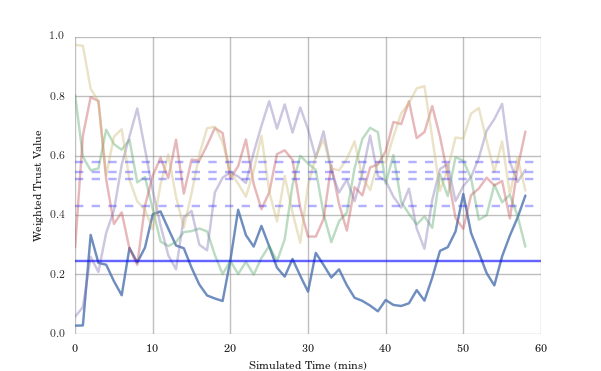
\includegraphics[width=\linewidth]{best_comms_run_Shadow}
	\caption{Shadow Comms Metric Trust}
	\label{fig:comms_shadow}
\end{figure}

\begin{figure}[h]
	\centering
	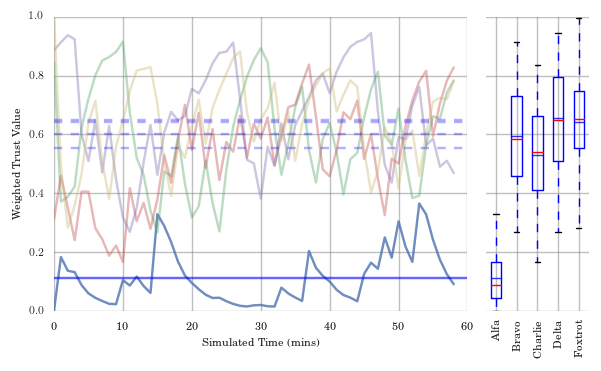
\includegraphics[width=\linewidth]{best_full_run_Shadow}
	\caption{Shadow Full Metric Trust}
	\label{fig:full_shadow}
\end{figure}


\begin{figure}[h]
	\centering
  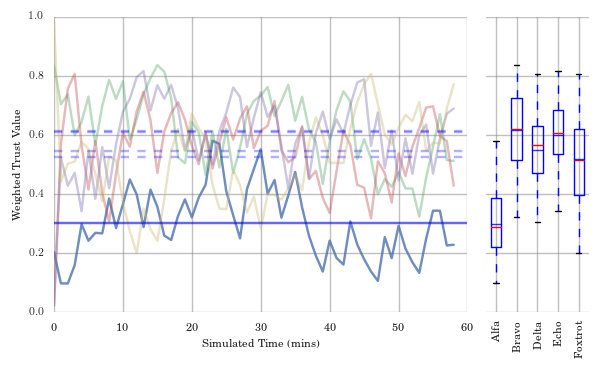
\includegraphics[width=\linewidth]{best_comms_run_SlowCoach}
	\caption{SlowCoach Comms Metric Trust}
	\label{fig:comms_slowcoach}
\end{figure}


\begin{figure}[h]
	\centering
  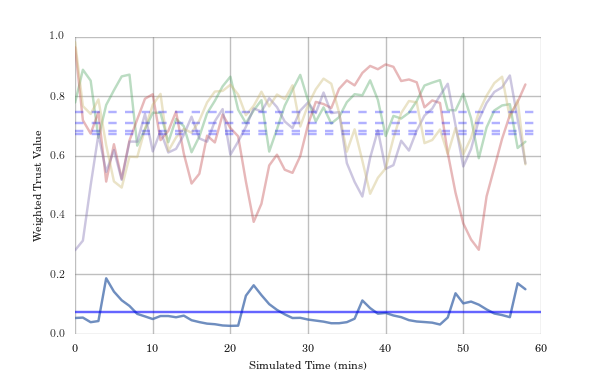
\includegraphics[width=\linewidth]{best_full_run_SlowCoach}
	\caption{SlowCoach Full Metric Trust}
	\label{fig:full_slowcoach}
\end{figure}


\begin{table}
\centering
\caption{$\Delta T$ across domains and detected behaviours}
\begin{tabular}{|l|r|r|r|r|r|}
\hline
\diagbox{Domain}{Behaviour} &       \gls{mpc} &       \gls{sts} &    Shadow & SlowCoach & Avg.\\
\hline
%Domain &           &           &           &           &\\
Comms  &  0.954 &  0.166 &  0.287 &  0.268 & 0.419 \\
Phys   &  0.022 &  0.020 &  0.421 &  0.756 & 0.305\\
Full   &  0.905 &  0.101 &  0.499 &  0.627 & 0.533\\
\hline
Avg.   &  0.627 &  0.096 &  0.402 &  0.550 &  0.419 \\
\hline
\end{tabular}
\label{tab:domain_deltas}
\end{table}

\section{Conclusion}
In this paper we demonstrate that in harsh environments, multi-domain trust assessment can perform better on average than single-domain counterparts, both in terms of robustness and sensitivity, but also covering a wider region of the potential behaviour space, 

The extension of the methodologies of multi-vector trust into the marine space are already demonstrated, however including information from physical observations of actors in a network enables the detection and identification of a much wider range of behaviours.
We also demonstrate a method for assessing trust metrics in harsh environments in terms of their relative significance, and a method for establishing classification signatures for misbehaviours.

It is to be noted that this presented method is significantly more computationally intensive than the relatively simple Hermes / OTMF algorithms communications only algorithms, and is exponential in complexity as metrics and/or domains are added. The repeated metric re-weighting required for real time behaviour detection is therefore an area that requires optimization. More work needs to be done to characterise how worthwhile this approach is compared to a separate synthesis approach where by MTFM-style trust is generated and assessed on a per-domain basis and subsequently fuzed.

For greater fidelity and more optimal results, a wider range of weights can be used in the initial regression step; however this is computationally expensive given that weighting is applied to each perspective (i.e.\ observer/target node pair) for each trust assessment time step, presenting 15 perspectives at each time interval in the 6 node case.

Every effort has been made to avoid over-training the dataset, using cross validating sampling for regression and "best weight" generation, however more meta-analysis is required to further demonstrate the functionality of this process.



%%%%%%%%%%%%%%%%%%%%%%%%%%%%%%%%%%%%%%%%%%%%%%%%%%%%%%%%%%%%%%%%%%%%%%%%%%%%%%%
 % Comparative Analysis of Multi-Comain Trust Assessment in Collaborative Module Networks



%% ----------------------------------------------------------------
% Now begin the Appendices, including them as separate files

\addtocontents{toc}{\vspace{2em}} % Add a gap in the Contents, for aesthetics

\appendix % Cue to tell LaTeX that the following 'chapters' are Appendices

% Appendix A

\chapter{Orphan Sections}
\label{AppendixA}
\lhead{Appendix A. \emph{Orphan Sections}}

\section{Metric Weighting}
\begin{figure}
\begin{subfigure}{.5\textwidth}
  \centering
  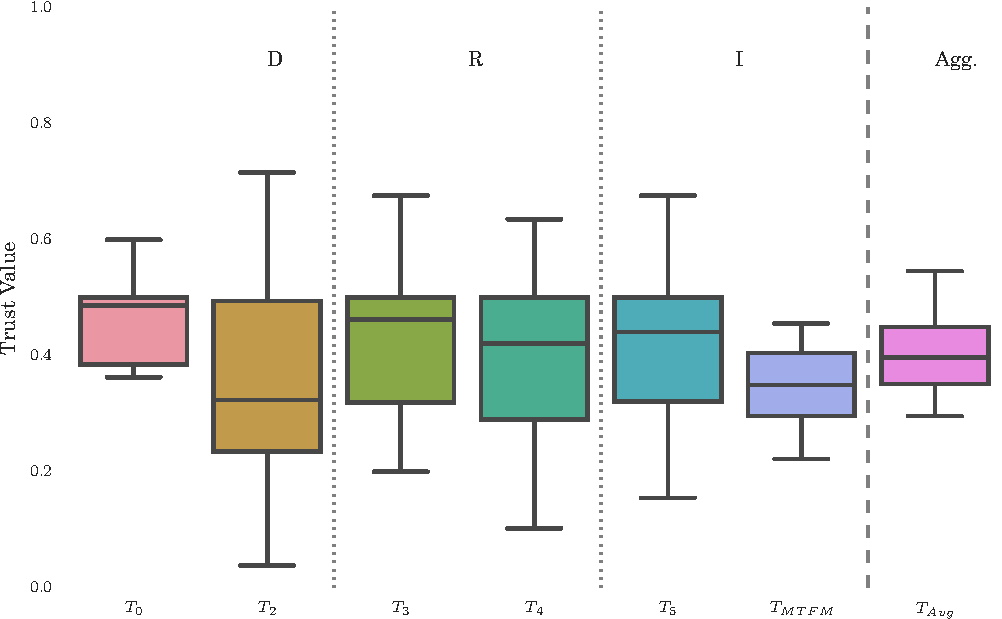
\includegraphics[width=.95\linewidth]{trust_bella_static_selfish}
  %\missingfigure[figwidth=.95\linewidth]{trust bella static selfish}
  \caption{All Nodes Static}
  \label{fig:selfish_trust_static}
\end{subfigure}%
\begin{subfigure}{.5\textwidth}
  \centering
  %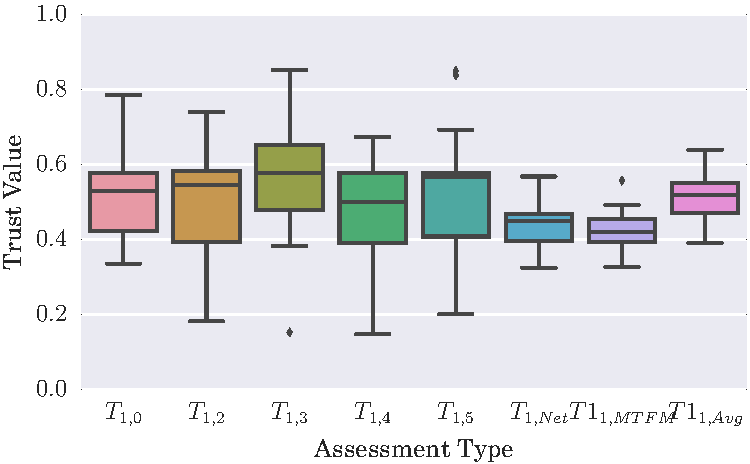
\includegraphics[width=.95\linewidth]{trust_bella_single_mobile_selfish}
  \missingfigure[figwidth=.95\linewidth]{trust bella single mobile selfish}
  \caption{$n_1$ Randomly Walking}
  \label{fig:selfish_trust_single}
\end{subfigure}
\begin{subfigure}{.5\textwidth}
\centering
  %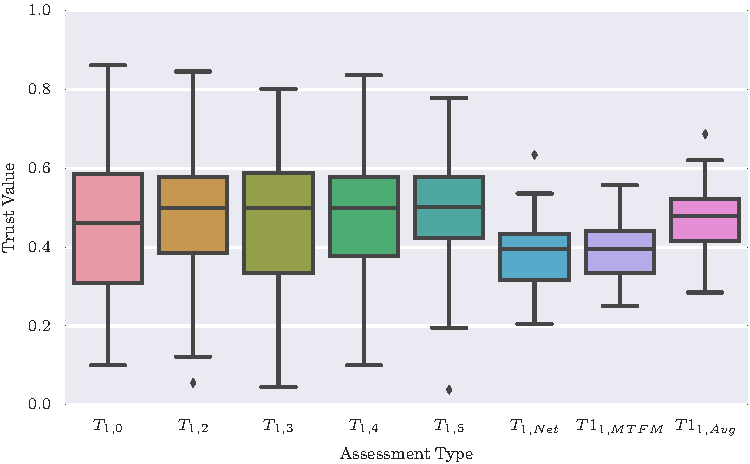
\includegraphics[width=.95\linewidth]{trust_bella_allbut1_mobile_selfish}
  \missingfigure[figwidth=.95\linewidth]{trust bella allbut1 mobile selfish}
  \caption{All Nodes but $n_1$ Randomly Walking}
  \label{fig:selfish_trust_allbut1}
\end{subfigure}
\begin{subfigure}{.5\textwidth}
\centering
  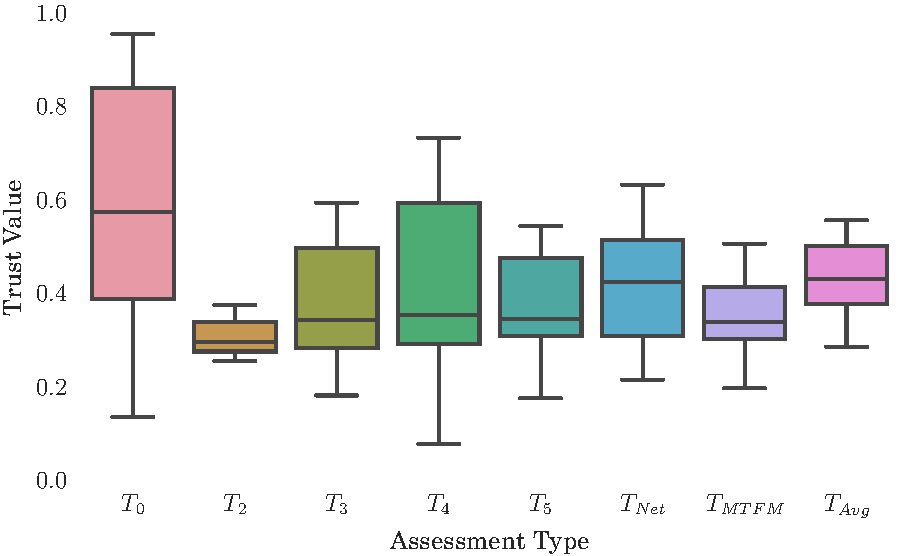
\includegraphics[width=.95\linewidth]{trust_bella_all_mobile_selfish}
  \caption{All Nodes Randomly Walking}
  \label{fig:selfish_trust_all_mobile}
\end{subfigure}
\caption{MTFM Trust assessments for varying mobility options in the selfish case}
\label{fig:trust_mobility}
\end{figure}



\begin{figure}
\begin{subfigure}{0.5\textwidth}
  \centering
  %\includegraphics[width=.95\linewidth]{beta_trust_bella_static_joint}
  \missingfigure[figwidth=.95\linewidth]{beta trust bella static joint}
  \caption{All Nodes Static}
  \label{fig:beta_trust_static}
\end{subfigure}%
\begin{subfigure}{0.5\textwidth}
  \centering
  %\includegraphics[width=.95\linewidth]{beta_trust_bella_single_mobile_joint}
  \missingfigure[figwidth=.95\linewidth]{beta trust bella single mobile joint}
  \caption{$n_1$ Randomly Walking}
  \label{fig:beta_trust_single}
\end{subfigure}%

\begin{subfigure}{0.5\textwidth}
\centering
  %\includegraphics[width=.95\linewidth]{beta_trust_bella_allbut1_mobile_joint}
  \missingfigure[figwidth=.95\linewidth]{beta trust bella allbut1 mobile joint}
  \caption{All Nodes but $n_1$ Randomly Walking}
  \label{fig:beta_trust_allbut1}
\end{subfigure}%
\begin{subfigure}{0.5\textwidth}
\centering
  %\includegraphics[width=.95\linewidth]{beta_trust_bella_all_mobile_joint}
  \missingfigure[figwidth=.95\linewidth]{beta trust bella all mobile joint}
  \caption{All Nodes Randomly Walking}
  \label{fig:beta_trust_all_mobile}
\end{subfigure}
\caption{Beta Trust time varying assessments for of $n1$ varying mobility options}
\label{fig:trust_mobility}
\end{figure}



\section{UNEDITED PROSE: Real Time Grey Systems}
\emph{Incoming Train of Consciousness}


For a given metric set $X$ such that $X = {x_1,\dots,x_M}$ representing the $M$ different types of measurement generated by an observer. If these metrics are not synchronised, for instance if they are interrupt driven such as communications-based observations, generating more abstract measurements requires inherent assumptions about ``how to accumulate the data while you wait''. For instance, in \cite{Bolster2015}, we demonstrated a periodic trust assessment framework for autonomous marine environments, in such an environment, to establish useful, generalised, data, it was necessary to wait for a relatively long time to accumulate enough data to make assessments.
However, this left many 'smells'; data was being left in-buffer for a long time before being used to make decisions, and by the time the data was collated and processed, it could be wildly different from the reality. Further, while some periods could be extremely sparse or even empty, others could be extremely busy with many records having to be averaged down to provide a 'single period' response. 
Therefore, the implementation of a suitable sequence buffer version of the framework would be beneficial.

Such a sequence buffer framework would involve a tracking predictor that would provide best-guess estimates of an interpolated value for a metric between value updates, and a back-propagation algorithm to retroactively update historical assessments of that metrics so as to better inform any abstracted trust value predictor.

I had initially thought that such a back-propagator would be a total mess as I'd imagined that significant-model-breaking would potentially indicate untrustworthy behaviour, but this is stupid since the per-metric-model has the least information of anyone and is simply there to provide better intermediate values and has no / limited direct impact on the overall trust behaviour. 

This back propagation will probably be a pain to implement as it'd require a retroactive reassessment of trust and could get really messy if it was interrupt driven, but it's better not to prematurely optimise.


\section{From end of Defense Trust Conclusions}
In order to contextualise the discussions on trust in mixed and hybrid networks, an exemplar scenario is considered.
That scenario builds on existing Maritime Autonomy Framework (MAF) investigations(Mollet, J. et al., 2012. Osprey Task 37 Activity 8 - Unmanned Systems Operations: Technical Assurance Work Package - Security Issues and Mitigations - Final Report,)

While the initial assessment does not cover the MHPC PT CONUSE recommendations, it provides a starting point for future trust research in UxV operations.
In order to constrain the scope of this project, a single operational scenario will be analysed within documented MCHP CONUSE(Rudge, A., Chapman, K. \& Goddard, N., 2012. Information Management for MHPC: Research Strategy,), of Route/Area Survey within both peacetime and wartime contexts, with a Beyond Line of Sight (BLOS) operator.
This scenario will be a minimal MCM operation in a littoral area.
In field assets will consist of:
\begin{itemize}
  \item Two squads consisting of Three UUV’s, (tacitly modelled on the in-service REMUS 100 UUV), and a USV providing acoustic-RF relay capabilities per-squad
  \item	an UAV providing BLOS Comms
  \item	A remote human operator (MCMV / PJHQ / etc)
\end{itemize}

\missingfigure{Indicitive Future MCM Scenario}

The differential between the peacetime and wartime contexts will be an attempted capture of a UUV by a manned surface-based FIS asset.
Clearly, this paper has a limited scope and does not attempt to cover every aspect of a trustworthy system.


	% Appendix Title

% Appendix B - Human Factors

\chapter{Human Factors related to Trusted Operation of Autonomous Systems}
\label{AppendixB}
\lhead{Appendix B. \emph{Human Factors related to Operational Trust}}

This work has largely considered autonomous systems as entities of wider systems, implicitly involving human operators/agents in some part of the desired operation.
We refer to these systems as \gls{acs}.
As described in~\autoref{Chapter3}, Operational Trust has two main aspects, trust in the system to behave as expected and trust in the interfaces between systems (human/machine and machine/machine).
Of all of the interfaces in an Autonomous Collaborative System, the most problematic is that arguably that between the \gls{acs} and the human operator / team of operators.
Cummings identified the main challenges to \gls{hsc}, summarised below:\cite{Cummings2010}

\subsubsection{Information Overload}
Operator efficiency exhibits an optimum at moderate levels of cognitive engagement, above which cognitive ability is overloaded and performance drops (Otherwise known as the Yerkes-Dodson Law).
Additionally, in the case of under-engagement, operators can fall foul of boredom, and become desensitised to changing factors.
\textit{However, predicting this point of over-saturation is an open psychophysiological research problem.}

\subsubsection{Adaptive Automation}
Automation is well tailored to consistent levels of activity.
This is quite simply not the case many domains.
Particularly in defence and military applications, activity is characterised by long periods of ``routine'' punctuated by high intensity, usually unpredictable, activity.
At those interfaces between ``calm'' and ``storm'', where real time situational awareness is imperative, temporary Information Overload is highly probable.
Adaptive Automation enables autonomous systems to increase their \gls{loa} based on specific events in the task environment, changes in operator performance or task loading, or physiological methods.
It is taken as given that for routine operations, and increased \gls{loa} reduces operator workload, and vice versa.
However, this relationship is highly task dependent and can create severe problems in cases of \gls{loa} being greater, or indeed lesser, than is required.
In the cases of overly-high \gls{loa}, operator skill is degraded, situational awareness is reduced as the operator is not as engaged, and the automated system may not be able to handle unexpected events, requiring the operator to take over, which, given the previous points, is a difficult prospect.
Alternatively, in sub-optimal \gls{loa}, Information Overload can result in the case of high intensity situations, but also the system can fall foul of overly-sensitive human cognitive biases, false positive pattern detection, boredom, and complacency in the case where less is going on.
Therefore, as a corollary to Information Overload challenges, there is a need to define the interrelationship between levels of situational activity (or risk) and appropriate levels of automation.
\textit{Under what circumstances can AA be used to change the \gls{loa} of a system?
Does the autonomous system or the human decide to change \gls{loa}\@? 
What \gls{loa}s are appropriate for what circumstances?}

\subsubsection{Distributed Decision Making}
In a modern, non-hierarchical, often distributed or cellular military management system (Network Centric Warfare doctrine for example), tools are increasingly being used to mitigate information asymmetry within command and control.
A simple example of this is shared watch-logs in Naval operations, providing temporal collaboration between watch-teams separated in time.
The DoD Global Information Grid is another example of a spatial collaborative framework.
Recent work has demonstrated the power of collaborative analysis and human-machine shared sensing technologies even with low levels of training on the part of the operators providing superior results and resource efficiencies than either humans or machines alone in survey and search-and-rescue scenarios (Ahmed et al.2014)\todo{Check Security}.
As these temporal and spatial collaboration tools increase in complexity and ability, decisions that previously required SA that was only available at higher echelons within the standard hierarchy are available to commanders on the ground, or even to individual team members, enabling the potential for informed decisions to be taken faster and more effectively, enabled by automated strategies to present relevant information to teams based on the operational context.
However there are a range of operational, legal, psychological and technical challenges that need to be addressed before confidence in these distributed management structures can be established.
Studies into situational awareness sharing techniques (telepresent table-top environments, video conferencing, and interactive whiteboards) have generally yielded positive results, however investigations into interruptive-communications (such as instant messaging chat) have demonstrated a negative impact on operational efficiency.
In short, the biggest problem with distributed decision making in the context of supervisory systems is that \textit{there is no consensus on whether it is advantageous or not, and what magnitude of operational delta is introduced, if any.}

\subsubsection{Complexity}
Beyond simple Information Overload, increasing complexity of information presented to operators is having a negative effect on operational efficiency.
In HSC, displays are designed to reduce complexity, introducing abstractions with an aim to presenting the minimum amount of information to the operator required to maintain an accurate and up-to-date mental model of the environmental and operational state.
This has led to the development of many domain specific decision support interfaces, however, in academic research, there has been nothing but ‘mixed results’.
One commonly raised negative is the general bias on the ‘cool factor’ of interfaces.
Immersive 3D visual, aural, or haptic interfaces that at first appraisal seem to provide more approachable information to the operator, and are indeed tacitly preferred by operators in use.
However, there has not been any evidence to demonstrate performance improvement when using these tools, and in-fact, \textit{improving the ``fidelity'' of the interfaces has led to operators’ overly-relying on these representations of the environment rather than remaining engaged in the environment.}

\subsubsection{Cognitive Biases and Failing Heuristics}
In many areas, operators and commanders are required to make rapid decisions with imperfect information, driven by massively increased information availability and rates of change in areas such as battlefield tactics and global finance markets.
However, Human decision making isn’t always rational (especially under pressure), and operators use personally derived heuristics to make ``rational shortcuts''.
This is a double edged sword, where these heuristics can be employed to greatly reduce the normative cognitive load in a stressful situation, but also introduce destructive biases, where these shortcuts make assumptions that don’t bear out in reality.

For example, in the context of decision support systems, ``Autonomy Bias'' has been observed as a complement to the already well known ``Confirmation Bias''\footnote{Confirmation Bias is the tendency for people to preferentially select from available information that information that supports pre-existing beliefs or hypotheses.}  and ``Assimilation Bias''\footnote{Assimilation Bias is often thought of as a subset of Confirmation Bias, whereby it specifies that instead of seeking out information supporting of current views, any incoming data is interpreted as being supportive of a particular view without questioning that view, even if it appears contradictory.}, where operators that have been provided with a ``correct'' answer by a decision support system do not look (or see, depending on perspective) for any contradictory information, and will unquestionably follow, increasing error rates significantly.

This behaviour isn't only the reserve of decision support systems, but also in the generic allocation of operator attention; scheduling heuristics are used to decide how much time tasks should be worked on, and time and again, humans are found to be far from optimal in this regard, especially in time-pressured scenarios where these heuristics are in even more demand.
Even when operators are given optimal scheduling rules, these quickly fall apart, often due to primary task efficiency degradation after interruption.
This highlights a critical interface in the adoption of complex autonomous systems that still demand ‘Man in the loop’ functionality; if a system is required to have full-time concentrated supervision (e.g.\ flying a UCAV), but also event-based reactive decision making (e.g.\ alerts from non-critical subsystems), both tasks are negatively impacted.
In an assessment of factors influencing trust in autonomous vehicles and medical diagnosis support systems, Carlson et al also identified that a major factor in an operator or users’ trust in a system was not only dependant on past performance and current accuracy but also on ``soft factors'' such as the branding and reputation of the manufacture / designer. (Carlson et al. 2014)\todo{Check Security}
Further, autonomous decision support / detection / classification systems have an ``uncanny valley'' to overcome in terms of accuracy, in that there is a dangerous period when such systems are used but not perfect, but operators become complacent, causing an increased error rate, until such a time that those autonomous systems can match or exceed the detection rates of their human counterparts. % Appendix Title

% Appendix C - Grey Theory

\chapter{Grey System Theory and Grey Trust Assessmen}
\label{apx:grey}
\lhead{Appendix C. \emph{Grey System Theory and Grey Trust Assessment}}

\section{Grey numbers, operators and terminology}
Grey numbers are used to represent values where their discrete value is unknown, where that number may take its possible value within an interval of potential values, generally written using the symbol $\oplus$.
Taking $a$ and $b$ as the lower and upper bounds of the grey interval respectively, such that $\oplus \in [a,b] | a < b$ 
The ``field'' of $\oplus$ is the value space $[a,b]$.
There are several classifications of grey numbers based on the relationships between these bounds.\todo{don't think classification is the right word here}
Black and White numbers are the extremes of this classification; such that $\dot\oplus \in [-\infty, +\infty]$ and $\mathring\oplus \in [x, x] | x \in \mathbb{R}$ or $\oplus(x)$
It is clear that white numbers such as $\mathring\oplus$ have a field of zero while black numbers have an infinite field.

Grey numbers may represent partial knowledge about a system or metric, and as such can represent half-open concepts, by only defining a single bound; for example $\underline\oplus = \oplus(\underline x ) \in [x, +\infty]$ and $\overline\oplus = \oplus(\overline x) \in [-\infty, x]$.

Primary operations within this number system are as follows;
\begin{subequations}
  \begin{align}
    \oplus_1 + \oplus_2      &\in [a_1+a_2,b_1+b_2] \label{eq:grey_add}\\
    -\oplus         &\in [-b,-a] \label{eq:grey_neg} \\
    \oplus_1 - \oplus_2      &= \oplus_1+(-\oplus) \label{eq:grey_sub}\\
    \oplus_1 \times \oplus_2 &\in \begin{aligned}[t]
      &[\min(a_1 a_2, a_1 b_2, b_1 a_2, b_2 a_2), \\
      & \max(a_1 a_2, a_1 b_2, b_1 a_2, b_2 a_2)]
    \end{aligned} \label{eq:grey_mult}\\
    \oplus^{-1} &\in [b^{-1}, a^{-1}] \label{eq:grey_inv}\\
    \oplus_1 / \oplus_2 & = \oplus_1 \times \oplus_2^{-1} \label{eq:grey_div} \\
    \oplus \times k &\in [ka,kb] \label{eq:grey_times_scalar}\\
    \oplus^k &\in [a^k, b^k] \label{eq:grey_exp}
  \end{align}
\end{subequations}
where $k$ is a scalar quantity.

\section{Whitenisation and the Grey Core}
The characterisation of grey numbers is based on the encapsulation of information in a grey system in terms of the grey numbers core ($\hat\oplus$) and it's degree of greyness ($g^\circ$).
If the distribution of a grey number field is unknown and continuous, $\hat\oplus = \frac{a + b}{2}$.

Non-essential grey numbers are those that can be represented by a white number obtained either through experience or particular method. \cite{Liu2011}
This white value is represented by $\tilde\oplus$ or $\oplus(x)$ to represent grey numbers with $x$ as their whitenisation.
In some cases depending on the context of application, particular gray numbers may temporarily have no reasonable whitenisation value (for instance, a black number).
Such numbers are said to be Essential grey numbers.

\section{Grey Sequence Buffers and Generators}
\todo{eqs of sequence buffers and partial derivs}
Given a fully populated value space, sequence buffer operations are used to provide abstractions over the dataspace.
These abstractions can be \emph{weakening} or \emph{strengthening}.
In the weakening case, these operations perform a level of smoothing on the volatility of a given input space, and strengthening buffers serve to highlight and 
A powerful tool in grey system theory is the use of grey incidence factors, comparing the ``likeness'' of one value against a cohort of values.
This usefulness applies particularly well in the case of multi-agent trust networks, where the aim is to detect and identify malicious or maladaptive behaviour, rather than an absolute assessment of ``trustworthiness''.

\section{Grey Trust}
Grey Theory performs cohort based normalization of metrics at runtime.
This creates a more stable contextual assessment of trust, providing a ``grade'' of trust compared to other observed entities in that interval, while maintaining the ability to reduce trust values to a stable assessment range for decision support without requiring every environment entered into to be characterised.
Grey assessments are relative in both fairly and unfairly operating cohorts.
Entities will receive mid-range trust assessments if there are no malicious actors as there is no-one else ``bad'' to compare against.

Guo\cite{Guo11} demonstrated the ability of Grey Relational Analysis (GRA)\cite{Zuo1995} to normalise and combine disparate traits of a communications link such as instantaneous throughput, received signal strength, etc.\ into a Grey Relational Coefficient, or a ``trust vector''.

In \cite{Guo11}, the observed metric set $X = {x_1,\dots,x_M}$ representing the measurements taken by each node of its neighbours at least interval, is defined as $X=[$packet loss rate, signal strength, data rate, delay, throughput$]$.
The trust vector is given as
%
\begin{align}
  \label{eq:grc}
  \theta_{k,j}^t = \frac{\min_k|a_{k,j}^t - g_j^t| + \rho \max_k|a_{k,j}^t-g_j^t|}{|a_{k,j}^t-g_j^t| + \rho \max_k|a_{k,j}^t-g_j^t|} \\
  \phi_{k,j}^t = \frac{\min_k|a_{k,j}^t - b_j^t| + \rho \max_k|a_{k,j}^t-b_j^t|}{|a_{k,j}^t-b_j^t| + \rho \max_k|a_{k,j}^t-b_j^t|} \notag 
\end{align}
%
where $a_{k,j}^t$ is the value of a observed metric $x_j$ for a given node $k$ at time $t$, $\rho$ is a distinguishing coefficient set to $0.5$, $g$ and $b$ are respectively the '``good'' and ``bad'' reference metric sequences from $\{a_{k,j}^t k=1,2\dots K\}$, e.g.\ $g_j=\max_k({a_{k,j}^t})$,  $b_j=\min_k({a_{k,j}^t})$ (where each metric is selected to be monotonically positive for trust assessment, e.g.\ higher throughput is always better).

Weighting can be applied before generating a scalar value which allows the identification and classification of untrustworthy behaviours.

%
\begin{equation}
  \label{eq:metric_weighting}
  [\theta_k^t, \phi_k^t] = \left[\sum_{j=0}^M h_j \theta_{k,j}^t,\sum_{j=0}^M h_j \phi_{k,j}^t \right]
\end{equation}
Where $H=[h_0\dots h_M]$ is a metric weighting vector such that $\sum h_j = 1$, and in the basic case, $H=[\frac{1}{M},\frac{1}{M}\dots\frac{1}{M}]$ to treat all metrics evenly.
$\theta$ and $\phi$ are then scaled to $[0,1]$ using the mapping $y = 1.5 x - 0.5$.
The $[\theta,\phi]$ values are reduced into a scalar trust value by $T_k^t = ({1+{(\phi_k^t)^2}/{(\theta_k^t)^2}})^{-1}$.
This trust value minimises the uncertainties of belonging to either best ($g$) or worst ($b$) sequences in \eqref{eq:grc}.

\acrshort{mtfm} combines this GRA with a topology-aware weighting scheme\eqref{eq:networkeffects} and a fuzzy whitenization model\eqref{eq:whitenization}.
There are three classes of topological trust relationship used; Direct, Recommendation, and Indirect.
Where an observing node, $n_i$, assesses the trust of another, target, node, $n_j$; the Direct relationship is $n_i$'s own observations $n_j$'s behaviour.
In the Recommendation case, a node $n_k$, which shares Direct relationships with both $n_i$ and $n_j$, gives its assessment of $n_j$ to $n_i$.
The Indirect case, similar to the Recommendation case, the recommender $n_k$, does not have a direct link with the observer $n_i$ but $n_k$ has a Direct link with the target node, $n_j$.
These relationships give us node sets, $N_R$ and $N_I$ containing the nodes that have recommendation or indirect, relationships to the observing node respectively.
%
\begin{align}
  \label{eq:networkeffects}
  T_{i,j}^{\acrshort{mtfm}}=\frac{1}{2} \cdot \max_s\{f_s(T_{i,j})\} T_{i,j}+&\frac{1}{2} \frac{2|N_R| }{2|N_R| + |N_I|}\sum_{n \in N_R} \max_s\{f_s(T_{i,n})\} T_{i,n}\\ \notag
  +&\frac{1}{2} \frac{|N_I| }{2|N_R| + |N_I|}\sum_{n \in N_I} \max_s\{f_s(T_{i,n})\} T_{i,n} 
\end{align}
Where $T_{i,n}$ is the subjective trust assessment of $n_i$ by $n_n$, and $f_s = [ f_1,f_2, f_3]$ given as:
\begin{align}
  \label{eq:whitenization}
  f_1(x)&= -x+1\notag\\
  f_2(x)&= 
  \begin{cases}
    2x & \text{if }x\leq 0.5\\
    -2x+2 & \text{if }x>0.5
  \end{cases}\\
  f_3(x)&= x\notag
\end{align}

Grey System Theory, by it's own authors admission, hasn't taken root in it's originally intended area of system modelling \cite{Liu2011}.
However, given it's tentative application to \gls{manet} trust, taking a Grey approach on a per metric benefit has qualitative benefits that require investigation; the algebraic approach to uncertainty and the application of ``essential and non essential greyness'', whiteisation, and particularly grey buffer sequencing allow for the opportunity to generate continuous trust assessments from multiple domains asynchronously.

 % Appendix Title

\addtocontents{toc}{\vspace{2em}}  % Add a gap in the Contents, for aesthetics
\backmatter

%% ----------------------------------------------------------------
\label{Bibliography}
\lhead{\emph{Bibliography}}  % Change the left side page header to "Bibliography"
\bibliographystyle{unsrtnat}
% \bibliographystyle{unsrtnat}  % Use the "unsrtnat" BibTeX style for formatting the Bibliography
\bibliography{Thesis}  % The references (bibliography) information are stored in the file named "Thesis.bib"

\end{document}  % The End
%% ----------------------------------------------------------------
